%\documentclass[11pt]{book}
%
%\setlength{\parindent}{0pt}
%\setlength{\parskip}{8pt}
%
%\usepackage{amsmath}
%\usepackage{amssymb}
%\usepackage{hyperref}
%
%\renewcommand*{\thefootnote}{\fnsymbol{footnote}}
%
%\setcounter{chapter}{2}
%
%\begin{document}
%
%\section*{A Levelized Comparison of \\ Pulsed and Steady-State Tokamaks}
%
%\let\cleardoublepage\relax \tableofcontents \newpage

\chapter{Formalizing the Systems Model}

\label{chapter:model}

The goal of this chapter is to take a step back from the steady current derivation and see the larger picture behind reactor design. As such, a more in-depth description of \replaced{static}{fixed} and \replaced{dynamic}{floating} variables is given. This discussion of \replaced{dynamic}{floating} variables will then lend itself to a description of the framework underpinning the fusion systems model. As such, we will now need formulas for the radius and magnet strength of the tokamak. Moving forward, the current will \deleted{then} remain a connecting piece as we \replaced{redirect focus}{switch gears} to pulsed tokamaks and compare \replaced{the underlying solvers of the two schemes.}{the two schemes' underlying solvers.}

\added{The end result of this analysis will then be equations that allow the density ($\overline n$), current ($I_P$), major radius ($R_0$), and magnet strength ($B_0$) to be written as functions of the temperature ($\overline T$) and  static variables (e.g.\ $\nu_n$, $N_G$, $f_D$). These formulas are the product of applying constraints required for all tokamak reactors with several other limiting constraints. The constraints relevant to all tokamak reactors are: the Greenwald limit, current balance, and power balance. Limit constraints then include: the Troyon beta limit, the kink safety factor, the wall loading limit, the maximum power constraint, and the heat loading limit.}

\added{Actual methodologies for solving for the five dynamic variables simultaneously -- i.e.\ $\overline T$, $\overline n$, $I_P$, $R_0$, $B_0$ -- are put off until \cref{chapter:complete}.}

\section{Explaining \replaced{Static}{Fixed} Variables} 

In this model, \replaced{static}{fixed} variables are ones that remain constant while solving for a reactor. These include geometric scalings (i.e.\ $\epsilon$, $\delta$, $\kappa$), profile parameters (i.e.\ $\nu_n$, $\nu_T$, $l_i$), and a \replaced{couple dozen}{slew} of physics constants related to pulsed and steady-state design (e.g.\ Q, $N_G$, $f_D$). For a complete list of \replaced{static}{fixed} variables, consult \replaced{\cref{chapter:var_table}}{the appendix}. The point to make now is that this model treats \replaced{static}{fixed} variables as \replaced{immutable}{second-class} objects. As such they often reside in \replaced{static}{fixed} coefficients -- $K_\square$ -- which are treated as constants.

\section{Connecting \replaced{Dynamic}{Floating} Variables}

\replaced{Dynamic}{Floating} variables -- $\overline T$, $\overline n$, $I_P$, $R_0$, $B_0$ -- are the first-class variables of this fusion systems model. They represent the fundamental properties of a plasma and tokamak (which constitute a fusion reactor). As such, they will be reintroduced one at a time, explaining how they fit into the model -- and which \replaced{equations are}{equation is} capable of representing \replaced{them}{it}.

\begin{table}[h!]
\centering	
\caption{Dynamic Variables}
\begin{tabular}{ c|c|c } 

\textbf{Symbol} & \textbf{Name} & \textbf{Units} \\
\hline
$I_P$ & Plasma Current & MA \\ 
$\overline{T}$ & Plasma Temperature & keV \\ 
$\overline{n}$ & Electron Density & $10^{20} \, \textnormal{m}^{-3}$ \\ 
$R_0$ &  Major Radius & m \\ 
$B_0$ &  Magnetic Field & T
\end{tabular}
\label{table:dynamic}
\end{table}

Bluntly, this fusion systems model is a simple algebra problem: solve five equations with five unknowns (i.e.\ $\overline T$, $\overline n$, $I_P$, $R_0$, $B_0$). Although this naive approach would work, we can do a little better by \replaced{collapsing}{wrangling} these five equations down to just one. This was already done while deriving the steady current. It just happened that the current was not directly dependent on the tokamak size ($R_0$) or magnet strength ($B_0$). 

This will prove more challenging for the generalized current needed for pulsed operation. Even so, this equation will still be \replaced{reduced}{boiled down} to one equation with a single unknown -- $I_P$. A solution to which can be solved much faster than the naive 5 equation approach. This is one reason the model is so fast. 

\subsubsection{The Plasma Temperature -- $\overline T$}

The plasma temperature, measured in keV (kilo-electron-volts), is one of the most \replaced{nonlinear}{finicky} variables in the fusion systems \replaced{framework}{model}. It first proved troublesome when it was shown that a pedestal profile -- not a parabolic one used here -- would be needed for an accurate calculation of bootstrap current. The \replaced{black-box}{unusual} tabulation for reactivity -- ($\sigma v$) -- which appeared in fusion power only further exposed this nonlinearity.

Acknowledging that temperature is the most difficult to handle parameter prompts its use as the scanned variable. What this means practically is scanning temperatures \replaced{is the most straightforward method to produce}{produces} curves of reactors. By example, a scan may be run over the average temperatures ($\overline T$): 10, 15, 20, 25, and 30 keV -- \added{where} each \replaced{corresponds}{corresponding} to its own reactor \added{with its own field strength ($B_0$), plasma current ($I_P$), etc}. In equation form, this becomes:
\begin{equation}
	\label{eq:tbar}
	\overline T = const.
\end{equation}
\myequations{Scanned Temperature -- $\overline T$}
\replaced{The constant value, here,}{Where the constant} happens to be 10 \added{keV} in one run, 15 \added{keV} for the next, and 30 \added{keV} in the fifth.

\subsubsection{The Plasma Density -- $\overline n$}

\replaced{The Greenwald density limit is a constraint with a simple form that applies to all tokamak reactors.}{The cornerstone of this fusion systems model has always been the application of the Greenwald density limit from square one.} It is for this reason -- as well as being a good approximation -- that a parabolic profile was rationalized over a pedestal (H-Mode) one. Repeated, the Greenwald density limit is:
\begin{equation}
	\tag{\ref{eq:greenwald}}
	\overline n = K_n \cdot \frac{I_P}{R_0^2}
\end{equation}
This is an exceptionally simple relationship and why it guided the model. Unlike the next three variables, it is actually used in their derivations. \deleted{Therefore, any reactor found through this model is considered a \emph{Greenwaldian Reactor} -- one held at the Greenwald density limit.}

\subsubsection{The Plasma Current -- $I_P$}

The plasma current is what separates steady-state from pulsed operation. From before, the steady current was found to be:
\begin{equation}
	\tag{\ref{eq:steady}}
	I_P = \frac{K_{BS} \overline T}{1 - K_{CD} ( \sigma v ) }
\end{equation}
This was derived by setting the total current equal to the two sources of current: bootstrap and current drive. Or in fractional form,
\begin{equation}
	I_P = I_{BS} + I_{CD} \ \ \rightarrow \, \ \ 1 = f_{BS} + f_{CD}
\end{equation}
This says that the current fractions of bootstrap and current drive must sum to one. As shown next chapter, inductive sources can be included into this current balance:
\begin{equation}
	\label{eq:ifbal}
	1 = f_{BS} + f_{CD} + f_{ID}
\end{equation}
\begin{figure}
	\centering
	\begin{adjustbox}{width=0.75\textwidth}
		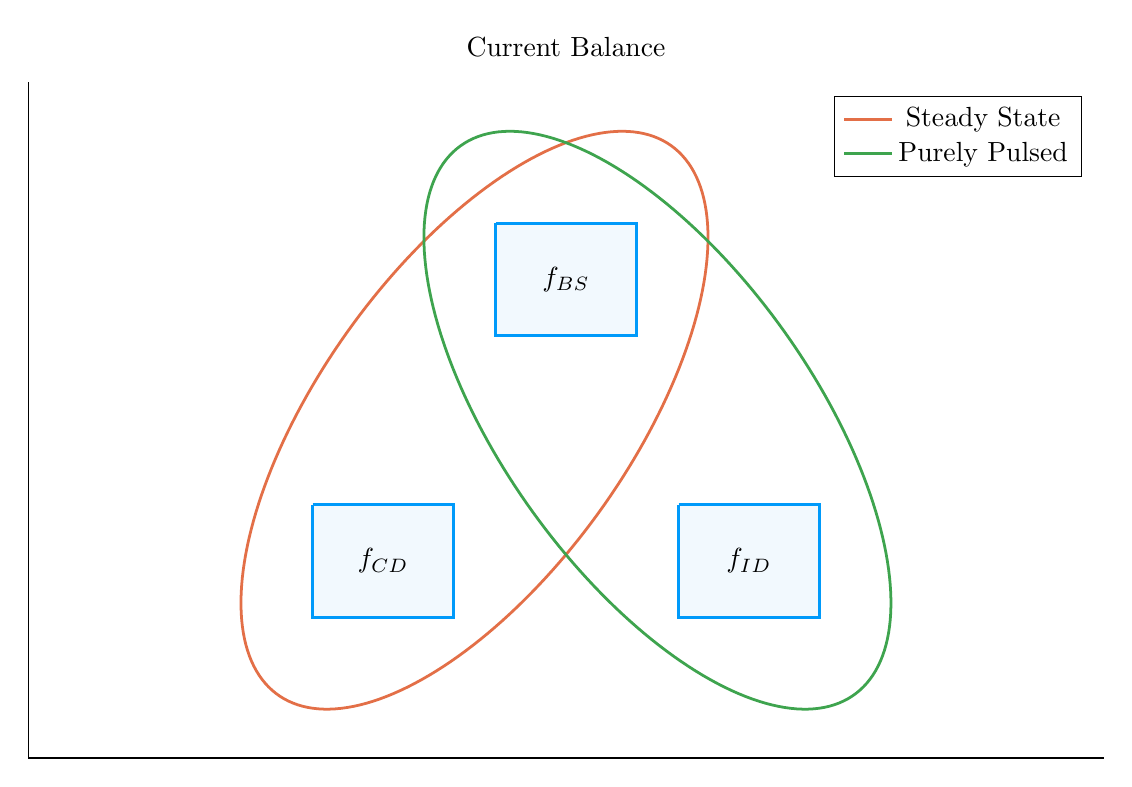
\begin{tikzpicture}[]
\begin{axis}[height = {101.6mm}, axis equal = {true}, ylabel = {}, title = {Current Balance}, xmin = {-5.773116112756781}, xmax = {5.773116112756781}, ymax = {6}, xlabel = {}, {unbounded coords=jump, scaled x ticks = false, xticklabel style={rotate = 0}, xmajorticks=false, xmajorgrids = false, axis lines* = left, scaled y ticks = false, yticklabel style={rotate = 0}, ymajorticks=false, ymajorgrids = false, axis lines* = left,     xshift = 0.0mm,
    yshift = 0.0mm,
    axis background/.style={fill={rgb,1:red,1.00000000;green,1.00000000;blue,1.00000000}}
}, ymin = {-6}, width = {152.4mm}]\addplot+ [color = {rgb,1:red,0.00000000;green,0.60560316;blue,0.97868012},
draw opacity=1.0,
line width=1,
solid,mark = none,
mark size = 2.0,
mark options = {
    color = {rgb,1:red,0.00000000;green,0.00000000;blue,0.00000000}, draw opacity = 1.0,
    fill = {rgb,1:red,0.00000000;green,0.60560316;blue,0.97868012}, fill opacity = 1.0,
    line width = 1,
    rotate = 0,
    solid
},fill = {rgb,1:red,0.00000000;green,0.60560316;blue,0.97868012}, fill opacity=0.05,forget plot]coordinates {
(-1.25, 3.5)
(1.25, 3.5)
(1.25, 1.5)
(-1.25, 1.5)
(-1.25, 3.5)
};
\addplot+ [color = {rgb,1:red,0.00000000;green,0.60560316;blue,0.97868012},
draw opacity=1.0,
line width=1,
solid,mark = none,
mark size = 2.0,
mark options = {
    color = {rgb,1:red,0.00000000;green,0.00000000;blue,0.00000000}, draw opacity = 1.0,
    fill = {rgb,1:red,0.00000000;green,0.60560316;blue,0.97868012}, fill opacity = 1.0,
    line width = 1,
    rotate = 0,
    solid
},fill = {rgb,1:red,0.00000000;green,0.60560316;blue,0.97868012}, fill opacity=0.05,forget plot]coordinates {
(-4.5, -1.5)
(-2.0, -1.5)
(-2.0, -3.5)
(-4.5, -3.5)
(-4.5, -1.5)
};
\addplot+ [color = {rgb,1:red,0.00000000;green,0.60560316;blue,0.97868012},
draw opacity=1.0,
line width=1,
solid,mark = none,
mark size = 2.0,
mark options = {
    color = {rgb,1:red,0.00000000;green,0.00000000;blue,0.00000000}, draw opacity = 1.0,
    fill = {rgb,1:red,0.00000000;green,0.60560316;blue,0.97868012}, fill opacity = 1.0,
    line width = 1,
    rotate = 0,
    solid
},fill = {rgb,1:red,0.00000000;green,0.60560316;blue,0.97868012}, fill opacity=0.05,forget plot]coordinates {
(2.0, -1.5)
(4.5, -1.5)
(4.5, -3.5)
(2.0, -3.5)
(2.0, -1.5)
};
\addplot+ [color = {rgb,1:red,0.88887350;green,0.43564919;blue,0.27812294},
draw opacity=1.0,
line width=1,
solid,mark = none,
mark size = 2.0,
mark options = {
    color = {rgb,1:red,0.00000000;green,0.00000000;blue,0.00000000}, draw opacity = 1.0,
    fill = {rgb,1:red,0.88887350;green,0.43564919;blue,0.27812294}, fill opacity = 1.0,
    line width = 1,
    rotate = 0,
    solid
}]coordinates {
(1.8698661812068136, 4.877080107549691)
(1.7975582266118808, 4.9252162522328415)
(1.7218385915440537, 4.9684428342438745)
(1.6427827549822935, 5.006716764385765)
(1.5604695215037632, 5.03999989037258)
(1.4749809427297138, 5.068259034860505)
(1.3864022355346433, 5.091466028519745)
(1.2948216971002622, 5.109597738114323)
(1.2003306168989445, 5.122636089561793)
(1.1030231856943935, 5.130568085949879)
(1.0029964016502424, 5.133385820492077)
(0.9003499736401737, 5.131086484409318)
(0.7951862218559462, 5.123672369729815)
(0.6876099758124048, 5.111150867004319)
(0.5777284698511354, 5.093534457939059)
(0.46565123624694493, 5.07084070295371)
(0.35148999602370634, 5.043092223676775)
(0.23535854758841435, 5.010316680395862)
(0.11737265329445545, 4.972546744485303)
(-0.00235007595282255, 4.929820065838624)
(-0.12369029793321751, 4.882179235338303)
(-0.2465270580745944, 4.829671742400261)
(-0.37073791002303214, 4.77234992763537)
(-0.49619903770001583, 4.710270930675205)
(-0.6227853787249911, 4.643496633214007)
(-0.7503707490802689, 4.572093597323671)
(-0.878827968893996, 4.496132999103221)
(-1.0080289892158198, 4.415690557728926)
(-1.137845019658864, 4.330846459975782)
(-1.26814665678079, 4.241685280285592)
(-1.3988040130759585, 4.148295896461316)
(-1.5296868464501256, 4.050771401071749)
(-1.6606646900485882, 3.949209008654826)
(-1.7916069823083864, 3.8437099588120507)
(-1.9223831971049103, 3.734379415290662)
(-2.0528629738631725, 3.6213263611541278)
(-2.1829162475040724, 3.5046634901454468)
(-2.3124133780960925, 3.3845070943515854)
(-2.4412252800831986, 3.26097694828099)
(-2.5692235509601344, 3.1341961894697543)
(-2.696280599266827, 3.004291195735447)
(-2.822269771774333, 2.8713914592009493)
(-2.947065479735527, 2.735629457213896)
(-3.0705433240746993, 2.597140520290374)
(-3.192580219391261, 2.4560626972145165)
(-3.3130545166539442, 2.3125366174284774)
(-3.4318461244632026, 2.166705350849943)
(-3.5488366287609345, 2.0187142652569277)
(-3.6639094108681878, 1.8687108813820061)
(-3.776949763733194, 1.7168447258604496)
(-3.8878450062738565, 1.5632671821788118)
(-3.9964845957006974, 1.4081313397725874)
(-4.1027602377083205, 1.2515918414233274)
(-4.206565994425528, 1.0938047291073505)
(-4.307798390016492, 0.9349272884497156)
(-4.4063565138277205, 0.7751178919384804)
(-4.502142120977991, 0.614535841055565)
(-4.595059730290983, 0.4533412074815748)
(-4.685016719472996, 0.29169467353285894)
(-4.771923417440856, 0.12975737198989234)
(-4.8556931937080146, -0.032309274523392384)
(-4.936242544739693, -0.1943437144491822)
(-5.013491177191022, -0.3561844283338884)
(-5.087362087945198, -0.5176700898342566)
(-5.157781640871865, -0.6786397265309694)
(-5.224679640229201, -0.8389328803894542)
(-5.287989400636577, -0.9983897677079463)
(-5.347647813547976, -1.1568514383933535)
(-5.403595410159981, -1.3141599344061687)
(-5.455776420691558, -1.4701584472164726)
(-5.504138829976595, -1.6246914741140965)
(-5.548634429313749, -1.7776049732170973)
(-5.589218864521925, -1.9287465170240605)
(-5.625851680153492, -2.0779654443571474)
(-5.658496359821148, -2.225113010544426)
(-5.687120362598258, -2.3700425356918093)
(-5.711695155456349, -2.5126095508967543)
(-5.732196241707455, -2.6526719422580065)
(-5.74860318542295, -2.7900900925378296)
(-5.760899631804527, -2.9247270203354994)
(-5.769073323487013, -3.0564485166333526)
(-5.773116112756781, -3.1851232785792454)
(-5.773023969673565, -3.3106230403720964)
(-5.768796986087595, -3.432822701120024)
(-5.760439375548035, -3.551600449543642)
(-5.747959469102832, -3.6668378854001826)
(-5.731369706994138, -3.778420137507439)
(-5.710686626257609, -3.8862359782498594)
(-5.685930844237935, -3.9901779344526522)
(-5.657127038037011, -4.090142394513381)
(-5.624303919915274, -4.186029711684261)
(-5.587494208670695, -4.2777443034022165)
(-5.546734597023965, -4.365194746567642)
(-5.502065715042401, -4.448293868676952)
(-5.453532089639006, -4.526958834718015)
(-5.4011821001870715, -4.601111229741906)
(-5.345067930294576, -4.67067713702862)
(-5.285245515786418, -4.735587211768881)
(-5.221774488946376, -4.795776750188546)
(-5.154718119074351, -4.851185754046737)
(-5.084143249418149, -4.901758990443393)
(-5.010120230542682, -4.947446046876624)
(-4.932722850202994, -4.98820138149499)
(-4.852028259791015, -5.023984368494613)
(-4.768116897429388, -5.054759338615853)
(-4.681072407788987, -5.080495614699213)
(-4.590981558710103, -5.101167542264987)
(-4.497934154710361, -5.116754515086211)
(-4.40202294746563, -5.127240995729401)
(-4.303343543353135, -5.132616531042591)
(-4.201994308148942, -5.132875762575277)
(-4.098076268974807, -5.1280184319198305)
(-3.9916930135921564, -5.118049380969083)
(-3.88295058714354, -5.102978547089826)
(-3.7719573864445346, -5.082820953217027)
(-3.658824051931438, -5.0575966928786364)
(-3.543663357372476, -5.02733091016593)
(-3.4265900974524626, -4.9920537746693245)
(-3.3077209733429527, -4.951800451404678)
(-3.1871744763719843, -4.906611065760036)
(-3.065070769909341, -4.8565306634977725)
(-2.941531569585093, -4.801609165851993)
(-2.816680021960811, -4.741901319765965)
(-2.690640581774395, -4.677466643319172)
(-2.5635388878808865, -4.608369366398399)
(-2.435501638012921, -4.5346783666719865)
(-2.306656462485676, -4.456467100931064)
(-2.1771317969721977, -4.373813531866238)
(-2.047056754475925, -4.286800050352669)
(-1.9165609966280504, -4.1955133933210735)
(-1.785774604437966, -4.100044557296444)
(-1.654827948625708, -4.00048870769076)
(-1.523851559665576, -3.896945083940012)
(-1.3929759976705065, -3.7895169005801836)
(-1.26233172224694, -3.678311244360763)
(-1.132048962449818, -3.5634389674983264)
(-1.0022575869674537, -3.4450145771766545)
(-0.8730869746655892, -3.323156121403477)
(-0.7446658856197179, -3.1979850713376368)
(-0.6171223327642645, -3.069626200204022)
(-0.49058345428648176, -2.938207458916877)
(-0.3651753868923626, -2.803859848535569)
(-0.24102314007082093, -2.666717289679875)
(-0.11825047148150092, -2.526916489034983)
(0.0030202364095237577, -2.384596803079324)
(0.12266809832327996, -2.2399000991709683)
(0.2405738466689491, -2.09297061413119)
(0.3566199504324037, -1.9439548104660527)
(0.4706907323336891, -1.7930012303693847)
(0.5826724841366269, -1.6402603476527216)
(0.6924535799956866, -1.4858844177497015)
(0.7999245877270309, -1.3300273259445707)
(0.9049783778929097, -1.1728444339759707)
(1.0075102305906167, -1.0144924251689658)
(1.1074179398395505, -0.8551291482497284)
(1.20460191546238, -0.6949134599984598)
(1.2989652823586764, -0.534005066897528)
(1.3904139770721349, -0.3725643659325606)
(1.478856841555075, -0.210752284705227)
(1.564205714036751, -0.04873012101713625)
(1.6463755169049392, 0.11334061791535466)
(1.725284341513138, 0.27529837645501054)
(1.8008535298288972, 0.4369817115859278)
(1.8730077528418523, 0.598229453843409)
(1.9416750856533156, 0.7588808679712085)
(2.0067870791725912, 0.9187758131459416)
(2.0682788283485025, 1.0777549026089095)
(2.126089036868173, 1.2356596625463219)
(2.1801600782585133, 1.3923326900594108)
(2.2304380533295443, 1.5476178100670777)
(2.2768728439022907, 1.7013602309846187)
(2.3194181627676604, 1.8534066990233193)
(2.358031599826549, 2.0036056509571933)
(2.392674664365143, 2.1518073652044736)
(2.423312823423304, 2.2978641110733555)
(2.4499155362177776, 2.4416302960231726)
(2.4724562845859026, 2.5829626107941834)
(2.490912599419497, 2.7217201722613846)
(2.505266083062553, 2.857764663869852)
(2.5155024276504205, 2.990960473511697)
(2.521611429372199, 3.12117482870718)
(2.5235869986421147, 3.2482779289551793)
(2.5214271661697554, 3.3721430751211794)
(2.515134084923101, 3.4926467957337035)
(2.5047140279823985, 3.609668970063368)
(2.4901773822870172, 3.7230929478618506)
(2.471538638281525, 3.8328056656413696)
(2.448816375471295, 3.9386977593788552)
(2.422033243902053, 4.040663673532358)
(2.391215941581816, 4.1386017662611385)
(2.356395187867742, 4.232414410744436)
(2.317605692844403, 4.322008092498024)
(2.274886122724018, 4.4072935025914814)
(2.2282790613031342, 4.488185626673267)
(2.1778309675141685, 4.564603829714885)
(2.123592129114139, 4.636471936389625)
(2.06561661255673, 4.70371830700579)
(2.0039622090976756, 4.766275908918702)
(1.9386903771871857, 4.824082383350291)
(1.869866181206814, 4.877080107549691)
};
\addlegendentry{Steady State}
\addplot+ [color = {rgb,1:red,0.24222430;green,0.64327509;blue,0.30444865},
draw opacity=1.0,
line width=1,
solid,mark = none,
mark size = 2.0,
mark options = {
    color = {rgb,1:red,0.00000000;green,0.00000000;blue,0.00000000}, draw opacity = 1.0,
    fill = {rgb,1:red,0.24222430;green,0.64327509;blue,0.30444865}, fill opacity = 1.0,
    line width = 1,
    rotate = 0,
    solid
}]coordinates {
(-1.8698661812068136, 4.877080107549691)
(-1.7975582266118808, 4.9252162522328415)
(-1.7218385915440537, 4.9684428342438745)
(-1.6427827549822935, 5.006716764385765)
(-1.5604695215037632, 5.03999989037258)
(-1.4749809427297138, 5.068259034860505)
(-1.3864022355346433, 5.091466028519745)
(-1.2948216971002622, 5.109597738114323)
(-1.2003306168989445, 5.122636089561793)
(-1.1030231856943935, 5.130568085949879)
(-1.0029964016502424, 5.133385820492077)
(-0.9003499736401737, 5.131086484409318)
(-0.7951862218559462, 5.123672369729815)
(-0.6876099758124048, 5.111150867004319)
(-0.5777284698511354, 5.093534457939059)
(-0.46565123624694493, 5.07084070295371)
(-0.35148999602370634, 5.043092223676775)
(-0.23535854758841435, 5.010316680395862)
(-0.11737265329445545, 4.972546744485303)
(0.00235007595282255, 4.929820065838624)
(0.12369029793321751, 4.882179235338303)
(0.2465270580745944, 4.829671742400261)
(0.37073791002303214, 4.77234992763537)
(0.49619903770001583, 4.710270930675205)
(0.6227853787249911, 4.643496633214007)
(0.7503707490802689, 4.572093597323671)
(0.878827968893996, 4.496132999103221)
(1.0080289892158198, 4.415690557728926)
(1.137845019658864, 4.330846459975782)
(1.26814665678079, 4.241685280285592)
(1.3988040130759585, 4.148295896461316)
(1.5296868464501256, 4.050771401071749)
(1.6606646900485882, 3.949209008654826)
(1.7916069823083864, 3.8437099588120507)
(1.9223831971049103, 3.734379415290662)
(2.0528629738631725, 3.6213263611541278)
(2.1829162475040724, 3.5046634901454468)
(2.3124133780960925, 3.3845070943515854)
(2.4412252800831986, 3.26097694828099)
(2.5692235509601344, 3.1341961894697543)
(2.696280599266827, 3.004291195735447)
(2.822269771774333, 2.8713914592009493)
(2.947065479735527, 2.735629457213896)
(3.0705433240746993, 2.597140520290374)
(3.192580219391261, 2.4560626972145165)
(3.3130545166539442, 2.3125366174284774)
(3.4318461244632026, 2.166705350849943)
(3.5488366287609345, 2.0187142652569277)
(3.6639094108681878, 1.8687108813820061)
(3.776949763733194, 1.7168447258604496)
(3.8878450062738565, 1.5632671821788118)
(3.9964845957006974, 1.4081313397725874)
(4.1027602377083205, 1.2515918414233274)
(4.206565994425528, 1.0938047291073505)
(4.307798390016492, 0.9349272884497156)
(4.4063565138277205, 0.7751178919384804)
(4.502142120977991, 0.614535841055565)
(4.595059730290983, 0.4533412074815748)
(4.685016719472996, 0.29169467353285894)
(4.771923417440856, 0.12975737198989234)
(4.8556931937080146, -0.032309274523392384)
(4.936242544739693, -0.1943437144491822)
(5.013491177191022, -0.3561844283338884)
(5.087362087945198, -0.5176700898342566)
(5.157781640871865, -0.6786397265309694)
(5.224679640229201, -0.8389328803894542)
(5.287989400636577, -0.9983897677079463)
(5.347647813547976, -1.1568514383933535)
(5.403595410159981, -1.3141599344061687)
(5.455776420691558, -1.4701584472164726)
(5.504138829976595, -1.6246914741140965)
(5.548634429313749, -1.7776049732170973)
(5.589218864521925, -1.9287465170240605)
(5.625851680153492, -2.0779654443571474)
(5.658496359821148, -2.225113010544426)
(5.687120362598258, -2.3700425356918093)
(5.711695155456349, -2.5126095508967543)
(5.732196241707455, -2.6526719422580065)
(5.74860318542295, -2.7900900925378296)
(5.760899631804527, -2.9247270203354994)
(5.769073323487013, -3.0564485166333526)
(5.773116112756781, -3.1851232785792454)
(5.773023969673565, -3.3106230403720964)
(5.768796986087595, -3.432822701120024)
(5.760439375548035, -3.551600449543642)
(5.747959469102832, -3.6668378854001826)
(5.731369706994138, -3.778420137507439)
(5.710686626257609, -3.8862359782498594)
(5.685930844237935, -3.9901779344526522)
(5.657127038037011, -4.090142394513381)
(5.624303919915274, -4.186029711684261)
(5.587494208670695, -4.2777443034022165)
(5.546734597023965, -4.365194746567642)
(5.502065715042401, -4.448293868676952)
(5.453532089639006, -4.526958834718015)
(5.4011821001870715, -4.601111229741906)
(5.345067930294576, -4.67067713702862)
(5.285245515786418, -4.735587211768881)
(5.221774488946376, -4.795776750188546)
(5.154718119074351, -4.851185754046737)
(5.084143249418149, -4.901758990443393)
(5.010120230542682, -4.947446046876624)
(4.932722850202994, -4.98820138149499)
(4.852028259791015, -5.023984368494613)
(4.768116897429388, -5.054759338615853)
(4.681072407788987, -5.080495614699213)
(4.590981558710103, -5.101167542264987)
(4.497934154710361, -5.116754515086211)
(4.40202294746563, -5.127240995729401)
(4.303343543353135, -5.132616531042591)
(4.201994308148942, -5.132875762575277)
(4.098076268974807, -5.1280184319198305)
(3.9916930135921564, -5.118049380969083)
(3.88295058714354, -5.102978547089826)
(3.7719573864445346, -5.082820953217027)
(3.658824051931438, -5.0575966928786364)
(3.543663357372476, -5.02733091016593)
(3.4265900974524626, -4.9920537746693245)
(3.3077209733429527, -4.951800451404678)
(3.1871744763719843, -4.906611065760036)
(3.065070769909341, -4.8565306634977725)
(2.941531569585093, -4.801609165851993)
(2.816680021960811, -4.741901319765965)
(2.690640581774395, -4.677466643319172)
(2.5635388878808865, -4.608369366398399)
(2.435501638012921, -4.5346783666719865)
(2.306656462485676, -4.456467100931064)
(2.1771317969721977, -4.373813531866238)
(2.047056754475925, -4.286800050352669)
(1.9165609966280504, -4.1955133933210735)
(1.785774604437966, -4.100044557296444)
(1.654827948625708, -4.00048870769076)
(1.523851559665576, -3.896945083940012)
(1.3929759976705065, -3.7895169005801836)
(1.26233172224694, -3.678311244360763)
(1.132048962449818, -3.5634389674983264)
(1.0022575869674537, -3.4450145771766545)
(0.8730869746655892, -3.323156121403477)
(0.7446658856197179, -3.1979850713376368)
(0.6171223327642645, -3.069626200204022)
(0.49058345428648176, -2.938207458916877)
(0.3651753868923626, -2.803859848535569)
(0.24102314007082093, -2.666717289679875)
(0.11825047148150092, -2.526916489034983)
(-0.0030202364095237577, -2.384596803079324)
(-0.12266809832327996, -2.2399000991709683)
(-0.2405738466689491, -2.09297061413119)
(-0.3566199504324037, -1.9439548104660527)
(-0.4706907323336891, -1.7930012303693847)
(-0.5826724841366269, -1.6402603476527216)
(-0.6924535799956866, -1.4858844177497015)
(-0.7999245877270309, -1.3300273259445707)
(-0.9049783778929097, -1.1728444339759707)
(-1.0075102305906167, -1.0144924251689658)
(-1.1074179398395505, -0.8551291482497284)
(-1.20460191546238, -0.6949134599984598)
(-1.2989652823586764, -0.534005066897528)
(-1.3904139770721349, -0.3725643659325606)
(-1.478856841555075, -0.210752284705227)
(-1.564205714036751, -0.04873012101713625)
(-1.6463755169049392, 0.11334061791535466)
(-1.725284341513138, 0.27529837645501054)
(-1.8008535298288972, 0.4369817115859278)
(-1.8730077528418523, 0.598229453843409)
(-1.9416750856533156, 0.7588808679712085)
(-2.0067870791725912, 0.9187758131459416)
(-2.0682788283485025, 1.0777549026089095)
(-2.126089036868173, 1.2356596625463219)
(-2.1801600782585133, 1.3923326900594108)
(-2.2304380533295443, 1.5476178100670777)
(-2.2768728439022907, 1.7013602309846187)
(-2.3194181627676604, 1.8534066990233193)
(-2.358031599826549, 2.0036056509571933)
(-2.392674664365143, 2.1518073652044736)
(-2.423312823423304, 2.2978641110733555)
(-2.4499155362177776, 2.4416302960231726)
(-2.4724562845859026, 2.5829626107941834)
(-2.490912599419497, 2.7217201722613846)
(-2.505266083062553, 2.857764663869852)
(-2.5155024276504205, 2.990960473511697)
(-2.521611429372199, 3.12117482870718)
(-2.5235869986421147, 3.2482779289551793)
(-2.5214271661697554, 3.3721430751211794)
(-2.515134084923101, 3.4926467957337035)
(-2.5047140279823985, 3.609668970063368)
(-2.4901773822870172, 3.7230929478618506)
(-2.471538638281525, 3.8328056656413696)
(-2.448816375471295, 3.9386977593788552)
(-2.422033243902053, 4.040663673532358)
(-2.391215941581816, 4.1386017662611385)
(-2.356395187867742, 4.232414410744436)
(-2.317605692844403, 4.322008092498024)
(-2.274886122724018, 4.4072935025914814)
(-2.2282790613031342, 4.488185626673267)
(-2.1778309675141685, 4.564603829714885)
(-2.123592129114139, 4.636471936389625)
(-2.06561661255673, 4.70371830700579)
(-2.0039622090976756, 4.766275908918702)
(-1.9386903771871857, 4.824082383350291)
(-1.869866181206814, 4.877080107549691)
};
\addlegendentry{Purely Pulsed}
\node at (axis cs:0, 2.5) [,
color={rgb,1:red,0.00000000;green,0.00000000;blue,0.00000000}, draw opacity=1.0,
rotate=0.0
] {$f_{BS}$};
\node at (axis cs:-3.25, -2.5) [,
color={rgb,1:red,0.00000000;green,0.00000000;blue,0.00000000}, draw opacity=1.0,
rotate=0.0
] {$f_{CD}$};
\node at (axis cs:3.25, -2.5) [,
color={rgb,1:red,0.00000000;green,0.00000000;blue,0.00000000}, draw opacity=1.0,
rotate=0.0
] {$f_{ID}$};
\end{axis}

\end{tikzpicture}

	\end{adjustbox}
%	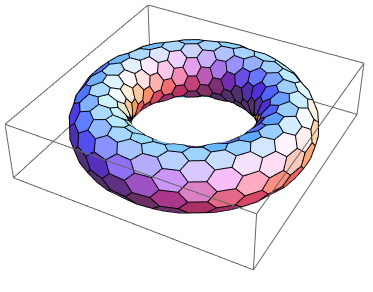
\includegraphics[width=0.75\textwidth]{images/test_image}
	\caption{Current Balance in a Tokamak} ~\\
	\small In a tokamak, there needs to be a certain amount of current -- and that current has to come from somewhere. All good reactors have an adequate bootstrap current. What provides the remaining current is what distinguishes steady state from pulsed operation.
	\label{fig:curbal}
\end{figure}

This equation shows how steady-state and pulsed operation can coexist (see \cref{fig:curbal}). The final point to make is reducing the model to being purely pulsed -- i.e.\ neglecting the current drive:
\begin{equation}
	1 = f_{BS} + f_{ID}
\end{equation}
Therefore, the next chapter will generalize the steady current to allow pulsed operation, and then simplify it to the purely pulsed case. Just as steady current faced self-consistency issues with $\eta_{CD}$, this current will also involve its own root solving conundrum -- the description of which will be given in the following two chapters.

\subsubsection{The Tokamak Magnet Strength -- $B_0$}

The tokamak magnet strength has no \replaced{unique}{obvious} equation to eliminate it. With foresight, the one this model \replaced{uses}{chooses to use} is \added{the} power balance \replaced{inherent to every}{in a} reactor. Similar to current balance, power balance is what separates a reactor from a \replaced{device incapable of producing net electricity}{toaster}. As such, it is referred throughout this document as: the primary constraint. It will be derived later this chapter.

\subsubsection{The Tokamak Major Radius -- $R_0$}

Much like the magnet strength, the major radius has no \replaced{unique}{obvious} relation to express it. \replaced{The model therefore uses this equation to handle a reactor's various}{This is convenient, because the model still has yet to resolve one of its most pressing issues:} physical and engineering-based constraints. This \deleted{laundry} list of requirements further restricts reactor space to the curves shown in the results section. Collectively, these are referred to as the \replaced{limiting}{secondary} constraints -- discussed later this chapter. \replaced{These}{By miracle, these} constraints all just happen to depend on the size of the reactor -- the reason they are chosen to \replaced{represent}{substitute out} the radius.

\section{Enforcing Power Balance}

What separates a reactor from a \replaced{device incapable of producing net electricity}{toaster} is power balance. \replaced{Within a tokamak, it}{It} accounts for how the power going into a plasma's core exactly matches the power coming out of it. To approximate this conservation equation, two sets of power will be introduced: the sources and the sinks. 

The sources have mainly been introduced at this point -- they include the alpha power ($P_\alpha$) \added{from fusion reactions} and the heating power ($P_H$), as well as a new ohmic power term ($P_\Omega$). The remaining two powers -- the sinks -- then appear through the radiation and heat conduction losses, which will be given shortly. In equation form, power balance becomes:
\begin{equation}
	\sum_{sources} P = \sum_{sinks} \, P
\end{equation}
or expanded to fit this model:
\begin{equation}
	\label{eq:power_balance}
	P_\alpha + P_H + P_\Omega = P_{BR} + P_\kappa
\end{equation}
For clarity, the left-hand side of this equality are the sources. Whereas the remaining two are sinks, i.e.\ Bremsstrahlung radiation ($P_{BR}$) and heat conduction losses ($P_\kappa$).

\subsection{Collecting Power Sources}

As suggested, the two dominant sources of power in a tokamak are: alpha power ($P_\alpha$) and auxiliary heating ($P_H$). From \cref{chapter:power}, it was determined that alpha particles (i.e.\ helium nuclei) carry around 20\% of the total fusion power; or as we put it mathematically:
\begin{equation}
	\label{eq:palpha}
	P_\alpha = \frac{P_F}{5}
\end{equation}
Additionally, it was determined that the heating power is what was eventually amplified into fusion power -- or through equation:
\begin{equation}
	\label{eq:ph}
	P_H = \frac{P_F}{Q}
\end{equation}
The final source term then is the ohmic power ($P_\Omega$). This is identical to how copper wires in a home heat up as current runs through them. From a simple circuits picture, the power across the plasma is related to its current and resistance -- in our standardized units -- through:
\begin{equation}
	\label{eq:pohmic_basic}
	P_\Omega = 10^6 \cdot I_P^2 \cdot R_P
\end{equation}
\deleted{Here, the resistance of the plasma is unlike any material humans encounter on a daily basis -- actually decreasing with temperature.} \replaced{This}{The} fusion systems model handles the plasma resistance ($R_P$)  with the neoclassical Spitzer resistivity. Through equation,\added{\cite{jeff}}
\begin{equation}
	\label{eq:rp}
	R_P = \frac{K_{RP}}{R_0 \overline T ^ {3/2}}
\end{equation}
\begin{equation}
	K_{RP} = 5.6e{-8} \cdot \left( \frac{ Z_{eff} }{ \epsilon^2 \kappa } \right) \cdot \left( \frac{1}{ 1 - 1.31 \sqrt{ \epsilon } + 0.46 \epsilon } \right)
\end{equation}

Combined with the Greenwald limit, ohmic power can be written more compactly as,
\begin{equation}
	\label{eq:pohmic}
	P_\Omega = K_\Omega \cdot \left( \frac{ \overline n ^ 2 R_0^3 }{\overline T ^ {3/2}} \right)
\end{equation}
\begin{equation}
	K_\Omega = 10^6 \cdot \frac{K_{RP}}{K_n^2}
\end{equation}
With the sources defined, we are now in a position to discuss the two sink terms used in this model's power balance.

\subsection{Approximating Radiation Losses}

All nuclear reactors emit radiation. From a power balance perspective, this means some power has to always be reserved to recoup from its losses -- measured in megawatts. In a fusion reactor, the three most important types of radiation are: Bremsstrahlung radiation, line radiation, and synchrotron radiation. 

\replaced{This}{Without going into too much detail, this} model chooses to only model Bremsstrahlung radiation -- as it usually dominates within the plasma's core. \added{Within most designs, Bremsstrahlung radiation outweighs the other two's contribution, to core power balance, two-to-one.\cite{ussteady,inputfile} } However, adding the effects of line-radiation and synchrotron radiation would drive results closer to real-world experiments. For example, line-radiation would better account for the \added{effects of} heavy impurities that \replaced{are emitted from the divertor plate and first wall}{appear as pieces of a tokamak fall into the plasma.}

For clarity, Bremsstrahlung -- or breaking -- radiation is what occurs when a charged particle (e.g.\ an electron) is accelerated by some means. In a tokamak, this happens all the time as \replaced{electrons collide with the ion species.\cite{hutch}}{charged particles are flung around and around the machine.} \replaced{This term can be}{As given in Jeff Freidberg's book, this term is} described by the volume integral:\added{\cite{jeff}}
\begin{equation}
	P_{BR} = \int S_{BR} \, d \vec{r}
\end{equation}

\replaced{Where}{Here,} the radiation power density ($S_{BR}$) is given by:
\begin{equation}
	S_{BR} = \left( \frac{\sqrt{2}}{3 \sqrt{\pi^5}} \cdot \frac{e^6}{\epsilon_0^2 c^3 h m_e^{3/2}} \right) \cdot \left( Z_{eff} \, n^2 \, T^{1/2} \right)
\end{equation}

The constants in the left set of parentheses all have their usual physics meanings (i.e.\ c is the speed of light and $m_e$ is the mass of an electron). What is new is the effective charge: $Z_{eff}$.

The effective charge is a scheme for \replaced{reducing}{collapsing} the charge \replaced{each ion}{that each particle} has to a \replaced{single representative}{collective} value. Fundamental charge, here, is what: neutrons lack, electrons and hydrogen have one of, and helium has two. As such, a plasma with a purely deuterium and tritium fuel would have an effective charge of one. This value would then quickly rise if a Tungsten tile -- with 74 units of charge -- were to fall into the plasma core from the walls of the tokamak.

Using the volume integral -- seen in the derivation of fusion power -- allows the Bremsstrahlung power to be written in standardized units as:
\begin{equation}
	\label{eq:pbr}
	P_{BR} = K_{BR} \ \overline n ^ 2 \ \overline T ^ {1/2} R_0^3 
\end{equation}
\begin{equation}
	K_{BR} = 0.1056 \, \frac{ (1+\nu_n)^2 \, (1+\nu_T)^{1/2} }{1+2 \, \nu_n + 0.5 \, \nu_T} \, Z_{eff} \, \epsilon^2 \, \kappa \, g
\end{equation}

This power term represents the radiation power losses involved in power balance. All that is needed now is a formula for heat conduction losses -- \replaced{one of the most difficult plasma behaviors}{the hardest plasma behavior} to model to date.

\subsection{Estimating Heat Conduction Losses}

Heat is energy that \replaced{moves about randomly}{lacks direction} on a microscopic level. Macroscopically, it generally moves from hotter areas to colder ones. As hinted by the plasma profile for temperature, heat emanates from the center of a plasma and migrates towards the walls of its tokamak enclosure. It therefore \replaced{is a critical}{seems an important} quantity to calculate when balancing power in a plasma's core.

The difficulty of estimating heat conduction, though, lies in the \replaced{nonlinear behaviors}{chaotic nature} of plasmas -- no theory or \replaced{quick-running code}{computation today} can properly model it. As such, reactor designers have turned towards experimentalists for empirical scaling laws based on the dozen or so strongest tokamaks in the world. These are collectively referred to as confinement time scalings, i.e.\ the ELMy H-Mode Scaling Law.

The derivation of this heat conduction loss term ($P_\kappa$) starts in a manner similar to the previous powers. To begin, an equation for $P_\kappa$ \replaced{can be found using the following volume integral:\cite{jeff}}{sis given in Jeff Freidberg's book as:} 
\begin{equation}
	P_\kappa = \frac{1}{\tau_E} \int U d \vec r
\end{equation}

This volume integral includes two new terms: the confinement time ($\tau_E$) and the internal energy (U). Before explaining these terms, a qualitative description is in order. As mentioned previously, the heat -- or microscopically random -- energy is captured by the internal energy (U). Then the confinement time ($\tau_E$) is how long it would take for the heat to \replaced{undergo an e-folding}{completely leave the device} if the \replaced{device}{system} were suddenly turned off.

A formula for confinement time will be delayed till the end of this section, when it is needed to solve for the magnetic field ($B_0$). The internal energy (U), however, can be given now as it has its typical physics meaning. This assumes that all three plasma species are held nearly at the same temperature (T) as the electrons:
\begin{equation}
	U = \frac{3}{2} \left( n + n_D + n_T \right) T
\end{equation}

Here again, $n_D$ and $n_T$ -- the density of deuterium and tritium, respectively -- are related to the electron density (used in this model) through the dilution factor, which assumes a 50-50 mix of D-T fuel:
\begin{equation}
	n_D = n_T = f_D \cdot \left( \, \frac{n}{2} \, \right)
\end{equation}

\replaced{After several substitutions,}{Foregoing the mathematical rigor of previous sections,} the equations here can be combined to form an equation for $P_\kappa$ -- the heat conduction losses -- in standardized units:
\begin{equation}
	\label{eq:pkappa}
	P_\kappa = K_\kappa \, \frac{ R_0 ^ 3 \ \overline{n}  \ \overline{T}  }{\tau_E} 
\end{equation}
\begin{equation}
	K_\kappa = 0.4744 \, ( 1 + f_D ) \, \frac{ (1 + \nu_n) \, (1 + \nu_T) }{1 + \nu_n + \nu_T } \, ( \, \epsilon^2 \, \kappa \, g \, )
\end{equation}

Now that all five terms have been defined in power balance, the next step is expanding it and solving for the tokamak's toroidal magnetic field strength: $B_0$.

\subsection{Writing the Lawson \replaced{Parameter}{Criterion}}

Before \replaced{arriving at a formula for}{locking in the primary constraint -- i.e.\ } the magnet strength ($B_0$) \replaced{using}{equation from} power \replaced{balance,}{balance} -- it seems appropriate to take a detour and explain an intermediate solution: the Lawson \replaced{Parameter}{Criterion}. Within the fusion community, the Lawson \replaced{Parameter}{Criterion} is the cornerstone in any argument on the possibility of a \replaced{tokamak ever}{design} being used as a \replaced{reactor.}{reactor (and not just some grandiose toaster).}

An equation for the Lawson \replaced{Parameter}{Criterion} -- sometimes referred to as the \emph{triple product} -- is easily found in the literature as:
\begin{equation}
	\label{eq:lawson}
	n \cdot T \cdot \tau_E = \frac{ 60 }{ E_F } \cdot \frac{ T ^ 2 }{ \langle \sigma v \rangle }
\end{equation}

Similar to the steady current derived earlier, the right-hand side is only dependent on temperature. Further, as the left-hand side is a measure of difficult to achieve parameters, the goal is to minimize both sides. \replaced{As shown in \cref{fig:lawson}, this}{This} occurs when the plasma temperature is around 15 keV -- a fact \replaced{well known to}{memorized by} many fusion engineers. As will be seen, this is a simplified result of our model. This is why $\overline T$ = 15 keV is not always the optimum temperature -- but usually is in the right neighborhood for reasonable reactor designs.

\begin{figure}
	\centering
	\begin{adjustbox}{width=0.75\textwidth}
		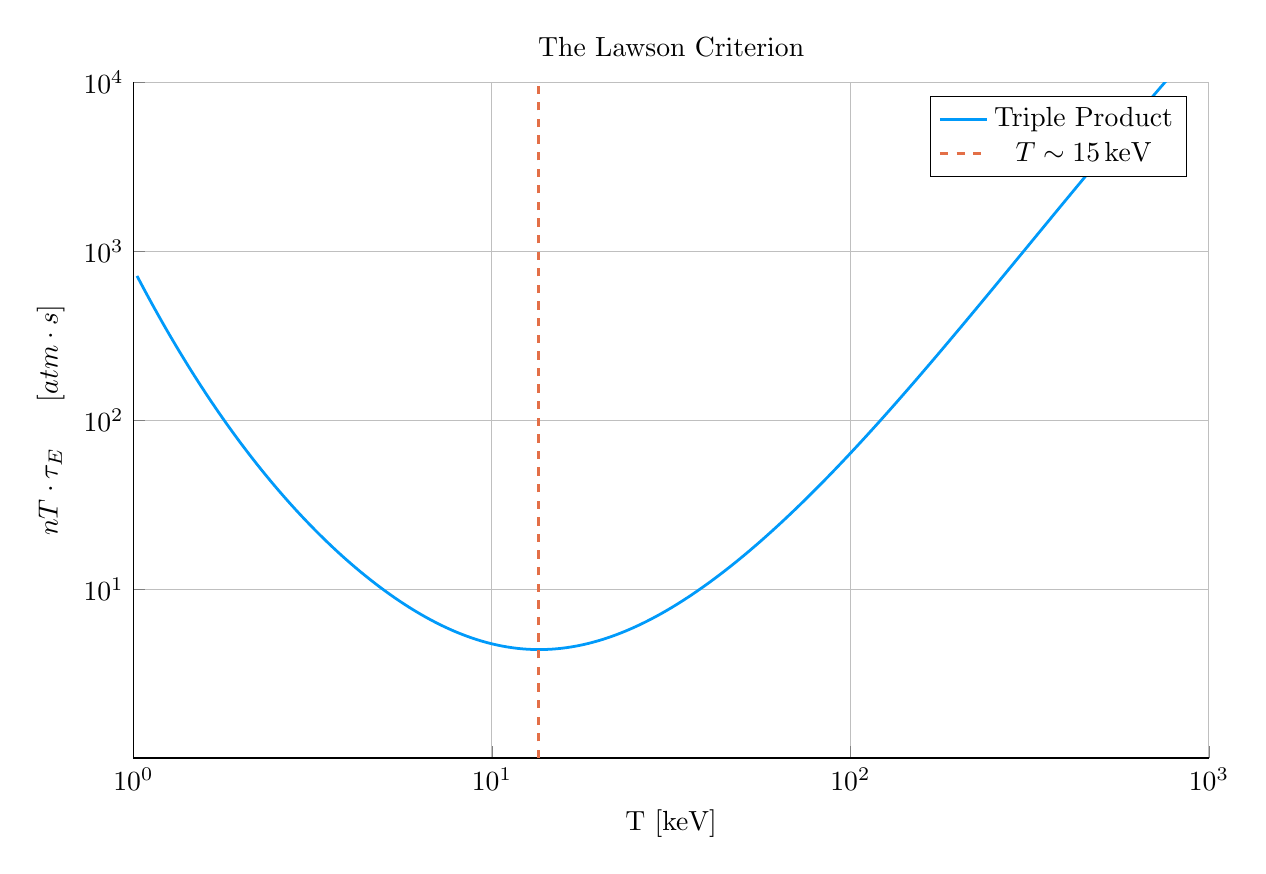
\begin{tikzpicture}[]
\begin{axis}[height = {101.6mm}, ylabel = {$n T \cdot \tau_E \ \ \ \ \ [atm \cdot s]$}, title = {The Lawson Criterion}, xmin = {1.0}, xmax = {1000.0}, ymax = {10000.0}, ymode = {log}, xlabel = {T   [keV]}, {unbounded coords=jump, xticklabel style={rotate = 0}, log basis x=10, xmajorgrids = true, xtick = {1.0,10.0,100.0,1000.0}, xticklabels = {$10^{0}$,$10^{1}$,$10^{2}$,$10^{3}$}, xtick align = inside, axis lines* = left, yticklabel style={rotate = 0}, log basis y=10, ymajorgrids = true, ytick = {10.0,100.0,1000.0,10000.0}, yticklabels = {$10^{1}$,$10^{2}$,$10^{3}$,$10^{4}$}, ytick align = inside, axis lines* = left,     xshift = 0.0mm,
    yshift = 0.0mm,
    axis background/.style={fill={rgb,1:red,1.00000000;green,1.00000000;blue,1.00000000}}
}, xmode = {log}, ymin = {1.001}, width = {152.4mm}]\addplot+ [color = {rgb,1:red,0.00000000;green,0.60560316;blue,0.97868012},
draw opacity=1.0,
line width=1,
solid,mark = none,
mark size = 2.0,
mark options = {
    color = {rgb,1:red,0.00000000;green,0.00000000;blue,0.00000000}, draw opacity = 1.0,
    fill = {rgb,1:red,0.00000000;green,0.60560316;blue,0.97868012}, fill opacity = 1.0,
    line width = 1,
    rotate = 0,
    solid
}]coordinates {
(1.023292992280754, 715.5843693055245)
(1.0471285480508996, 652.0764819850596)
(1.0715193052376064, 594.8592282501459)
(1.096478196143185, 543.2546522451097)
(1.1220184543019633, 496.663131536487)
(1.1481536214968828, 454.5537705698688)
(1.1748975549395295, 416.456035426309)
(1.202264434617413, 381.9524618339787)
(1.2302687708123816, 350.67229211863474)
(1.2589254117941673, 322.2859170225961)
(1.288249551693134, 296.50001561571264)
(1.318256738556407, 273.0533013093717)
(1.3489628825916535, 251.71279464231827)
(1.3803842646028848, 232.27055435304894)
(1.4125375446227544, 214.54080755655357)
(1.4454397707459274, 198.35742783107645)
(1.4791083881682074, 183.57171688596867)
(1.5135612484362082, 170.05045138851656)
(1.5488166189124815, 157.67416161454238)
(1.5848931924611136, 146.33561297294165)
(1.62181009735893, 135.9384652384002)
(1.6595869074375607, 126.3960875950959)
(1.6982436524617444, 117.63051042010802)
(1.7378008287493754, 109.57149718083319)
(1.7782794100389228, 102.155721939162)
(1.8197008586099834, 95.32603979193581)
(1.8620871366628675, 89.03083917128589)
(1.9054607179632472, 83.22346631314609)
(1.9498445997580451, 77.86171340616474)
(1.9952623149688795, 72.90736298097448)
(2.041737944669529, 68.32578201236458)
(2.0892961308540396, 64.08556000253319)
(2.137962089502232, 60.158186007840044)
(2.1877616239495525, 56.51776017780416)
(2.2387211385683394, 53.14073590510077)
(2.290867652767773, 50.0056891489945)
(2.344228815319922, 47.093111900666955)
(2.3988329190194904, 44.38522711472284)
(2.4547089156850306, 41.86582274326229)
(2.51188643150958, 39.52010278288166)
(2.5703957827688635, 37.33455348568332)
(2.6302679918953817, 35.29682309703734)
(2.6915348039269156, 33.395613669101465)
(2.7542287033381663, 31.62058366316803)
(2.8183829312644537, 29.962260198507185)
(2.884031503126606, 28.411959932944896)
(2.9512092266663856, 26.961717673034713)
(3.019951720402016, 25.60422191119189)
(3.0902954325135905, 24.332756575143232)
(3.1622776601683795, 23.141148352912094)
(3.2359365692962827, 22.0237190255119)
(3.311311214825911, 20.975242300634317)
(3.3884415613920256, 19.990904694824255)
(3.4673685045253166, 19.066270059743925)
(3.548133892335755, 18.197247390865947)
(3.630780547701014, 17.380061594923447)
(3.715352290971725, 16.611226926240565)
(3.8018939632056115, 15.887522832148305)
(3.890451449942806, 15.205971974493213)
(3.9810717055349722, 14.563820218135483)
(4.073802778041127, 13.9585183986498)
(4.168693834703354, 13.387705700467096)
(4.265795188015927, 12.849194493696395)
(4.36515832240166, 12.340956493058842)
(4.466835921509632, 11.86111011596177)
(4.570881896148751, 11.407908928906801)
(4.677351412871983, 10.979731082327069)
(4.786300923226384, 10.575069643717114)
(4.897788193684462, 10.192523747682124)
(5.011872336272722, 9.830790489396893)
(5.1286138399136485, 9.4886574950276)
(5.248074602497725, 9.16499610901522)
(5.370317963702527, 8.858755143826464)
(5.495408738576246, 8.568955142911767)
(5.623413251903491, 8.29468311223238)
(5.7543993733715695, 8.035087679882023)
(5.88843655355589, 7.789374647081937)
(6.025595860743578, 7.556802897213308)
(6.165950018614822, 7.336680632605374)
(6.309573444801933, 7.1283619115573345)
(6.456542290346556, 6.931243460563939)
(6.606934480075959, 6.7447617389697925)
(6.760829753919817, 6.5683902353161425)
(6.918309709189364, 6.4016369764913525)
(7.079457843841379, 6.244042232468866)
(7.244359600749901, 6.095176400934137)
(7.413102413009175, 5.954638057478739)
(7.5857757502918375, 5.822052158290098)
(7.762471166286917, 5.697068383402136)
(7.943282347242816, 5.579359609605691)
(8.128305161640993, 5.4686205030596)
(8.31763771102671, 5.364566222501177)
(8.511380382023766, 5.266931224738075)
(8.709635899560805, 5.175468164818683)
(8.912509381337454, 5.089946883932297)
(9.120108393559097, 5.010153478689247)
(9.33254300796991, 4.93588944597961)
(9.549925860214358, 4.866970898113729)
(9.772372209558107, 4.803227843409827)
(10.0, 4.74450352782116)
(10.232929922807541, 4.690653833587014)
(10.471285480508996, 4.641546731255455)
(10.715193052376065, 4.597061781760152)
(10.964781961431852, 4.557089685544928)
(11.220184543019636, 4.521531876017525)
(11.481536214968829, 4.490300154882151)
(11.748975549395297, 4.463316367150074)
(12.02264434617413, 4.4405121138606)
(12.302687708123818, 4.4218285007630715)
(12.589254117941675, 4.407215921415124)
(12.882495516931343, 4.39663387334517)
(13.182567385564074, 4.390050806109046)
(13.489628825916533, 4.38744400024263)
(13.803842646028846, 4.388799476276163)
(14.12537544622754, 4.3941119331320175)
(14.454397707459272, 4.403384715376948)
(14.791083881682072, 4.416629808943959)
(15.13561248436208, 4.433867865077917)
(15.488166189124811, 4.455128252393695)
(15.848931924611133, 4.48044913706814)
(16.218100973589298, 4.509877591315835)
(16.595869074375607, 4.5434697304270015)
(16.982436524617444, 4.581290878772013)
(17.378008287493753, 4.6234157653040935)
(17.78279410038923, 4.669928749218003)
(18.197008586099834, 4.72092407655112)
(18.620871366628677, 4.7765061686425785)
(19.054607179632473, 4.836789943498778)
(19.498445997580454, 4.9019011712485865)
(19.952623149688797, 4.971976865010962)
(20.417379446695296, 5.047165708641305)
(20.892961308540396, 5.127628522971638)
(21.379620895022324, 5.213538772314609)
(21.87761623949553, 5.305083113162599)
(22.3872113856834, 5.4024619871819475)
(22.908676527677734, 5.505890260779421)
(23.442288153199225, 5.615597913703399)
(23.9883291901949, 5.73183077933847)
(24.547089156850298, 5.854851339557513)
(25.118864315095795, 5.984939577213792)
(25.703957827688633, 6.122393889584756)
(26.302679918953814, 6.267532066323497)
(26.915348039269155, 6.420692335730828)
(27.542287033381662, 6.582234483434617)
(28.183829312644534, 6.752541047852738)
(28.84031503126606, 6.932018597123181)
(29.512092266663856, 7.121099092511616)
(30.19951720402016, 7.3202413436533345)
(30.902954325135905, 7.52993256135462)
(31.622776601683793, 7.750690014070107)
(32.359365692962825, 7.983062794588698)
(33.11311214825911, 8.227633703902626)
(33.884415613920254, 8.485021259704226)
(34.673685045253166, 8.75588183745494)
(35.48133892335755, 9.040911952501903)
(36.30780547701014, 9.340850692282585)
(37.15352290971726, 9.656482308258274)
(38.018939632056124, 9.988638977855283)
(38.90451449942807, 10.33820374737135)
(39.810717055349734, 10.706113667526031)
(40.73802778041128, 11.093363134099329)
(41.68693834703355, 11.50100744691819)
(42.65795188015925, 11.930166601314705)
(43.65158322401658, 12.382029327098968)
(44.6683592150963, 12.857857391065538)
(45.708818961487495, 13.358990180088743)
(46.77351412871981, 13.886849582961755)
(47.86300923226383, 14.442945190302456)
(48.97788193684461, 15.028879833087446)
(50.11872336272722, 15.646355481690618)
(51.28613839913648, 16.297179528695864)
(52.48074602497726, 16.983271480232325)
(53.70317963702527, 17.706670082146438)
(54.954087385762456, 18.469540908986364)
(56.23413251903491, 19.274184445531887)
(57.543993733715695, 20.1230446924667)
(58.8843655355589, 21.01871832976149)
(60.25595860743578, 21.963964473423015)
(61.65950018614822, 22.96171506347328)
(63.09573444801933, 24.015085923357283)
(64.56542290346556, 25.127388533447483)
(66.06934480075961, 26.302142563921986)
(67.60829753919819, 27.543089215049925)
(69.18309709189366, 28.85420541582856)
(70.79457843841381, 30.2397189349887)
(72.44359600749902, 31.704124461627565)
(74.13102413009177, 33.25220071614717)
(75.85775750291836, 34.889028655780834)
(77.62471166286916, 36.620010842788844)
(79.43282347242814, 38.45089204740532)
(81.2830516164099, 40.387781161829686)
(83.17637711026708, 42.43717450598852)
(85.11380382023764, 44.6059806104552)
(87.09635899560806, 46.90154656681403)
(89.12509381337455, 49.331686040906135)
(91.20108393559097, 51.90470904980014)
(93.3254300796991, 54.62945360900688)
(95.49925860214358, 57.515319362410956)
(97.72372209558107, 60.57230331363601)
(100.0, 63.81103778410115)
(102.32929922807536, 67.24283072987917)
(104.71285480508996, 70.87970855663967)
(107.1519305237606, 74.73446157946178)
(109.64781961431851, 78.82069228215158)
(112.2018454301963, 83.15286653889214)
(114.81536214968828, 87.74636796962139)
(117.48975549395291, 92.61755560946783)
(120.22644346174131, 97.78382508189834)
(123.02687708123811, 103.26367347494983)
(125.89254117941675, 109.07676813004912)
(128.82495516931337, 115.24401956346287)
(131.82567385564073, 121.78765875140567)
(134.89628825916532, 128.7313190212372)
(138.03842646028852, 136.10012280306256)
(141.2537544622754, 143.92077350836064)
(144.5439770745928, 152.22165281508785)
(147.91083881682073, 161.03292365197024)
(151.35612484362088, 170.38663918850096)
(154.88166189124811, 180.3168581514265)
(158.48931924611142, 190.859766803331)
(162.18100973589299, 202.05380793424246)
(165.95869074375614, 213.93981723308698)
(169.82436524617444, 226.5611674222155)
(173.78008287493762, 239.96392055525848)
(177.82794100389228, 254.19698889610504)
(181.97008586099827, 269.3123048150095)
(186.20871366628674, 285.3650001565748)
(190.54607179632464, 302.41359555379074)
(194.98445997580455, 320.5202001823509)
(199.52623149688787, 339.75072247016425)
(204.17379446695296, 360.175092298409)
(208.92961308540387, 381.86749525252964)
(213.79620895022325, 404.9066195044671)
(218.77616239495518, 429.37591593094083)
(223.872113856834, 455.36387209705316)
(229.08676527677724, 482.9643007596241)
(234.42288153199226, 512.2766435708044)
(239.88329190194898, 543.4062906894171)
(245.4708915685031, 576.464917035484)
(251.18864315095797, 611.5708359522358)
(257.03957827688646, 648.8493710699868)
(263.02679918953817, 688.4332471972791)
(269.1534803926917, 730.4630010970918)
(275.4228703338166, 775.087413039401)
(281.8382931264455, 822.4639600564246)
(288.40315031266056, 872.7592918631268)
(295.1209226666387, 926.1497304436313)
(301.9951720402016, 982.8217943436637)
(309.0295432513592, 1042.972748750622)
(316.22776601683796, 1106.8111824860716)
(323.5936569296281, 1174.5576130809143)
(331.1311214825911, 1246.4451211509213)
(338.84415613920237, 1322.7200153403764)
(346.73685045253166, 1403.6425291540393)
(354.8133892335753, 1489.4875510528248)
(363.0780547701014, 1580.545389247023)
(371.5352290971724, 1677.1225726820153)
(380.1893963205613, 1779.542689776586)
(389.04514499428046, 1888.147266542193)
(398.1071705534973, 2003.2966857842675)
(407.3802778041126, 2125.3711491630897)
(416.8693834703355, 2254.771683973346)
(426.57951880159254, 2391.92119658728)
(436.5158322401661, 2537.2655745980082)
(446.683592150963, 2691.2748397961623)
(457.0881896148752, 2854.4443542162185)
(467.73514128719813, 3027.296081597634)
(478.6300923226385, 3210.379906722357)
(489.77881936844614, 3404.2750152128565)
(501.18723362727246, 3609.591336506103)
(512.8613839913648, 3826.971052857308)
(524.8074602497728, 4057.0901773752544)
(537.0317963702527, 4300.660204247052)
(549.5408738576248, 4558.429834477045)
(562.341325190349, 4831.186780640399)
(575.4399373371566, 5119.759654339896)
(588.843655355589, 5425.019940252352)
(602.5595860743575, 5747.884060862276)
(616.5950018614822, 6089.315536203627)
(630.957344480193, 6450.327243166718)
(645.6542290346556, 6831.983779178804)
(660.6934480075957, 7235.403935331275)
(676.0829753919819, 7661.763284308377)
(691.8309709189363, 8112.296888768487)
(707.945784384138, 8588.302136144339)
(724.4359600749899, 9091.141706159546)
(741.3102413009177, 9622.24667771128)
(758.5775750291835, 10183.11978213795)
(776.247116628692, 10775.338810284076)
(794.3282347242813, 11400.560181185736)
(812.8305161640995, 12060.52268063764)
(831.7637711026708, 12757.051378360826)
(851.1380382023768, 13492.06173297636)
(870.9635899560806, 14267.563894499495)
(891.2509381337459, 15085.667214609008)
(912.0108393559096, 15948.584975511469)
(933.2543007969915, 16858.63934881972)
(954.992586021436, 17818.266596491703)
(977.2372209558112, 18830.022526540524)
(1000.0, 19896.588216921093)
(1023.2929922807537, 21020.77602173607)
(1047.1285480508996, 22205.535874673045)
(1071.519305237606, 23453.961905400487)
(1096.4781961431852, 24769.29938550517)
(1122.018454301963, 26154.952021453166)
(1148.1536214968828, 27614.489613007096)
(1174.897554939529, 29151.656096526574)
(1202.2644346174131, 30770.37799363245)
(1230.268770812381, 32474.77328681697)
(1258.9254117941675, 34269.16074474929)
(1288.2495516931335, 36158.06972124623)
(1318.2567385564075, 38146.2504531722)
(1348.9628825916532, 40238.68488388557)
(1380.3842646028852, 42440.598040283076)
(1412.537544622754, 44757.46999299408)
(1445.439770745928, 47195.048430870826)
(1479.1083881682073, 49759.3618825815)
(1513.5612484362086, 52456.73361988538)
(1548.816618912481, 55293.79627901266)
(1584.893192461114, 58277.5072385393)
(1621.8100973589299, 61415.16479419626)
(1659.5869074375614, 64714.42517323727)
(1698.2436524617442, 68183.3204332687)
(1737.8008287493763, 71830.27729287352)
(1778.2794100389228, 75664.13694389607)
(1819.7008586099826, 79694.17589795444)
(1862.0871366628676, 83930.12792257269)
(1905.4607179632462, 88382.20712532024)
(1949.8445997580454, 93061.13224750487)
(1995.2623149688789, 97978.15223228547)
(2041.7379446695295, 103145.07313560059)
(2089.296130854039, 108574.28645200086)
(2137.9620895022326, 114278.79893140584)
(2187.761623949552, 120272.26396692236)
(2238.72113856834, 126569.01463824147)
(2290.8676527677726, 133184.09849971998)
(2344.228815319923, 140133.3142071364)
(2398.83291901949, 147433.25008222583)
(2454.708915685031, 155101.32471954415)
(2511.88643150958, 163155.82974591767)
(2570.3957827688646, 171615.97484880453)
(2630.2679918953813, 180501.9351962624)
(2691.5348039269165, 189834.9013779866)
(2754.2287033381663, 199637.13200398907)
(2818.382931264455, 209932.00910503615)
(2884.031503126606, 220744.09648690396)
(2951.209226666387, 232099.20119892008)
(3019.9517204020162, 244024.43828613157)
(3090.295432513592, 256548.29900382337)
(3162.2776601683795, 269700.72268301074)
(3235.936569296281, 283513.1724460091)
(3311.311214825911, 298018.714982234)
(3388.441561392024, 313252.1046060778)
(3467.368504525317, 329249.87183106877)
(3548.133892335753, 346050.41670754453)
(3630.780547701014, 363694.1071848948)
(3715.352290971724, 382223.3827739712)
(3801.8939632056126, 401682.863800698)
(3890.4514499428046, 422119.46655815904)
(3981.0717055349733, 443582.52468168386)
(4073.802778041126, 466123.9170895939)
(4168.693834703355, 489798.2028515374)
(4265.795188015925, 514662.763366615)
(4365.158322401661, 540777.9522550126)
(4466.835921509631, 568207.2533895164)
(4570.881896148751, 597017.4475173334)
(4677.351412871981, 627278.7879479581)
(4786.300923226385, 659065.1858096905)
(4897.7881936844615, 692454.4054057244)
(5011.872336272725, 727528.2702307551)
(5128.613839913648, 764372.8802406823)
(5248.074602497728, 803078.841001585)
(5370.317963702527, 843741.5053794787)
(5495.408738576249, 886461.2284699624)
(5623.413251903491, 931343.6365063301)
(5754.399373371566, 978499.910526803)
(5888.43655355589, 1.0280470856256834e6)
(6025.595860743575, 1.080108366660198e6)
(6165.9500186148225, 1.1348134613343545e6)
(6309.57344480193, 1.1922989316334699e6)
(6456.542290346556, 1.252708564638612e6)
(6606.934480075957, 1.3161937638086632e6)
(6760.829753919818, 1.3829139618799328e6)
(6918.309709189362, 1.4530370565986685e6)
(7079.457843841381, 1.52673987057139e6)
(7244.359600749898, 1.6042086365912505e6)
(7413.102413009177, 1.6856395098764265e6)
(7585.775750291836, 1.771239108738555e6)
(7762.4711662869195, 1.8612250852863907e6)
(7943.282347242814, 1.955826727861547e6)
(8128.305161640995, 2.0552855970008024e6)
(8317.63771102671, 2.1598561968221436e6)
(8511.380382023768, 2.2698066838408946e6)
(8709.635899560806, 2.385419615337356e6)
(8912.509381337459, 2.506992739519579e6)
(9120.108393559096, 2.6348398298537624e6)
(9332.543007969914, 2.7692915660716193e6)
(9549.92586021436, 2.910696464508343e6)
(9772.372209558112, 3.0594218605781165e6)
(10000.0, 3.2158549463557494e6)
};
\addlegendentry{Triple Product}
\addplot+ [color = {rgb,1:red,0.88887350;green,0.43564919;blue,0.27812294},
draw opacity=1.0,
line width=1,
dashed,mark = none,
mark size = 2.0,
mark options = {
    color = {rgb,1:red,0.00000000;green,0.00000000;blue,0.00000000}, draw opacity = 1.0,
    fill = {rgb,1:red,0.88887350;green,0.43564919;blue,0.27812294}, fill opacity = 1.0,
    line width = 1,
    rotate = 0,
    solid
}]coordinates {
(13.489628825916533, 1.0)
(13.489628825916533, 10000.0)
};
\addlegendentry{$T \sim 15 \, \textnormal{keV}$}
\end{axis}

\end{tikzpicture}

	\end{adjustbox}
%	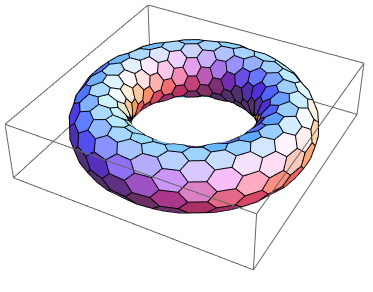
\includegraphics[width=0.75\textwidth]{images/test_image}
	\caption{Power Balance in a Reactor} ~\\
	\small Power balance is what differentiates a reactor from a radiator. When cast as the Lawson \replaced{Parameter}{Criterion} for fusion, it explains why D-T plasmas often have a temperature around 15 keV.
	\label{fig:lawson}
\end{figure}

As all the terms in power balance have already been defined, the starting point will be simply repeating the standardized equations for all five included powers.
\begin{equation}
	\tag{\ref{eq:palpha}}
	P_\alpha = \frac{P_F}{5}
\end{equation}
\begin{equation}
	\tag{\ref{eq:ph}}
	P_H = \frac{P_F}{Q}
\end{equation}
\begin{equation}
	\tag{\ref{eq:pohmic}}
	P_\Omega = K_\Omega \cdot \left( \frac{ \overline n ^ 2 R_0^3 }{\overline T ^ {3/2}} \right)
\end{equation}
\begin{equation}
	\tag{\ref{eq:pbr}}
	P_{BR} = K_{BR} \ \overline n ^ 2 \ \overline T ^ {1/2} R_0^3 
\end{equation}
\begin{equation}
	\tag{\ref{eq:pkappa}}
	P_\kappa = K_\kappa \, \frac{ R_0 ^ 3 \ \overline{n}  \ \overline{T}  }{\tau_E} 
\end{equation}

With the fusion power again being,
\begin{equation}
	\tag{\ref{eq:pf}}
	P_F = K_F \cdot \overline{n}^2 \cdot R_0^3  \cdot (\sigma v)
\end{equation}
These can then be substituted into power balance:
\begin{equation}
	\tag{\ref{eq:power_balance}}
	P_\alpha + P_H + P_\Omega = P_{BR} + P_\kappa
\end{equation}
After a couple lines of algebra, power balance can be rewritten in a form analogous to the triple product:
\begin{equation}
	\label{eq:ntaue}
	 \overline{n}  \cdot \overline{T} \cdot \tau_E = \frac{ K_\kappa \, \overline{T}^{\,2} }{ \left( K_P \, (\sigma v) +  K_{OH} \, \overline{T}^{  \,-3/2 } \right) - K_{BR} \, \overline{T}^{  \,1/2 } }
\end{equation}
\begin{equation}
	K_P = K_F \cdot \left( \frac{5 + Q}{5 \times Q} \right)
\end{equation}
\replaced{As expected, this shares a form}{As can be seen, this is remarkably} similar to the simple Lawson \replaced{Parameter}{Criterion}:
\begin{equation}
	\tag{\ref{eq:lawson}}
	n \cdot T \cdot \tau_E = \frac{ 60 }{ E_F } \cdot \frac{ T ^ 2 }{ \langle \sigma v \rangle }
\end{equation} 
The main difference is this model does not ignore ohmic power and radiation losses completely. The inclusion of radiation for example sometimes bars a range of temperatures from being physically realizable.\footnote{ The denominator of Eq \ref{eq:ntaue} has discontinuities when the $K_{BR} \, \overline{T}^{  \,1/2 }$ term exactly equals the parenthesised one. Therefore, valid reactors only exist outside the discontinuities, when the entire triple product is finite and positive. } With this intermediate relation in place, the goal is now to give a formula for the confinement time and solve it for the magnetic field strength ($B_0$) -- thus giving the Primary Constraint.

\subsection{Finalizing the Primary Constraint}

The goal now is to transform the Lawson \replaced{Parameter}{Criterion} into an equation for magnet strength ($B_0$). This choice to solve the equation for $B_0$ was \replaced{motivated by the goals of analysis and how it will fit}{completely arbitrary, only motivated by the foresight of how it fits} into the fusion systems model. To solve the primary constraint, the confinement time scaling law will need to be introduced. At the end, a \replaced{convoluted}{messy} -- albeit highly useful -- relation will be the reward.

The energy confinement time -- $\tau_E$ -- is one of the most \replaced{difficult to obtain}{elusive} terms in all of fusion energy. It is an attempt to \replaced{reduce}{boil down} all the \replaced{nonlinear behaviors}{chaotic nature} of plasmas into a simple measure of how fast its internal energy would be ejected from the tokamak if the device was instantaneously shut down. As such, reactor designers have turned toward experimentalists for empirical scalings based on the world's tokamaks. These all share a form similar to:
\begin{equation}
	\tau_E = K_\tau \, H \, \frac{
		I_P^{\,\alpha_I} \, R_0^{\,\alpha_R} \, a^{\,\alpha_a} \, \kappa^{\,\alpha_\kappa} \ \overline{n}^{\,\alpha_n} \, B_0^{\,\alpha_B} \, A^{\,\alpha_A}
	}{ P_{src} ^ {\,\alpha_P} }
	\label{eq:tau_gen}
\end{equation}
This \replaced{regressional fit}{mouthful of a formula} is how the field actually designs machines (i.e.\ ITER). Let it be known, though, that \replaced{fits of this kind}{these fits} often do remarkable well, having relative errors less than 20\% on interpolated data. The new terms in this equation are: $P_{src}$, $K_\tau$, H, A, and the $\alpha_{\,\square}$ factors. 

First, the loss power is a metric used in the engineering community to quantify the power being transported out of the ``core'' of the plasma by charged particles (i.e.\ not the neutrons). \cite{process} To optimize fits, experimentalists have defined this as a combination of the source power terms:
\begin{equation}
	\label{eq:pl}
	P_{src} = P_\alpha + P_H + P_\Omega
\end{equation}
\deleted{However, many have argued that the term should actually be replaced by its correct physics meaning -- the conductive heat loss power. As this model uses the ELMy H-Mode scaling law, which is standard in the field, this alternative definition will not be used:}
%\begin{equation}
%	\tilde P_{src} \approx P_\kappa = P_\alpha + P_H + P_\Omega - P_{BR}
%\end{equation}
Moving on, $K_\tau$ is simply a constant fit-makers use in their scalings. Whereas H is the \replaced{enhancement factor over the empirical fit.}{(H-Mode) scaling factor -- the analogue of $K_\tau$ used by reactor designers. This H factor can be used to artificially boost the confinement of a machine (i.e.\ it adds a little bit of magic).} \replaced{Next,}{Continuing,} A is the average mass number of the fuel source, in atomic mass units. For a 50-50 D-T fuel, this is 2.5, as deuterium weighs two amus and tritium weighs three. Lastly, the alpha factors (e.g.\ $\alpha_n$, $\alpha_a$, $\alpha_P$) are fitting parameters that represent each variable's relative importance in the scaling. 

For ELMy H-Mode, this confinement scaling law can be written as:
\begin{equation}
	\tau_E = 0.145 \, H \, \frac{
		I_P^{0.93} \, R_0^{1.39} \, a^{0.58} \, \kappa^{0.78} \ \overline{n}^{\, 0.41} \, B_0^{0.15} \, A^{0.19}
	}{ P_{src} ^ {\,0.69} }
	\label{eq:tau_h}
\end{equation}
\replaced{However, similar scaling laws}{Where similar ones} can be \replaced{written}{given} for L-Mode, I-Mode, etc. One final remark to make before moving on is that even these fits have subtleties. The value of $\kappa$, for example, may have a slightly different geometric meaning from tokamak to tokamak. And the exact definition of loss power -- $P_{src}$ -- introduces an even larger area of discrepancy.  \deleted{Although not actually used, a better fit for our model might be one from the author:}
%\begin{equation}
%	\tilde \tau_E = 0.08 \, H \frac{  
%		\left( R_0^{1.49} B_0 ^ {0.3} I_P^{0.93} \right) \cdot \left( \epsilon ^ {0.17} A^{0.23}  \kappa ^ {0.56} \right) }{ \tilde P_{src} ^ {\, 0.54} }	
%\end{equation}

Returning to the problem at hand, though, this model's Lawson \replaced{Parameter}{Criterion} (eq. \ref{eq:ntaue}) can be simplified after expanding the left-hand side using the Greenwald density and substituting in a confinement time scaling law. \replaced{After a few lines of algebra, this can be transformed}{Albeit a little cumbersome, this can be wrangled} into \replaced{a formula}{an equation} for $B_0$!
\begin{equation}
	\label{eq:b_0_power}
	\tcbhighmath{
	B_0 = \left( \frac{ G_{PB} }{ K_{PB} } \cdot \left( I_P^{\,\alpha_I^*} \, R_0^{ \alpha_R^* } \right)^{-1} \right) ^ { \frac{1}{ \alpha_B } }
	}
\end{equation}
\begin{equation}
	G_{PB} = \frac{ \overline{T} \cdot \left( \, K_P (\sigma v) + K_\Omega  \, \overline{T}^{  \,-3/2 } \, \right) ^ { \alpha_P } }{ \left( \, K_P (\sigma v) + K_\Omega  \, \overline{T}^{  \,-3/2 } - K_{BR} \, \overline{T}^{  \,1/2 } \, \right) }
\end{equation}
\begin{equation}
	K_{PB} = H \cdot \left( \frac{ K_\tau K_n^{\alpha_n^*}}{K_\kappa } \right) \cdot \left( 
     \epsilon^{\,\alpha_a} \, \kappa^{\,\alpha_\kappa} \, A^{\,\alpha_A}\right)
\end{equation}

Where we have added new starred alpha values for the density, current, and major radius:
\begin{equation}
  \alpha_n^* = 1 + \alpha_n - 2 \alpha_P
\end{equation}
\begin{equation}
  \alpha_I^* = \alpha_I + \alpha_n^*
\end{equation}
\begin{equation}
  \alpha_R^* = \alpha_R + \alpha_a - 2  \alpha_n^* - 3 \alpha_p
\end{equation}

\deleted{Again, if the alternate definition for heat loss ($\tilde P_{abs}$) were used, another definition for $G_{PB}$ would arise. Quickly reemphasizing, though, these tilded values are not actually used in the model:}
%\begin{equation}
%	\tilde G_{PB} = \frac{ \overline{T} }{ \left( \, K_P (\sigma v) + K_\Omega  \, \overline{T}^{  \,-3/2 } - K_{BR} \, \overline{T}^{  \,1/2 } \, \right) ^ { ( 1 - \alpha_P ) } }
%\end{equation}

This equation for $B_0$ -- derived from power balance -- is thus the primary constraint for reactor designs. It is the first step in connecting the plasma (i.e.\ $\overline n$, $\overline T$, and $I_P$) to its tokamak enclosure (i.e.\ $B_0$ and $R_0$). The remaining step is finding an equation -- or in this case, equations -- for the major radius of the device. These radius equations will collectively be referred to as: the \replaced{limiting constraints.}{Secondary Constraints.}

%\subsection{Exploring the Freidberg Criterion}

\deleted{Before moving onto the Secondary Constraint, it is worth noting that this power balance equation can be written in a triple product form analogous to the Lawson \replaced{Parameter}{Criterion}. For this reason, we will refer to it as the Freidberg Triple Product:}
%\begin{equation}
%	\label{eq:freidberg}
%	R_0^{ \alpha_R^* } \cdot B_0^{\,\alpha_B} \cdot I_P^{\,\alpha_I^*} = \frac{ G_{PB} }{ K_{PB} }
%\end{equation}

%\begin{figure*}[h]
%    \centering
%    \hfill 
%    \begin{subfigure}[t]{0.45\textwidth}
%        \centering
%		\begin{adjustbox}{width=\textwidth}
%			\Large
%			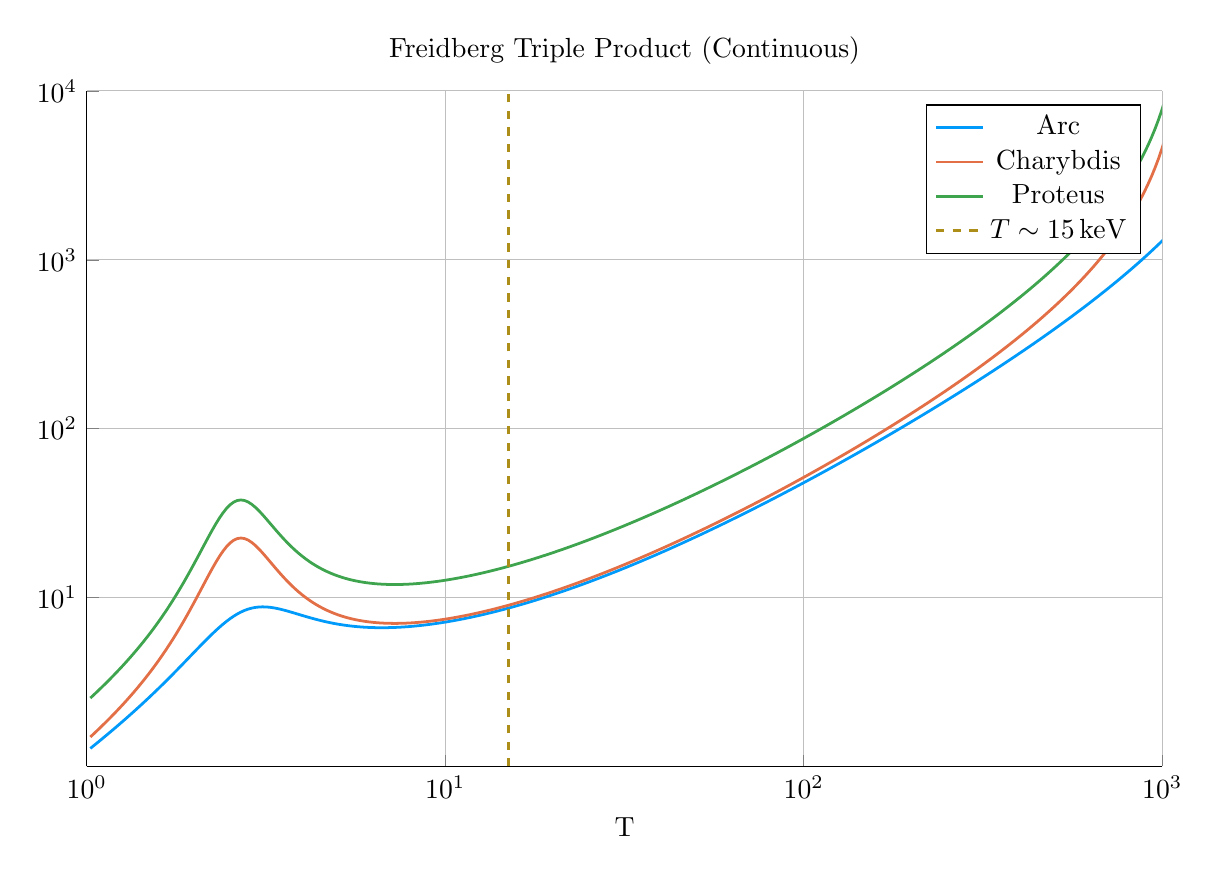
\begin{tikzpicture}[]
\begin{axis}[height = {101.6mm}, ylabel = {}, title = {Freidberg Triple Product (Continuous)}, xmin = {1.0}, xmax = {1000.0}, ymax = {10000.0}, ymode = {log}, xlabel = {T}, {unbounded coords=jump, xticklabel style={rotate = 0}, log basis x=10, xmajorgrids = true, xtick = {1.0,10.0,100.0,1000.0}, xticklabels = {$10^{0}$,$10^{1}$,$10^{2}$,$10^{3}$}, xtick align = inside, axis lines* = left, yticklabel style={rotate = 0}, log basis y=10, ymajorgrids = true, ytick = {10.0,100.0,1000.0,10000.0}, yticklabels = {$10^{1}$,$10^{2}$,$10^{3}$,$10^{4}$}, ytick align = inside, axis lines* = left,     xshift = 0.0mm,
    yshift = 0.0mm,
    axis background/.style={fill={rgb,1:red,1.00000000;green,1.00000000;blue,1.00000000}}
}, xmode = {log}, ymin = {1.001}, width = {152.4mm}]\addplot+ [color = {rgb,1:red,0.00000000;green,0.60560316;blue,0.97868012},
draw opacity=1.0,
line width=1,
solid,mark = none,
mark size = 2.0,
mark options = {
    color = {rgb,1:red,0.00000000;green,0.00000000;blue,0.00000000}, draw opacity = 1.0,
    fill = {rgb,1:red,0.00000000;green,0.60560316;blue,0.97868012}, fill opacity = 1.0,
    line width = 1,
    rotate = 0,
    solid
}]coordinates {
(1.023292992280754, 1.2793221218652944)
(1.0471285480508996, 1.3309195883591072)
(1.0715193052376064, 1.3850036910515204)
(1.096478196143185, 1.4417288746419747)
(1.1220184543019633, 1.5012617022690462)
(1.1481536214968828, 1.5637819142077942)
(1.1748975549395295, 1.6294835657026674)
(1.202264434617413, 1.698576242531264)
(1.2302687708123816, 1.7712863496330842)
(1.2589254117941673, 1.8478584635873476)
(1.288249551693134, 1.928556733480841)
(1.318256738556407, 2.0136663062561424)
(1.3489628825916535, 2.103494741323413)
(1.3803842646028848, 2.1983733642456036)
(1.4125375446227544, 2.2986584896716016)
(1.4454397707459274, 2.4047324181909375)
(1.4791083881682074, 2.5170040789980095)
(1.5135612484362082, 2.635909148564986)
(1.5488166189124815, 2.7619094231676584)
(1.5848931924611136, 2.8954911583354357)
(1.62181009735893, 3.0371620095937497)
(1.6595869074375607, 3.1874461154129454)
(1.6982436524617444, 3.3468767556900265)
(1.7378008287493754, 3.515985900410607)
(1.7782794100389228, 3.6952898405140475)
(1.8197008586099834, 3.8852699797335295)
(1.8620871366628675, 4.08634778460181)
(1.9054607179632472, 4.298852874384422)
(1.9498445997580451, 4.5229833332653655)
(1.9952623149688795, 4.758757610889229)
(2.041737944669529, 5.005957927860106)
(2.0892961308540396, 5.264066012456858)
(2.137962089502232, 5.532193347327445)
(2.1877616239495525, 5.809009942726736)
(2.2387211385683394, 6.092677927494796)
(2.290867652767773, 6.380798757486339)
(2.344228815319922, 6.670385163416938)
(2.3988329190194904, 6.957870427901035)
(2.4547089156850306, 7.239167326284057)
(2.51188643150958, 7.509786194163538)
(2.5703957827688635, 7.7650155007458315)
(2.6302679918953817, 8.000159131951143)
(2.6915348039269156, 8.210813513493981)
(2.7542287033381663, 8.393157056383407)
(2.8183829312644537, 8.544217197329235)
(2.884031503126606, 8.662079281751163)
(2.9512092266663856, 8.746008028642427)
(3.019951720402016, 8.796465438819597)
(3.0902954325135905, 8.815025707881876)
(3.1622776601683795, 8.80420376037562)
(3.2359365692962827, 8.767225560018067)
(3.311311214825911, 8.707773161635059)
(3.3884415613920256, 8.629735524841195)
(3.4673685045253166, 8.536989174977906)
(3.548133892335755, 8.433223490199008)
(3.630780547701014, 8.32181619294888)
(3.715352290971725, 8.205757228033434)
(3.8018939632056115, 8.087614356783817)
(3.890451449942806, 7.9695314352280215)
(3.9810717055349722, 7.853249952422453)
(4.073802778041127, 7.740145297390103)
(4.168693834703354, 7.631270787751151)
(4.265795188015927, 7.527404208691776)
(4.36515832240166, 7.429093260768431)
(4.466835921509632, 7.33669764878841)
(4.570881896148751, 7.250426597707905)
(4.677351412871983, 7.170371324123017)
(4.786300923226384, 7.096532487933503)
(4.897788193684462, 7.028842950140937)
(5.011872336272722, 6.967186322975986)
(5.1286138399136485, 6.911411862292244)
(5.248074602497725, 6.861346254119733)
(5.370317963702527, 6.816802812809654)
(5.495408738576246, 6.777588554906853)
(5.623413251903491, 6.743509552318662)
(5.7543993733715695, 6.714374907663976)
(5.88843655355589, 6.689999637968835)
(6.025595860743578, 6.670206702159046)
(6.165950018614822, 6.654828363817934)
(6.309573444801933, 6.643707043377312)
(6.456542290346556, 6.636695782809513)
(6.606934480075959, 6.633658420300284)
(6.760829753919817, 6.634469551553204)
(6.918309709189364, 6.63901433757021)
(7.079457843841379, 6.6471882052930455)
(7.244359600749901, 6.658896476780433)
(7.413102413009175, 6.674053954122599)
(7.5857757502918375, 6.692584480627425)
(7.762471166286917, 6.714420493592822)
(7.943282347242816, 6.7395025799146895)
(8.128305161640993, 6.767779042630784)
(8.31763771102671, 6.79920548407566)
(8.511380382023766, 6.833744409466334)
(8.709635899560805, 6.871364853329812)
(8.912509381337454, 6.9120420301239145)
(9.120108393559097, 6.955757009615049)
(9.33254300796991, 7.002496416999287)
(9.549925860214358, 7.0522521573385)
(9.772372209558107, 7.105021163593507)
(10.0, 7.160805167339729)
(10.232929922807541, 7.2196104911458425)
(10.471285480508996, 7.281447861469827)
(10.715193052376065, 7.346332241007961)
(10.964781961431852, 7.41428267931583)
(11.220184543019636, 7.485322180621463)
(11.481536214968829, 7.559477587761894)
(11.748975549395297, 7.6367794812276)
(12.02264434617413, 7.7172620923547175)
(12.302687708123818, 7.800963229763945)
(12.589254117941675, 7.887924218206006)
(12.882495516931343, 7.978189849034269)
(13.182567385564074, 8.071808341585202)
(13.489628825916533, 8.168831314805496)
(13.803842646028846, 8.26931376852079)
(14.12537544622754, 8.373314073794269)
(14.454397707459272, 8.480893971874206)
(14.791083881682072, 8.592118581277306)
(15.13561248436208, 8.707056412599798)
(15.488166189124811, 8.825779390690416)
(15.848931924611133, 8.948362883858978)
(16.218100973589298, 9.074885739831279)
(16.595869074375607, 9.205430328195467)
(16.982436524617444, 9.340082589117413)
(17.378008287493753, 9.478932088132577)
(17.78279410038923, 9.622072076850081)
(18.197008586099834, 9.769599559430906)
(18.620871366628677, 9.921615364726758)
(19.054607179632473, 10.07822422398916)
(19.498445997580454, 10.239534854079999)
(19.952623149688797, 10.405660046135063)
(20.417379446695296, 10.576716759651381)
(20.892961308540396, 10.752826221987263)
(21.379620895022324, 10.9341140332813)
(21.87761623949553, 11.120710276812883)
(22.3872113856834, 11.312749634842634)
(22.908676527677734, 11.510371509986186)
(23.442288153199225, 11.7137201521892)
(23.9883291901949, 11.922944791385861)
(24.547089156850298, 12.138199775936432)
(25.118864315095795, 12.359644716953252)
(25.703957827688633, 12.587444638637452)
(26.302679918953814, 12.821770134761826)
(26.915348039269155, 13.062797531448128)
(27.542287033381662, 13.310709056400045)
(28.183829312644534, 13.565693014765834)
(28.84031503126606, 13.82794397181769)
(29.512092266663856, 14.097662942647972)
(30.19951720402016, 14.375057589095706)
(30.902954325135905, 14.660342424130278)
(31.622776601683793, 14.953739023932986)
(32.359365692962825, 15.25547624793148)
(33.11311214825911, 15.565790467056377)
(33.884415613920254, 15.884925800504542)
(34.673685045253166, 16.213134361308995)
(35.48133892335755, 16.550676511031238)
(36.30780547701014, 16.8978211239089)
(37.15352290971726, 17.254845860808384)
(38.018939632056124, 17.622037453350618)
(38.90451449942807, 17.999691998596774)
(39.810717055349734, 18.38811526470027)
(40.73802778041128, 18.78762300795229)
(41.68693834703355, 19.198541301669295)
(42.65795188015925, 19.6212068773937)
(43.65158322401658, 20.05596748532388)
(44.6683592150963, 20.503182229545445)
(45.708818961487495, 20.963222013454047)
(46.77351412871981, 21.436469871175646)
(47.86300923226383, 21.923321410447826)
(48.97788193684461, 22.424185232528163)
(50.11872336272722, 22.939483374951877)
(51.28613839913648, 23.469651771317768)
(52.48074602497726, 24.015140728856327)
(53.70317963702527, 24.576415424552575)
(54.954087385762456, 25.153956420636177)
(56.23413251903491, 25.748260200293693)
(57.543993733715695, 26.35983972450207)
(58.8843655355589, 26.989225010929704)
(60.25595860743578, 27.636963735901347)
(61.65950018614822, 28.303621860475566)
(63.09573444801933, 28.989784281739404)
(64.56542290346556, 29.69605551048393)
(66.06934480075961, 30.423060376486795)
(67.60829753919819, 31.171444762694403)
(69.18309709189366, 31.941876369666343)
(70.79457843841381, 32.735045511719214)
(72.44359600749902, 33.55166594628614)
(74.13102413009177, 34.39247573809195)
(75.85775750291836, 35.25823815983267)
(77.62471166286916, 36.14974263114321)
(79.43282347242814, 37.06780569773617)
(81.2830516164099, 38.013272052702476)
(83.17637711026708, 38.98701560207701)
(85.11380382023764, 39.989940581159736)
(87.09635899560806, 41.02298269407601)
(89.12509381337455, 42.08711036866879)
(91.20108393559097, 43.18332598001413)
(93.3254300796991, 44.312667194688736)
(95.49925860214358, 45.476208349136186)
(97.72372209558107, 46.675061895023376)
(100.0, 47.910379911219174)
(102.32929922807536, 49.1833556845266)
(104.71285480508996, 50.49522536463268)
(107.1519305237606, 51.84726969599379)
(109.64781961431851, 53.24081583131803)
(112.2018454301963, 54.67723923102123)
(114.81536214968828, 56.15796565338645)
(117.48975549395291, 57.684473240449044)
(120.22644346174131, 59.258294704948604)
(123.02687708123811, 60.88101962402365)
(125.89254117941675, 62.55429684569091)
(128.82495516931337, 64.27983701453458)
(131.82567385564073, 66.05941522345191)
(134.89628825916532, 67.89487379874117)
(138.03842646028852, 69.78812522630338)
(141.2537544622754, 71.74115522723595)
(144.5439770745928, 73.75602599165504)
(147.91083881682073, 75.83487958017014)
(151.35612484362088, 77.97994150307832)
(154.88166189124811, 80.19352448802711)
(158.48931924611142, 82.47803244763931)
(162.18100973589299, 84.83596466314262)
(165.95869074375614, 87.2699201708478)
(169.82436524617444, 89.7826024444658)
(173.78008287493762, 92.3768242568097)
(177.82794100389228, 95.05551286856803)
(181.97008586099827, 97.82171548255974)
(186.20871366628674, 100.6786050083681)
(190.54607179632464, 103.62948615355889)
(194.98445997580455, 106.67780186293392)
(199.52623149688787, 109.82714012887666)
(204.17379446695296, 113.08124119760298)
(208.92961308540387, 116.44400519767774)
(213.79620895022325, 119.91950022156021)
(218.77616239495518, 123.51197088641831)
(223.872113856834, 127.2258474138247)
(229.08676527677724, 131.06575526002374)
(234.42288153199226, 135.0365253375378)
(239.88329190194898, 139.14320487005486)
(245.4708915685031, 143.39106892630025)
(251.18864315095797, 147.785632682383)
(257.03957827688646, 152.33266446627786)
(263.02679918953817, 157.03819964265176)
(269.1534803926917, 161.908555401256)
(275.4228703338166, 166.9503465175865)
(281.8382931264455, 172.1705021605638)
(288.40315031266056, 177.57628382861546)
(295.1209226666387, 183.175304502876)
(301.9951720402016, 188.97554911427625)
(309.0295432513592, 194.98539643459995)
(316.22776601683796, 201.21364248106408)
(323.5936569296281, 207.66952561997678)
(331.1311214825911, 214.36275345331575)
(338.84415613920237, 221.30353162896512)
(346.73685045253166, 228.50259481386476)
(354.8133892335753, 235.97123994530904)
(363.0780547701014, 243.7213619906034)
(371.5352290971724, 251.7654924325556)
(380.1893963205613, 260.11684072588844)
(389.04514499428046, 268.78933899522207)
(398.1071705534973, 277.7976902739334)
(407.3802778041126, 287.1574206152656)
(416.8693834703355, 296.88493544311495)
(426.57951880159254, 306.99758055039047)
(436.5158322401661, 317.51370819846284)
(446.683592150963, 328.45274882261293)
(457.0881896148752, 339.83528890503925)
(467.73514128719813, 351.6831556525324)
(478.6300923226385, 364.019509161591)
(489.77881936844614, 376.86894288507557)
(501.18723362727246, 390.25759326505363)
(512.8613839913648, 404.2132595327318)
(524.8074602497728, 418.76553479281586)
(537.0317963702527, 433.94594965392275)
(549.5408738576248, 449.78812983073925)
(562.341325190349, 466.32796933763944)
(575.4399373371566, 483.6038210717674)
(588.843655355589, 501.65670694780766)
(602.5595860743575, 520.5305498494844)
(616.5950018614822, 540.2724301816861)
(630.957344480193, 560.9328700805296)
(645.6542290346556, 582.566148886756)
(660.6934480075957, 605.2306538385934)
(676.0829753919819, 628.989270851766)
(691.8309709189363, 653.90982069593)
(707.945784384138, 680.0655469086195)
(724.4359600749899, 707.5356627471048)
(741.3102413009177, 736.4059656912784)
(758.5775750291835, 766.7695294432701)
(776.247116628692, 798.727485079221)
(794.3282347242813, 832.3899050561196)
(812.8305161640995, 867.8768062379246)
(831.7637711026708, 905.319291075073)
(851.1380382023768, 944.8608496698408)
(870.9635899560806, 986.6588498377013)
(891.2509381337459, 1030.8862476245677)
(912.0108393559096, 1077.7335573068228)
(933.2543007969915, 1127.411128001834)
(954.992586021436, 1180.1517840590136)
(977.2372209558112, 1236.213898917512)
(1000.0, 1295.8849878014776)
(1023.2929922807537, 1359.4859243956064)
(1047.1285480508996, 1427.3759117201514)
(1071.519305237606, 1499.9583694362552)
(1096.4781961431852, 1577.687940957739)
(1122.018454301963, 1661.0788770147035)
(1148.1536214968828, 1750.7151218116257)
(1174.897554939529, 1847.262519332875)
(1202.2644346174131, 1951.4836786284711)
(1230.268770812381, 2064.2561993145287)
(1258.9254117941675, 2186.595178121113)
(1288.2495516931335, 2319.6812176589965)
(1318.2567385564075, 2464.8955729365553)
(1348.9628825916532, 2623.864652612861)
(1380.3842646028852, 2798.516914142382)
(1412.537544622754, 2991.1563761807724)
(1445.439770745928, 3204.5587002127395)
(1479.1083881682073, 3442.098361225498)
(1513.5612484362086, 3707.9193124396793)
(1548.816618912481, 4007.1675479581536)
(1584.893192461114, 4346.313439566653)
(1621.8100973589299, 4733.607058236353)
(1659.5869074375614, 5179.735215473649)
(1698.2436524617442, 5698.792798685391)
(1737.8008287493763, 6309.758994188134)
(1778.2794100389228, 7038.813610830222)
(1819.7008586099826, 7923.109724291594)
(1862.0871366628676, 9017.195901992123)
(1905.4607179632462, 10404.546791614655)
(1949.8445997580454, 12219.667076115855)
(1995.2623149688789, 14694.120959228087)
(2041.7379446695295, 18263.35087394861)
(2089.296130854039, 23854.381911656048)
(2137.9620895022326, 33852.2908799337)
(2187.761623949552, 56824.35846897241)
(2238.72113856834, 164426.65765500255)
(2290.8676527677726, -199130.5391041138)
(2344.228815319923, -63592.36702962983)
(2398.83291901949, -38401.823826757456)
(2454.708915685031, -27793.602877328278)
(2511.88643150958, -21952.016301942476)
(2570.3957827688646, -18256.558428890912)
(2630.2679918953813, -15710.129369983011)
(2691.5348039269165, -13850.495487055317)
(2754.2287033381663, -12434.055966251428)
(2818.382931264455, -11320.247131391827)
(2884.031503126606, -10422.274535612401)
(2951.209226666387, -9683.646906144215)
(3019.9517204020162, -9066.01284792254)
(3090.295432513592, -8542.595957682206)
(3162.2776601683795, -8093.376345071255)
(3235.936569296281, -7704.429898465926)
(3311.311214825911, -7364.644013312067)
(3388.441561392024, -7065.587403461628)
(3467.368504525317, -6800.6560221766695)
(3548.133892335753, -6564.6034987731455)
(3630.780547701014, -6353.209298630934)
(3715.352290971724, -6163.039676144607)
(3801.8939632056126, -5991.272496174683)
(3890.4514499428046, -5835.566864306992)
(3981.0717055349733, -5693.964740791021)
(4073.802778041126, -5564.815743424234)
(4168.693834703355, -5446.719003997193)
(4265.795188015925, -5338.477730561384)
(4365.158322401661, -5239.0633500512895)
(4466.835921509631, -5147.586954620055)
(4570.881896148751, -5063.276373046262)
(4677.351412871981, -4985.457615476961)
(4786.300923226385, -4913.539746969296)
(4897.7881936844615, -4847.002480006052)
(5011.872336272725, -4785.385915699954)
(5128.613839913648, -4728.282033811321)
(5248.074602497728, -4675.327569873742)
(5370.317963702527, -4626.198049926041)
(5495.408738576249, -4580.602740941166)
(5623.413251903491, -4538.280376245746)
(5754.399373371566, -4498.995513494782)
(5888.43655355589, -4462.535419726061)
(6025.595860743575, -4428.7073965916015)
(6165.9500186148225, -4397.336474861534)
(6309.57344480193, -4368.26342005518)
(6456.542290346556, -4341.343001287243)
(6606.934480075957, -4316.442483667796)
(6760.829753919818, -4293.440311248033)
(6918.309709189362, -4272.224953180315)
(7079.457843841381, -4252.693889506939)
(7244.359600749898, -4234.752717844742)
(7413.102413009177, -4218.314364047006)
(7585.775750291836, -4203.29838315304)
(7762.4711662869195, -4189.630338739936)
(7943.282347242814, -4177.241250766746)
(8128.305161640995, -4166.067102901534)
(8317.63771102671, -4156.048402374031)
(8511.380382023768, -4147.1297856871)
(8709.635899560806, -4139.259664786595)
(8912.509381337459, -4132.389908913949)
(9120.108393559096, -4126.475558010264)
(9332.543007969914, -4121.474564078605)
(9549.92586021436, -4117.347557371377)
(9772.372209558112, -4114.057634664823)
(10000.0, -4111.57016722244)
};
\addlegendentry{Arc}
\addplot+ [color = {rgb,1:red,0.88887350;green,0.43564919;blue,0.27812294},
draw opacity=1.0,
line width=1,
solid,mark = none,
mark size = 2.0,
mark options = {
    color = {rgb,1:red,0.00000000;green,0.00000000;blue,0.00000000}, draw opacity = 1.0,
    fill = {rgb,1:red,0.88887350;green,0.43564919;blue,0.27812294}, fill opacity = 1.0,
    line width = 1,
    rotate = 0,
    solid
}]coordinates {
(1.023292992280754, 1.4951205905179736)
(1.0471285480508996, 1.564933213170644)
(1.0715193052376064, 1.6391186292624738)
(1.096478196143185, 1.7180622084543624)
(1.1220184543019633, 1.8021941616786232)
(1.1481536214968828, 1.8919958608612342)
(1.1748975549395295, 1.9880071734245173)
(1.202264434617413, 2.0908349882404913)
(1.2302687708123816, 2.2011631409423815)
(1.2589254117941673, 2.3197639825513616)
(1.288249551693134, 2.4475118764272956)
(1.318256738556407, 2.5853989543987748)
(1.3489628825916535, 2.7345535126429543)
(1.3803842646028848, 2.896261479310555)
(1.4125375446227544, 3.0719914348155988)
(1.4454397707459274, 3.263423704587518)
(1.4791083881682074, 3.472484060035992)
(1.5135612484362082, 3.7013825352091754)
(1.5488166189124815, 3.952657759716108)
(1.5848931924611136, 4.229226968304124)
(1.62181009735893, 4.534441388686033)
(1.6595869074375607, 4.872145900529501)
(1.6982436524617444, 5.2467405015013435)
(1.7378008287493754, 5.663238917158036)
(1.7782794100389228, 6.127316227593624)
(1.8197008586099834, 6.645332071138777)
(1.8620871366628675, 7.224308067533204)
(1.9054607179632472, 7.871826706510841)
(1.9498445997580451, 8.595803300518865)
(1.9952623149688795, 9.404062589508452)
(2.041737944669529, 10.303628945858334)
(2.0892961308540396, 11.29961963663557)
(2.137962089502232, 12.393627534998426)
(2.1877616239495525, 13.581517950512376)
(2.2387211385683394, 14.850682342251654)
(2.290867652767773, 16.177033787448202)
(2.344228815319922, 17.522414780403594)
(2.3988329190194904, 18.833549197849237)
(2.4547089156850306, 20.04397470378986)
(2.51188643150958, 21.08013836114596)
(2.5703957827688635, 21.871665671436986)
(2.6302679918953817, 22.36384995966289)
(2.6915348039269156, 22.528612673585403)
(2.7542287033381663, 22.369948558667186)
(2.8183829312644537, 21.921824163906248)
(2.884031503126606, 21.23964003953929)
(2.9512092266663856, 20.38872623352358)
(3.019951720402016, 19.433663321546106)
(3.0902954325135905, 18.430838621774875)
(3.1622776601683795, 17.424807209897704)
(3.2359365692962827, 16.44773839121447)
(3.311311214825911, 15.520762283244057)
(3.3884415613920256, 14.656147043575608)
(3.4673685045253166, 13.859584188165677)
(3.548133892335755, 13.132200852217746)
(3.630780547701014, 12.47216002027133)
(3.715352290971725, 11.875847565048533)
(3.8018939632056115, 11.33870683093359)
(3.890451449942806, 10.855798600216186)
(3.9810717055349722, 10.42215943225786)
(4.073802778041127, 10.033018273423268)
(4.168693834703354, 9.683916918667496)
(4.265795188015927, 9.370767350264446)
(4.36515832240166, 9.089869055571175)
(4.466835921509632, 8.837902043453784)
(4.570881896148751, 8.6119060006025)
(4.677351412871983, 8.409252359661203)
(4.786300923226384, 8.227613555065604)
(4.897788193684462, 8.064932075325121)
(5.011872336272722, 7.91939082590377)
(5.1286138399136485, 7.789385611127785)
(5.248074602497725, 7.673500098221017)
(5.370317963702527, 7.570483353424563)
(5.495408738576246, 7.479229879408585)
(5.623413251903491, 7.398761994753704)
(5.7543993733715695, 7.328214353551413)
(5.88843655355589, 7.266820388638273)
(6.025595860743578, 7.213900464232118)
(6.165950018614822, 7.168851535440971)
(6.309573444801933, 7.131138128615018)
(6.456542290346556, 7.100284474923121)
(6.606934480075959, 7.075867648120776)
(6.760829753919817, 7.057511575241371)
(6.918309709189364, 7.0448818053617135)
(7.079457843841379, 7.03768093643693)
(7.244359600749901, 7.035644614021524)
(7.413102413009175, 7.0385380224948895)
(7.5857757502918375, 7.046152816528243)
(7.762471166286917, 7.058304415490602)
(7.943282347242816, 7.074829633505994)
(8.128305161640993, 7.095584590601089)
(8.31763771102671, 7.120442873022589)
(8.511380382023766, 7.149293910866733)
(8.709635899560805, 7.182041545986132)
(8.912509381337454, 7.218602766766122)
(9.120108393559097, 7.258906589488317)
(9.33254300796991, 7.30289306863743)
(9.549925860214358, 7.350512420953691)
(9.772372209558107, 7.401724249797036)
(10.0, 7.456496858332535)
(10.232929922807541, 7.514806641813107)
(10.471285480508996, 7.576637547200618)
(10.715193052376065, 7.641980601233738)
(10.964781961431852, 7.710833485482428)
(11.220184543019636, 7.7832001671752655)
(11.481536214968829, 7.859090571781095)
(11.748975549395297, 7.93852029572274)
(12.02264434617413, 8.02151035478933)
(12.302687708123818, 8.108086964714632)
(12.589254117941675, 8.198281350809156)
(12.882495516931343, 8.292129583902065)
(13.182567385564074, 8.38967244017214)
(13.489628825916533, 8.490955282751791)
(13.803842646028846, 8.596027963097924)
(14.12537544622754, 8.704944740753675)
(14.454397707459272, 8.817764219656572)
(14.791083881682072, 8.934549299966482)
(15.13561248436208, 9.055367144163561)
(15.488166189124811, 9.180289156424717)
(15.848931924611133, 9.309390974391308)
(16.218100973589298, 9.442752472549282)
(16.595869074375607, 9.580457776539694)
(16.982436524617444, 9.722595287804594)
(17.378008287493753, 9.869257717974659)
(17.78279410038923, 10.020542133007641)
(18.197008586099834, 10.176550005569382)
(18.620871366628677, 10.337387276815504)
(19.054607179632473, 10.50316442620314)
(19.498445997580454, 10.673996549542666)
(19.952623149688797, 10.850003445038157)
(20.417379446695296, 11.031309707177495)
(20.892961308540396, 11.21804482837071)
(21.379620895022324, 11.410343308360655)
(21.87761623949553, 11.608344770822882)
(22.3872113856834, 11.81219408853973)
(22.908676527677734, 12.02204151524775)
(23.442288153199225, 12.238042826008586)
(23.9883291901949, 12.460359464612567)
(24.547089156850298, 12.689158699600375)
(25.118864315095795, 12.924613787966877)
(25.703957827688633, 13.166904147140388)
(26.302679918953814, 13.41621553534255)
(26.915348039269155, 13.672740240532336)
(27.542287033381662, 13.936677278161076)
(28.183829312644534, 14.208232597989184)
(28.84031503126606, 14.487619300239052)
(29.512092266663856, 14.775057861382548)
(30.19951720402016, 15.070776369886339)
(30.902954325135905, 15.37501077226307)
(31.622776601683793, 15.688005129802471)
(32.359365692962825, 16.010011886382863)
(33.11311214825911, 16.341292147791066)
(33.884415613920254, 16.68211597300732)
(34.673685045253166, 17.03276267794145)
(35.48133892335755, 17.39352115213756)
(36.30780547701014, 17.764690188997083)
(37.15352290971726, 18.146578830103802)
(38.018939632056124, 18.539506724270478)
(38.90451449942807, 18.943804501964173)
(39.810717055349734, 19.35981416580702)
(40.73802778041128, 19.78788949789105)
(41.68693834703355, 20.228396484690027)
(42.65795188015925, 20.681713760397738)
(43.65158322401658, 21.14823306957214)
(44.6683592150963, 21.628359750016873)
(45.708818961487495, 22.122513236887862)
(46.77351412871981, 22.631127589071507)
(47.86300923226383, 23.154652038944235)
(48.97788193684461, 23.693551566689866)
(50.11872336272722, 24.248307500422708)
(51.28613839913648, 24.81941814344006)
(52.48074602497726, 25.40739943000132)
(53.70317963702527, 26.012785611181393)
(54.954087385762456, 26.636129972209588)
(56.23413251903491, 27.278005583239572)
(57.543993733715695, 27.939006085113782)
(58.8843655355589, 28.619746512118212)
(60.25595860743578, 29.320864153728113)
(61.65950018614822, 30.043019457491077)
(63.09573444801933, 30.78689697533123)
(64.56542290346556, 31.553206355705683)
(66.06934480075961, 32.342683384201756)
(67.60829753919819, 33.1560910753331)
(69.18309709189366, 33.99422081847368)
(70.79457843841381, 34.85789358106391)
(72.44359600749902, 35.74796117243211)
(74.13102413009177, 36.66530757179922)
(75.85775750291836, 37.61085032427685)
(77.62471166286916, 38.585542008928385)
(79.43282347242814, 39.590371782110765)
(81.2830516164099, 40.626367008673384)
(83.17637711026708, 41.6945949622166)
(85.11380382023764, 42.79616463935998)
(87.09635899560806, 43.93222865410277)
(89.12509381337455, 45.10398524216428)
(91.20108393559097, 46.312680373935066)
(93.3254300796991, 47.55960998420363)
(95.49925860214358, 48.846122326207784)
(97.72372209558107, 50.173620458119096)
(100.0, 51.54356487067436)
(102.32929922807536, 52.95747626532544)
(104.71285480508996, 54.41693849299136)
(107.1519305237606, 55.923601664269995)
(109.64781961431851, 57.47918544280937)
(112.2018454301963, 59.08548253445107)
(114.81536214968828, 60.7443623857563)
(117.48975549395291, 62.457775106607066)
(120.22644346174131, 64.22775563276005)
(123.02687708123811, 66.056428145572)
(125.89254117941675, 67.94601076717356)
(128.82495516931337, 69.89882055189202)
(131.82567385564073, 71.91727879488154)
(134.89628825916532, 74.00391668218201)
(138.03842646028852, 76.16138130766076)
(141.2537544622754, 78.3924420847494)
(144.5439770745928, 80.69999758329622)
(147.91083881682073, 83.08708282452531)
(151.35612484362088, 85.55687707004566)
(154.88166189124811, 88.11271214409096)
(158.48931924611142, 90.75808133175465)
(162.18100973589299, 93.49664889992715)
(165.95869074375614, 96.33226029201289)
(169.82436524617444, 99.26895305232473)
(173.78008287493762, 102.31096853994755)
(177.82794100389228, 105.46276450947596)
(181.97008586099827, 108.72902860170117)
(186.20871366628674, 112.11469287647785)
(190.54607179632464, 115.62494942584757)
(194.98445997580455, 119.26526719641967)
(199.52623149688787, 123.04141011921602)
(204.17379446695296, 126.95945666821108)
(208.92961308540387, 131.02582097999962)
(213.79620895022325, 135.2472756812402)
(218.77616239495518, 139.63097658645023)
(223.872113856834, 144.18448944666136)
(229.08676527677724, 148.91581894960441)
(234.42288153199226, 153.83344019485565)
(239.88329190194898, 158.94633289305446)
(245.4708915685031, 164.26401856738593)
(251.18864315095797, 169.79660106845054)
(257.03957827688646, 175.55481075105723)
(263.02679918953817, 181.55005270400406)
(269.1534803926917, 187.7944594723955)
(275.4228703338166, 194.30094876737874)
(281.8382931264455, 201.0832867215087)
(288.40315031266056, 208.15615732051404)
(295.1209226666387, 215.53523872603785)
(301.9951720402016, 223.237287297158)
(309.0295432513592, 231.2802302371631)
(316.22776601683796, 239.68326790746542)
(323.5936569296281, 248.4669870112523)
(331.1311214825911, 257.65348601497806)
(338.84415613920237, 267.2665143791625)
(346.73685045253166, 277.33162740455674)
(354.8133892335753, 287.8763587728208)
(363.0780547701014, 298.93041319838267)
(371.5352290971724, 310.52588194744516)
(380.1893963205613, 322.69748449781565)
(389.04514499428046, 335.4828400810511)
(398.1071705534973, 348.9227735266097)
(407.3802778041126, 363.06166054010185)
(416.8693834703355, 377.9478185529364)
(426.57951880159254, 393.63395021579794)
(436.5158322401661, 410.17764807782527)
(446.683592150963, 427.6419704997236)
(457.0881896148752, 446.09610082021544)
(467.73514128719813, 465.61610416467147)
(478.6300923226385, 486.2857991992019)
(489.77881936844614, 508.1977657291999)
(501.18723362727246, 531.4545135001769)
(512.8613839913648, 556.1698431170108)
(524.8074602497728, 582.4704369653913)
(537.0317963702527, 610.4977268045958)
(549.5408738576248, 640.4100958466778)
(562.341325190349, 672.3854873698006)
(575.4399373371566, 706.6245102131318)
(588.843655355589, 743.3541552006656)
(602.5595860743575, 782.8322674726481)
(616.5950018614822, 825.3529604033479)
(630.957344480193, 871.253210805378)
(645.6542290346556, 920.9209474913584)
(660.6934480075957, 974.8050431796295)
(676.0829753919819, 1033.4277536202915)
(691.8309709189363, 1097.4003329905518)
(707.945784384138, 1167.442813860071)
(724.4359600749899, 1244.409307817316)
(741.3102413009177, 1329.3207121308826)
(758.5775750291835, 1423.4074814235566)
(776.247116628692, 1528.1662733492376)
(794.3282347242813, 1645.4360188093654)
(812.8305161640995, 1777.5016588970052)
(831.7637711026708, 1927.2380456000428)
(851.1380382023768, 2098.313399614084)
(870.9635899560806, 2295.4832135411857)
(891.2509381337459, 2525.0252615139284)
(912.0108393559096, 2795.401629083202)
(933.2543007969915, 3118.2991515065182)
(954.992586021436, 3510.327175414144)
(977.2372209558112, 3995.9141566747626)
(1000.0, 4612.522449068273)
(1023.2929922807537, 5420.678931670947)
(1047.1285480508996, 6524.954016908558)
(1071.519305237606, 8122.931037204398)
(1096.4781961431852, 10638.194039946591)
(1122.018454301963, 15172.86374695544)
(1148.1536214968828, 25773.848015735388)
(1174.897554939529, 79055.66874518472)
(1202.2644346174131, -79563.49335752385)
(1230.268770812381, -27114.50369707553)
(1258.9254117941675, -16580.394253178674)
(1288.2495516931335, -12064.46874388598)
(1318.2567385564075, -9557.280170214326)
(1348.9628825916532, -7963.778441976489)
(1380.3842646028852, -6862.484637048789)
(1412.537544622754, -6056.620287707458)
(1445.439770745928, -5441.976541218205)
(1479.1083881682073, -4958.208444307301)
(1513.5612484362086, -4567.953239706093)
(1548.816618912481, -4246.840667527393)
(1584.893192461114, -3978.2971894125826)
(1621.8100973589299, -3750.6589387396657)
(1659.5869074375614, -3555.4790834249948)
(1698.2436524617442, -3386.4902442467055)
(1737.8008287493763, -3238.944190744883)
(1778.2794100389228, -3109.1778587358845)
(1819.7008586099826, -2994.3201078635752)
(1862.0871366628676, -2892.088692141341)
(1905.4607179632462, -2800.6466452068157)
(1949.8445997580454, -2718.4987386244966)
(1995.2623149688789, -2644.4155477053305)
(2041.7379446695295, -2577.376902340934)
(2089.296130854039, -2516.5291850771846)
(2137.9620895022326, -2461.1526753580274)
(2187.761623949552, -2410.6362869243053)
(2238.72113856834, -2364.457816397218)
(2290.8676527677726, -2322.168349671393)
(2344.228815319923, -2283.3798396019106)
(2398.83291901949, -2247.7551272193396)
(2454.708915685031, -2214.9998635185793)
(2511.88643150958, -2184.8559225055)
(2570.3957827688646, -2157.0959939235945)
(2630.2679918953813, -2131.519116326531)
(2691.5348039269165, -2107.946965092251)
(2754.2287033381663, -2086.220750607544)
(2818.382931264455, -2066.1986127338305)
(2884.031503126606, -2047.753421328358)
(2951.209226666387, -2030.7709108670972)
(3019.9517204020162, -2015.1480914275285)
(3090.295432513592, -2000.7918894196343)
(3162.2776601683795, -1987.6179802266126)
(3235.936569296281, -1975.5497818751294)
(3311.311214825911, -1964.5175844059183)
(3388.441561392024, -1954.4577939192473)
(3467.368504525317, -1945.3122748929197)
(3548.133892335753, -1937.0277742317169)
(3630.780547701014, -1929.5554180616418)
(3715.352290971724, -1922.850268032745)
(3801.8939632056126, -1916.870932190606)
(3890.4514499428046, -1911.57921953293)
(3981.0717055349733, -1906.9398348640711)
(4073.802778041126, -1902.9201077295872)
(4168.693834703355, -1899.4897512055145)
(4265.795188015925, -1896.620646776375)
(4365.158322401661, -1894.2866520690857)
(4466.835921509631, -1892.4634286597154)
(4570.881896148751, -1891.1282875505613)
(4677.351412871981, -1890.2600502380594)
(4786.300923226385, -1889.8389235669722)
(4897.7881936844615, -1889.846386801031)
(5011.872336272725, -1890.2650895411505)
(5128.613839913648, -1891.0787592914467)
(5248.074602497728, -1892.2721176452642)
(5370.317963702527, -1893.8308041200567)
(5495.408738576249, -1895.741306900434)
(5623.413251903491, -1897.9908997242362)
(5754.399373371566, -1900.5675843022898)
(5888.43655355589, -1903.460037710858)
(6025.595860743575, -1906.6575642625187)
(6165.9500186148225, -1910.1500514165457)
(6309.57344480193, -1913.9279293382913)
(6456.542290346556, -1917.9821337596147)
(6606.934480075957, -1922.3040718297905)
(6760.829753919818, -1926.8855906584417)
(6918.309709189362, -1931.7189484223481)
(7079.457843841381, -1936.7967875228326)
(7244.359600749898, -1942.1121099667994)
(7413.102413009177, -1947.6582545216322)
(7585.775750291836, -1953.4288755858809)
(7762.4711662869195, -1959.4179236128427)
(7943.282347242814, -1965.6196269995667)
(8128.305161640995, -1972.0284750546755)
(8317.63771102671, -1978.6392026046185)
(8511.380382023768, -1985.4467752535925)
(8709.635899560806, -1992.4463758696804)
(8912.509381337459, -1999.6333919540482)
(9120.108393559096, -2007.003403863219)
(9332.543007969914, -2014.5521738176642)
(9549.92586021436, -2022.275635635897)
(9772.372209558112, -2030.1698851385363)
(10000.0, -2038.2311711716875)
};
\addlegendentry{Charybdis}
\addplot+ [color = {rgb,1:red,0.24222430;green,0.64327509;blue,0.30444865},
draw opacity=1.0,
line width=1,
solid,mark = none,
mark size = 2.0,
mark options = {
    color = {rgb,1:red,0.00000000;green,0.00000000;blue,0.00000000}, draw opacity = 1.0,
    fill = {rgb,1:red,0.24222430;green,0.64327509;blue,0.30444865}, fill opacity = 1.0,
    line width = 1,
    rotate = 0,
    solid
}]coordinates {
(1.023292992280754, 2.541607794182799)
(1.0471285480508996, 2.660269439262049)
(1.0715193052376064, 2.786360666052945)
(1.096478196143185, 2.9205356854657296)
(1.1220184543019633, 3.063524724400726)
(1.1481536214968828, 3.216144715811088)
(1.1748975549395295, 3.3793116995653536)
(1.202264434617413, 3.5540552303333866)
(1.2302687708123816, 3.7415351405622417)
(1.2589254117941673, 3.943061066225367)
(1.288249551693134, 4.160115210605459)
(1.318256738556407, 4.394378896373295)
(1.3489628825916535, 4.647763536834513)
(1.3803842646028848, 4.922446739440267)
(1.4125375446227544, 5.220914330915469)
(1.4454397707459274, 5.546009150273053)
(1.4791083881682074, 5.900987470964557)
(1.5135612484362082, 6.289583849408761)
(1.5488166189124815, 6.716084994646623)
(1.5848931924611136, 7.185412819004359)
(1.62181009735893, 7.703216016525367)
(1.6595869074375607, 8.275968101385919)
(1.6982436524617444, 8.911067487071362)
(1.7378008287493754, 9.616931405348344)
(1.7782794100389228, 10.403069547350476)
(1.8197008586099834, 11.28011429330212)
(1.8620871366628675, 12.25977105091236)
(1.9054607179632472, 13.35463315762688)
(1.9498445997580451, 14.577779867897343)
(1.9952623149688795, 15.942043199129527)
(2.041737944669529, 17.458793128762032)
(2.0892961308540396, 19.136060977302172)
(2.137962089502232, 20.975820417452365)
(2.1877616239495525, 22.970315960561763)
(2.2387211385683394, 25.097532595958718)
(2.290867652767773, 27.316306602413356)
(2.344228815319922, 29.56221049019534)
(2.3988329190194904, 31.74608116935286)
(2.4547089156850306, 33.75751095725075)
(2.51188643150958, 35.47514052683947)
(2.5703957827688635, 36.783633019278696)
(2.6302679918953817, 37.59403412846895)
(2.6915348039269156, 37.861409213680616)
(2.7542287033381663, 37.59339338690544)
(2.8183829312644537, 36.84651350419666)
(2.884031503126606, 35.71217607737041)
(2.9512092266663856, 34.297938025238906)
(3.019951720402016, 32.7101474333056)
(3.0902954325135905, 31.041816586660673)
(3.1622776601683795, 29.366648033881443)
(3.2359365692962827, 27.738068701136157)
(3.311311214825911, 26.191370044328774)
(3.3884415613920256, 24.74722683476745)
(3.4673685045253166, 23.415418019053714)
(3.548133892335755, 22.198121549345238)
(3.630780547701014, 21.09254798062826)
(3.715352290971725, 20.092903807422037)
(3.8018939632056115, 19.19177893589775)
(3.890451449942806, 18.38108281851224)
(3.9810717055349722, 17.65264744406442)
(4.073802778041127, 16.99859494844685)
(4.168693834703354, 16.411544710422163)
(4.265795188015927, 15.884714471437004)
(4.36515832240166, 15.41195382389336)
(4.466835921509632, 14.98773628869399)
(4.570881896148751, 14.607127487360424)
(4.677351412871983, 14.265740825469246)
(4.786300923226384, 13.95968794288132)
(4.897788193684462, 13.685528393702176)
(5.011872336272722, 13.44022117639095)
(5.1286138399136485, 13.221079539988146)
(5.248074602497725, 13.025729733892353)
(5.370317963702527, 12.852073899602395)
(5.495408738576246, 12.698257023730783)
(5.623413251903491, 12.56263771532527)
(5.7543993733715695, 12.443762492389391)
(5.88843655355589, 12.340343232922633)
(6.025595860743578, 12.251237445471617)
(6.165950018614822, 12.175431030586726)
(6.309573444801933, 12.112023229735994)
(6.456542290346556, 12.060213487153016)
(6.606934480075959, 12.01928997975262)
(6.760829753919817, 11.988619598872175)
(6.918309709189364, 11.967639194230097)
(7.079457843841379, 11.955847914691219)
(7.244359600749901, 11.952800503084328)
(7.413102413009175, 11.958101413208741)
(7.5857757502918375, 11.9713996626805)
(7.762471166286917, 11.992384292324001)
(7.943282347242816, 12.020780387385628)
(8.128305161640993, 12.05634556925513)
(8.31763771102671, 12.098866904590224)
(8.511380382023766, 12.14815817865815)
(8.709635899560805, 12.204057487742425)
(8.912509381337454, 12.266425111494739)
(9.120108393559097, 12.33514163131487)
(9.33254300796991, 12.410106265235525)
(9.549925860214358, 12.491235393872094)
(9.772372209558107, 12.578461254933405)
(10.0, 12.67173078704092)
(10.232929922807541, 12.771004606563274)
(10.471285480508996, 12.876256097680587)
(10.715193052376065, 12.98747061772595)
(10.964781961431852, 13.104644781481575)
(11.220184543019636, 13.227785839476955)
(11.481536214968829, 13.356911126572342)
(11.748975549395297, 13.492047578158168)
(12.02264434617413, 13.63323130651227)
(12.302687708123818, 13.780507231376948)
(12.589254117941675, 13.933928759523079)
(12.882495516931343, 14.09355750868674)
(13.182567385564074, 14.259463071806497)
(13.489628825916533, 14.431722818001726)
(13.803842646028846, 14.61042172691412)
(14.12537544622754, 14.795652254101604)
(14.454397707459272, 14.987514224373918)
(14.791083881682072, 15.186114751346102)
(15.13561248436208, 15.391568181104251)
(15.488166189124811, 15.603996058314415)
(15.848931924611133, 15.823527113280903)
(16.218100973589298, 16.050297268642687)
(16.595869074375607, 16.28444966455967)
(16.982436524617444, 16.52613470138716)
(17.378008287493753, 16.77551009883809)
(17.78279410038923, 17.032740971655993)
(18.197008586099834, 17.29799991924191)
(18.620871366628677, 17.571467131209467)
(19.054607179632473, 17.853330506543866)
(19.498445997580454, 18.143785786726287)
(19.952623149688797, 18.443036702400743)
(20.417379446695296, 18.751295133350837)
(20.892961308540396, 19.068781281617248)
(21.379620895022324, 19.395723857799993)
(21.87761623949553, 19.732360279556918)
(22.3872113856834, 20.07893688465498)
(22.908676527677734, 20.435709155345496)
(23.442288153199225, 20.80294195721)
(23.9883291901949, 21.18090978994461)
(24.547089156850298, 21.56989705277924)
(25.118864315095795, 21.970198322942146)
(25.703957827688633, 22.38211864817966)
(26.302679918953814, 22.80597385351111)
(26.915348039269155, 23.242090862565636)
(27.542287033381662, 23.69080803388798)
(28.183829312644534, 24.152475512639914)
(28.84031503126606, 24.627455598164808)
(29.512092266663856, 25.116123127923363)
(30.19951720402016, 25.618865878350537)
(30.902954325135905, 26.136084983226056)
(31.622776601683793, 26.66819537019469)
(32.359365692962825, 27.21562621611788)
(33.11311214825911, 27.778821421984443)
(33.884415613920254, 28.358240108157208)
(34.673685045253166, 28.954357130782476)
(35.48133892335755, 29.567663620241944)
(36.30780547701014, 30.19866754258214)
(37.15352290971726, 30.847894284913846)
(38.018939632056124, 31.51588726583507)
(38.90451449942807, 32.20320857199487)
(39.810717055349734, 32.91043962198263)
(40.73802778041128, 33.63818185879886)
(41.68693834703355, 34.3870574722384)
(42.65795188015925, 35.15771015259646)
(43.65158322401658, 35.95080587719262)
(44.6683592150963, 36.76703373129632)
(45.708818961487495, 37.60710676513331)
(46.77351412871981, 38.4717628887521)
(47.86300923226383, 39.36176580663712)
(48.97788193684461, 40.27790599406875)
(50.11872336272722, 41.221001717351704)
(51.28613839913648, 42.191900100162)
(52.48074602497726, 43.191478238388044)
(53.70317963702527, 44.22064436609695)
(54.954087385762456, 45.280339075024756)
(56.23413251903491, 46.371536590898835)
(57.543993733715695, 47.495246109249514)
(58.8843655355589, 48.652513194104685)
(60.25595860743578, 49.84442124296793)
(61.65950018614822, 51.072093021729245)
(63.09573444801933, 52.33669227339113)
(64.56542290346556, 53.63942540474236)
(66.06934480075961, 54.98154325538067)
(67.60829753919819, 56.36434295377245)
(69.18309709189366, 57.789169865346466)
(70.79457843841381, 59.25741963794928)
(72.44359600749902, 60.77054035034607)
(74.13102413009177, 62.33003476983249)
(75.85775750291836, 63.937462725434315)
(77.62471166286916, 65.59444360361373)
(79.43282347242814, 67.30265897195221)
(81.2830516164099, 69.0638553521895)
(83.17637711026708, 70.87984711066403)
(85.11380382023764, 72.75251954256814)
(87.09635899560806, 74.68383209236042)
(89.12509381337455, 76.67582176114273)
(91.20108393559097, 78.7306066986749)
(93.3254300796991, 80.85038999390731)
(95.49925860214358, 83.03746367686449)
(97.72372209558107, 85.29421294566431)
(100.0, 87.62312063348622)
(102.32929922807536, 90.02677193142016)
(104.71285480508996, 92.50785938433819)
(107.1519305237606, 95.06918817824645)
(109.64781961431851, 97.71368173900832)
(112.2018454301963, 100.44438766387783)
(114.81536214968828, 103.26448400898384)
(117.48975549395291, 106.17728595774017)
(120.22644346174131, 109.18625289717419)
(123.02687708123811, 112.29499593144574)
(125.89254117941675, 115.50728586362742)
(128.82495516931337, 118.82706168110607)
(131.82567385564073, 122.25843958023576)
(134.89628825916532, 125.80572257141799)
(138.03842646028852, 129.4734107078804)
(141.2537544622754, 133.26621198560582)
(144.5439770745928, 137.18905396595565)
(147.91083881682073, 141.2470961770721)
(151.35612484362088, 145.4457433551635)
(154.88166189124811, 149.7906595922786)
(158.48931924611142, 154.28778346327053)
(162.18100973589299, 158.94334421135093)
(165.95869074375614, 163.76387907906673)
(169.82436524617444, 168.75625187972454)
(173.78008287493762, 173.92767291090885)
(177.82794100389228, 179.2857203416813)
(181.97008586099827, 184.8383631466899)
(186.20871366628674, 190.5939858119774)
(190.54607179632464, 196.56141487722155)
(194.98445997580455, 202.74994753370547)
(199.52623149688787, 209.16938244496987)
(204.17379446695296, 215.8300529962404)
(208.92961308540387, 222.74286319776243)
(213.79620895022325, 229.91932649134534)
(218.77616239495518, 237.37160773649478)
(223.872113856834, 245.11256868299452)
(229.08676527677724, 253.15581727107755)
(234.42288153199226, 261.515761139015)
(239.88329190194898, 270.20766576161196)
(245.4708915685031, 279.2477176925352)
(251.18864315095797, 288.6530934393792)
(257.03957827688646, 298.4420345639796)
(263.02679918953817, 308.63392967278037)
(269.1534803926917, 319.24940404448563)
(275.4228703338166, 330.31041773629124)
(281.8382931264455, 341.8403731176508)
(288.40315031266056, 353.8642329038821)
(295.1209226666387, 366.4086499043852)
(301.9951720402016, 379.5021098587342)
(309.0295432513592, 393.17508893564576)
(316.22776601683796, 407.4602276660118)
(323.5936569296281, 422.39252335441284)
(331.1311214825911, 438.0095432948724)
(338.84415613920237, 454.35166146233234)
(346.73685045253166, 471.4623217501382)
(354.8133892335753, 489.38833128806124)
(363.0780547701014, 508.18018794917634)
(371.5352290971724, 527.8924467307148)
(380.1893963205613, 548.5841305741079)
(389.04514499428046, 570.3191919847281)
(398.1071705534973, 593.1670329647606)
(407.3802778041126, 617.2030919837155)
(416.8693834703355, 642.5095084199248)
(426.57951880159254, 669.1758764960954)
(436.5158322401661, 697.3001032300153)
(446.683592150963, 726.989387482304)
(457.0881896148752, 758.3613405340705)
(467.73514128719813, 791.5452726553627)
(478.6300923226385, 826.6836750797902)
(489.77881936844614, 863.9339329133823)
(501.18723362727246, 903.470312085716)
(512.8613839913648, 945.4862729003721)
(524.8074602497728, 990.1971745866891)
(537.0317963702527, 1037.84345018979)
(549.5408738576248, 1088.6943500837879)
(562.341325190349, 1143.0523765884006)
(575.4399373371566, 1201.2585632783948)
(588.843655355589, 1263.698792864828)
(602.5595860743575, 1330.8114001098352)
(616.5950018614822, 1403.0963754261463)
(630.957344480193, 1481.1265766481401)
(645.6542290346556, 1565.561479490014)
(660.6934480075957, 1657.164163661999)
(676.0829753919819, 1756.8224592254073)
(691.8309709189363, 1865.5754925574283)
(707.945784384138, 1984.6473120194905)
(724.4359600749899, 2115.4898986591343)
(741.3102413009177, 2259.83876704528)
(758.5775750291835, 2419.7856764463672)
(776.247116628692, 2597.874927555629)
(794.3282347242813, 2797.232680555278)
(812.8305161640995, 3021.743306051587)
(831.7637711026708, 3276.2940135343883)
(851.1380382023768, 3567.120725565465)
(870.9635899560806, 3902.307706935688)
(891.2509381337459, 4292.52707111064)
(912.0108393559096, 4752.164214867345)
(933.2543007969915, 5301.086535991208)
(954.992586021436, 5967.52957961381)
(977.2372209558112, 6793.02116411047)
(1000.0, 7841.246342007401)
(1023.2929922807537, 9215.099079978621)
(1047.1285480508996, 11092.345654846136)
(1071.519305237606, 13808.870127524306)
(1096.4781961431852, 18084.74553299525)
(1122.018454301963, 25793.51056290562)
(1148.1536214968828, 43814.55640845305)
(1174.897554939529, 134385.79171832305)
(1202.2644346174131, -135266.48988655093)
(1230.268770812381, -46095.60405895498)
(1258.9254117941675, -28187.008471923695)
(1288.2495516931335, -20509.767790825314)
(1318.2567385564075, -16247.478673632615)
(1348.9628825916532, -13538.491207865747)
(1380.3842646028852, -11666.271980203685)
(1412.537544622754, -10296.290252339593)
(1445.439770745928, -9251.387682826837)
(1479.1083881682073, -8428.97619799461)
(1513.5612484362086, -7765.53820694333)
(1548.816618912481, -7219.643740451175)
(1584.893192461114, -6763.117458820969)
(1621.8100973589299, -6376.130580368633)
(1659.5869074375614, -6044.323351773677)
(1698.2436524617442, -5757.04113309616)
(1737.8008287493763, -5506.211865428887)
(1778.2794100389228, -5285.608291274252)
(1819.7008586099826, -5090.349436448288)
(1862.0871366628676, -4916.555456147937)
(1905.4607179632462, -4761.103487316728)
(1949.8445997580454, -4621.451626010432)
(1995.2623149688789, -4495.509838075098)
(2041.7379446695295, -4381.543824705467)
(2089.296130854039, -4278.102428551801)
(2137.9620895022326, -4183.962118483151)
(2187.761623949552, -4098.084042831623)
(2238.72113856834, -4019.5804517342817)
(2290.8676527677726, -3947.6881878120357)
(2344.228815319923, -3881.7475680926377)
(2398.83291901949, -3821.185419964199)
(2454.708915685031, -3765.501348128843)
(2511.88643150958, -3714.2565367132274)
(2570.3957827688646, -3667.064556849376)
(2630.2679918953813, -3623.5837728544616)
(2691.5348039269165, -3583.5110318197912)
(2754.2287033381663, -3546.5763904962246)
(2818.382931264455, -3512.538685862939)
(2884.031503126606, -3481.1817959945565)
(2951.209226666387, -3452.3114689045015)
(3019.9517204020162, -3425.7526212028492)
(3090.295432513592, -3401.3470273282874)
(3162.2776601683795, -3378.951335028376)
(3235.936569296281, -3358.4353545914514)
(3311.311214825911, -3339.680578770304)
(3388.441561392024, -3322.5788976541107)
(3467.368504525317, -3307.031480604476)
(3548.133892335753, -3292.947797135595)
(3630.780547701014, -3280.2447614611497)
(3715.352290971724, -3268.8459782062487)
(3801.8939632056126, -3258.6810808864957)
(3890.4514499428046, -3249.685144652078)
(3981.0717055349733, -3241.7981675386122)
(4073.802778041126, -3234.9646096542947)
(4168.693834703355, -3229.132983120275)
(4265.795188015925, -3224.25548636205)
(4365.158322401661, -3220.2876772560494)
(4466.835921509631, -3217.188180400181)
(4570.881896148751, -3214.9184244240446)
(4677.351412871981, -3213.4424058036575)
(4786.300923226385, -3212.7264761129236)
(4897.7881936844615, -3212.7391500431672)
(5011.872336272725, -3213.4509318635896)
(5128.613839913648, -3214.8341582830576)
(5248.074602497728, -3216.862855965945)
(5370.317963702527, -3219.512612051081)
(5495.408738576249, -3222.760456414604)
(5623.413251903491, -3226.584754376014)
(5754.399373371566, -3230.9651088114942)
(5888.43655355589, -3235.8822707208524)
(6025.595860743575, -3241.318057407804)
(6165.9500186148225, -3247.2552775274394)
(6309.57344480193, -3253.677662336999)
(6456.542290346556, -3260.569802558461)
(6606.934480075957, -3267.9170903249365)
(6760.829753919818, -3275.7056657035396)
(6918.309709189362, -3283.9223675768503)
(7079.457843841381, -3292.554688010361)
(7244.359600749898, -3301.5907304001553)
(7413.102413009177, -3311.0191706361497)
(7585.775750291836, -3320.829221182174)
(7762.4711662869195, -3331.0105977960084)
(7943.282347242814, -3341.553488740606)
(8128.305161640995, -3352.448525829341)
(8317.63771102671, -3363.6867582565865)
(8511.380382023768, -3375.2596275395244)
(8709.635899560806, -3387.1589445445393)
(8912.509381337459, -3399.3768680148137)
(9120.108393559096, -3411.9058845481454)
(9332.543007969914, -3424.738789911535)
(9549.92586021436, -3437.8686715890913)
(9772.372209558112, -3451.288892468925)
(10000.0, -3464.9930755828664)
};
\addlegendentry{Proteus}
\addplot+ [color = {rgb,1:red,0.67554396;green,0.55566233;blue,0.09423434},
draw opacity=1.0,
line width=1,
dashed,mark = none,
mark size = 2.0,
mark options = {
    color = {rgb,1:red,0.00000000;green,0.00000000;blue,0.00000000}, draw opacity = 1.0,
    fill = {rgb,1:red,0.67554396;green,0.55566233;blue,0.09423434}, fill opacity = 1.0,
    line width = 1,
    rotate = 0,
    solid
}]coordinates {
(15.0, 1.0)
(15.0, 10000.0)
};
\addlegendentry{$T \sim 15 \, \textnormal{keV}$}
\end{axis}

\end{tikzpicture}

%		\end{adjustbox}
%        \caption{Reactors without Discontinuity}
%    \end{subfigure}
%    \hfill
%    \begin{subfigure}[t]{0.45\textwidth}
%        \centering
%		\begin{adjustbox}{width=\textwidth}
%			\Large
%			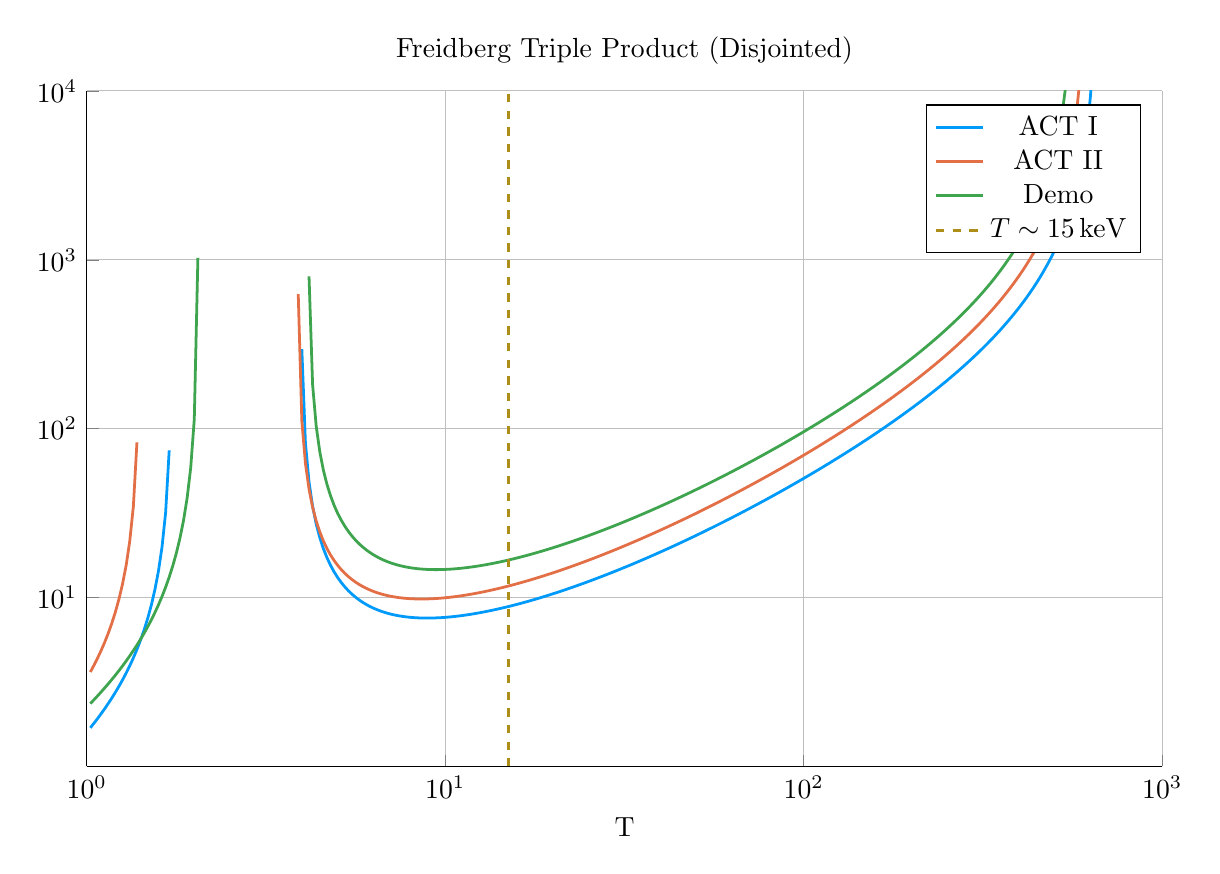
\begin{tikzpicture}[]
\begin{axis}[height = {101.6mm}, ylabel = {}, title = {Freidberg Triple Product (Disjointed)}, xmin = {1.0}, xmax = {1000.0}, ymax = {10000.0}, ymode = {log}, xlabel = {T}, {unbounded coords=jump, xticklabel style={rotate = 0}, log basis x=10, xmajorgrids = true, xtick = {1.0,10.0,100.0,1000.0}, xticklabels = {$10^{0}$,$10^{1}$,$10^{2}$,$10^{3}$}, xtick align = inside, axis lines* = left, yticklabel style={rotate = 0}, log basis y=10, ymajorgrids = true, ytick = {10.0,100.0,1000.0,10000.0}, yticklabels = {$10^{1}$,$10^{2}$,$10^{3}$,$10^{4}$}, ytick align = inside, axis lines* = left,     xshift = 0.0mm,
    yshift = 0.0mm,
    axis background/.style={fill={rgb,1:red,1.00000000;green,1.00000000;blue,1.00000000}}
}, xmode = {log}, ymin = {1.001}, width = {152.4mm}]\addplot+ [color = {rgb,1:red,0.00000000;green,0.60560316;blue,0.97868012},
draw opacity=1.0,
line width=1,
solid,mark = none,
mark size = 2.0,
mark options = {
    color = {rgb,1:red,0.00000000;green,0.00000000;blue,0.00000000}, draw opacity = 1.0,
    fill = {rgb,1:red,0.00000000;green,0.60560316;blue,0.97868012}, fill opacity = 1.0,
    line width = 1,
    rotate = 0,
    solid
}]coordinates {
(1.023292992280754, 1.6945150918881617)
(1.0471285480508996, 1.8022297212985727)
(1.0715193052376064, 1.9208400907418741)
(1.096478196143185, 2.0520379173824526)
(1.1220184543019633, 2.1978809957158)
(1.1481536214968828, 2.3608969492317664)
(1.1748975549395295, 2.5442241968703065)
(1.202264434617413, 2.7518066614453685)
(1.2302687708123816, 2.9886676965649497)
(1.2589254117941673, 3.2613035039971368)
(1.288249551693134, 3.5782615298822504)
(1.318256738556407, 3.9510138131485064)
(1.3489628825916535, 4.395316889582276)
(1.3803842646028848, 4.933406616196546)
(1.4125375446227544, 5.597693756447026)
(1.4454397707459274, 6.437310966298612)
(1.4791083881682074, 7.530455822814955)
(1.5135612484362082, 9.009551106277522)
(1.5488166189124815, 11.117997739838028)
(1.5848931924611136, 14.357045698731298)
(1.62181009735893, 19.94980446331863)
(1.6595869074375607, 31.870474474777332)
(1.6982436524617444, 74.50886497100848)
(1.7378008287493754, -268.62399052136783)
(1.7782794100389228, -49.919103932965776)
(1.8197008586099834, -28.182974323791697)
(1.8620871366628675, -19.98239680052841)
(1.9054607179632472, -15.70205772252279)
(1.9498445997580451, -13.093397062325929)
(1.9952623149688795, -11.354078520088276)
(2.041737944669529, -10.126703775296521)
(2.0892961308540396, -9.228291825900367)
(2.137962089502232, -8.555793230466092)
(2.1877616239495525, -8.047086394966504)
(2.2387211385683394, -7.662850026356773)
(2.290867652767773, -7.377360182440818)
(2.344228815319922, -7.173493942563709)
(2.3988329190194904, -7.03987823872135)
(2.4547089156850306, -6.969209177348767)
(2.51188643150958, -6.957252425128463)
(2.5703957827688635, -7.0022689551713535)
(2.6302679918953817, -7.104731798631218)
(2.6915348039269156, -7.2672686328905565)
(2.7542287033381663, -7.494810686078433)
(2.8183829312644537, -7.794966372176634)
(2.884031503126606, -8.178679918245468)
(2.9512092266663856, -8.661293939987127)
(3.019951720402016, -9.264230780294357)
(3.0902954325135905, -10.01767902164183)
(3.1622776601683795, -10.964999922356022)
(3.2359365692962827, -12.170236892008582)
(3.311311214825911, -13.7315665677587)
(3.3884415613920256, -15.806961575136446)
(3.4673685045253166, -18.667256898848134)
(3.548133892335755, -22.818098057023896)
(3.630780547701014, -29.323816090272153)
(3.715352290971725, -40.87190947609052)
(3.8018939632056115, -66.7704951710188)
(3.890451449942806, -176.00214091027135)
(3.9810717055349722, 296.2120048547568)
(4.073802778041127, 82.22608375442015)
(4.168693834703354, 48.43306336833725)
(4.265795188015927, 34.70962566295797)
(4.36515832240166, 27.295945016455207)
(4.466835921509632, 22.67019834453781)
(4.570881896148751, 19.52007287600256)
(4.677351412871983, 17.24499928723126)
(4.786300923226384, 15.531278040885976)
(4.897788193684462, 14.199095003080004)
(5.011872336272722, 13.138001469719821)
(5.1286138399136485, 12.27642393656205)
(5.248074602497725, 11.565956055783074)
(5.370317963702527, 10.972696881733755)
(5.495408738576246, 10.472204393849793)
(5.623413251903491, 10.04641840843593)
(5.7543993733715695, 9.681711040383625)
(5.88843655355589, 9.367610463946743)
(6.025595860743578, 9.095941481219963)
(6.165950018614822, 8.860232308719008)
(6.309573444801933, 8.655296117741381)
(6.456542290346556, 8.476930095683173)
(6.606934480075959, 8.321695258418004)
(6.760829753919817, 8.186752828259676)
(6.918309709189364, 8.06974093001644)
(7.079457843841379, 7.968680480243153)
(7.244359600749901, 7.881902520894599)
(7.413102413009175, 7.80799150193639)
(7.5857757502918375, 7.745740605469891)
(7.762471166286917, 7.694116194091195)
(7.943282347242816, 7.652229324407223)
(8.128305161640993, 7.619312722352829)
(8.31763771102671, 7.594702046961867)
(8.511380382023766, 7.577820541204338)
(8.709635899560805, 7.568166379774354)
(8.912509381337454, 7.565302179476453)
(9.120108393559097, 7.568846255848602)
(9.33254300796991, 7.57846529863635)
(9.549925860214358, 7.593868207120024)
(9.772372209558107, 7.614800878969009)
(10.0, 7.6410417872330525)
(10.232929922807541, 7.672398212107776)
(10.471285480508996, 7.708703019333509)
(10.715193052376065, 7.7498118970722105)
(10.964781961431852, 7.7956009790373795)
(11.220184543019636, 7.845964794420564)
(11.481536214968829, 7.9008144954472845)
(11.748975549395297, 7.960076321728849)
(12.02264434617413, 8.023690267358889)
(12.302687708123818, 8.091608922249174)
(12.589254117941675, 8.163796463753897)
(12.882495516931343, 8.240227778388245)
(13.182567385564074, 8.320887696558643)
(13.489628825916533, 8.405770325808698)
(13.803842646028846, 8.494878470244457)
(14.12537544622754, 8.588223125611163)
(14.454397707459272, 8.68582304101473)
(14.791083881682072, 8.787704339563915)
(15.13561248436208, 8.893900191356126)
(15.488166189124811, 9.00445053273945)
(15.848931924611133, 9.119401827772037)
(16.218100973589298, 9.238806866525163)
(16.595869074375607, 9.36272459734332)
(16.982436524617444, 9.49121998943775)
(17.378008287493753, 9.62436392387273)
(17.78279410038923, 9.762233108678469)
(18.197008586099834, 9.904910018476908)
(18.620871366628677, 10.052482855035347)
(19.054607179632473, 10.205045527912834)
(19.498445997580454, 10.362697653760055)
(19.952623149688797, 10.525544573138253)
(20.417379446695296, 10.693697383890798)
(20.892961308540396, 10.86727299025056)
(21.379620895022324, 11.04639416699954)
(21.87761623949553, 11.231189638117145)
(22.3872113856834, 11.42179416946176)
(22.908676527677734, 11.6183486751283)
(23.442288153199225, 11.82100033721453)
(23.9883291901949, 12.029902739089)
(24.547089156850298, 12.245216010109123)
(25.118864315095795, 12.467106987583263)
(25.703957827688633, 12.695749386290691)
(26.302679918953814, 12.931323985371597)
(26.915348039269155, 13.174018826913404)
(27.542287033381662, 13.424029428392666)
(28.183829312644534, 13.681559008968577)
(28.84031503126606, 13.946818729958853)
(29.512092266663856, 14.220027949885045)
(30.19951720402016, 14.50141449453101)
(30.902954325135905, 14.791214942515055)
(31.622776601683793, 15.089674926934103)
(32.359365692962825, 15.39704945369735)
(33.11311214825911, 15.713603237227478)
(33.884415613920254, 16.039611054270374)
(34.673685045253166, 16.375358304735574)
(35.48133892335755, 16.72114046362978)
(36.30780547701014, 17.077265375464844)
(37.15352290971726, 17.444051808101882)
(38.018939632056124, 17.821830851190978)
(38.90451449942807, 18.210946209955225)
(39.810717055349734, 18.611754712404426)
(40.73802778041128, 19.02462684323082)
(41.68693834703355, 19.44994730585631)
(42.65795188015925, 19.888115614110824)
(43.65158322401658, 20.33954671581207)
(44.6683592150963, 20.804671648648)
(45.708818961487495, 21.283938232164516)
(46.77351412871981, 21.777811796588267)
(47.86300923226383, 22.286775951266307)
(48.97788193684461, 22.811333395047512)
(50.11872336272722, 23.352006771196773)
(51.28613839913648, 23.90933956979331)
(52.48074602497726, 24.483897079598876)
(53.70317963702527, 25.07626739512277)
(54.954087385762456, 25.687062479009892)
(56.23413251903491, 26.316919285823328)
(57.543993733715695, 26.966500951119475)
(58.8843655355589, 27.63649804806381)
(60.25595860743578, 28.32762991928082)
(61.65950018614822, 29.040646086657393)
(63.09573444801933, 29.776327745458484)
(64.56542290346556, 30.535489348458338)
(66.06934480075961, 31.318980286421752)
(67.60829753919819, 32.12768667178653)
(69.18309709189366, 32.96253323296315)
(70.79457843841381, 33.82448532728458)
(72.44359600749902, 34.71455108131369)
(74.13102413009177, 35.63378366795554)
(75.85775750291836, 36.5832837306308)
(77.62471166286916, 37.56420196565578)
(79.43282347242814, 38.5777418749493)
(81.2830516164099, 39.625162702259914)
(83.17637711026708, 40.70778256728596)
(85.11380382023764, 41.82698181336084)
(87.09635899560806, 42.98420658580859)
(89.12509381337455, 44.18097265965641)
(91.20108393559097, 45.41886953713795)
(93.3254300796991, 46.69956483735465)
(95.49925860214358, 48.0248090026031)
(97.72372209558107, 49.39644034825024)
(100.0, 50.81639048567384)
(102.32929922807536, 52.28669015071427)
(104.71285480508996, 53.809475473344484)
(107.1519305237606, 55.38699472789598)
(109.64781961431851, 57.02161560723521)
(112.2018454301963, 58.71583306880927)
(114.81536214968828, 60.47227780555281)
(117.48975549395291, 62.29372540032026)
(120.22644346174131, 64.1831062288853)
(123.02687708123811, 66.14351618370313)
(125.89254117941675, 68.17822829869775)
(128.82495516931337, 70.29070536425795)
(131.82567385564073, 72.48461363302665)
(134.89628825916532, 74.76383772515437)
(138.03842646028852, 77.13249686084183)
(141.2537544622754, 79.59496255677749)
(144.5439770745928, 82.1558779437945)
(147.91083881682073, 84.82017888112068)
(151.35612484362088, 87.59311706484252)
(154.88166189124811, 90.48028535342075)
(158.48931924611142, 93.48764556200553)
(162.18100973589299, 96.62155901048361)
(165.95869074375614, 99.88882014839527)
(169.82436524617444, 103.29669362390514)
(173.78008287493762, 106.8529552149526)
(177.82794100389228, 110.56593709971621)
(181.97008586099827, 114.44457801209604)
(186.20871366628674, 118.49847890775631)
(190.54607179632464, 122.73796485951151)
(194.98445997580455, 127.17415401000369)
(199.52623149688787, 131.81903453779776)
(204.17379446695296, 136.68555074397534)
(208.92961308540387, 141.7876995445982)
(213.79620895022325, 147.14063886569335)
(218.77616239495518, 152.76080968855555)
(223.872113856834, 158.66607379276888)
(229.08676527677724, 164.87586960296383)
(234.42288153199226, 171.4113889762298)
(239.88329190194898, 178.29577828677515)
(245.4708915685031, 185.55436779375145)
(251.18864315095797, 193.21493404336246)
(257.03957827688646, 201.30800099096868)
(263.02679918953817, 209.86718667547356)
(269.1534803926917, 218.92960369175984)
(275.4228703338166, 228.5363234580894)
(281.8382931264455, 238.73291645637224)
(288.40315031266056, 249.57008335444863)
(295.1209226666387, 261.10439535985074)
(301.9951720402016, 273.39916651425244)
(309.0295432513592, 286.52548620009975)
(316.22776601683796, 300.5634472677593)
(323.5936569296281, 315.60361443723326)
(331.1311214825911, 331.74878965791873)
(338.84415613920237, 349.11614693461144)
(346.73685045253166, 367.83983008944125)
(354.8133892335753, 388.074134968045)
(363.0780547701014, 409.9974354672692)
(371.5352290971724, 433.8170644462405)
(380.1893963205613, 459.775431919879)
(389.04514499428046, 488.15776259296996)
(398.1071705534973, 519.301975844092)
(407.3802778041126, 553.6114337377378)
(416.8693834703355, 591.5715777555781)
(426.57951880159254, 633.7719123174471)
(436.5158322401661, 680.9354532594568)
(446.683592150963, 733.9587765720896)
(457.0881896148752, 793.9674013286159)
(467.73514128719813, 862.3938269620526)
(478.6300923226385, 941.0898231518593)
(489.77881936844614, 1032.4918995815904)
(501.18723362727246, 1139.8718558647272)
(512.8613839913648, 1267.728232380304)
(524.8074602497728, 1422.4206670383826)
(537.0317963702527, 1613.2432940240717)
(549.5408738576248, 1854.3379168248518)
(562.341325190349, 2168.328384373693)
(575.4399373371566, 2593.8014145005036)
(588.843655355589, 3202.400412559708)
(602.5595860743575, 4143.871725688599)
(616.5950018614822, 5792.368998792458)
(630.957344480193, 9418.65571693456)
(645.6542290346556, 23889.28171950775)
(660.6934480075957, -49140.70577934398)
(676.0829753919819, -12421.08556602776)
(691.8309709189363, -7211.5383604203)
(707.945784384138, -5131.503513512916)
(724.4359600749899, -4013.149779314024)
(741.3102413009177, -3315.290437938855)
(758.5775750291835, -2838.6775691444445)
(776.247116628692, -2492.7815835486012)
(794.3282347242813, -2230.5404344031062)
(812.8305161640995, -2025.0671265994276)
(831.7637711026708, -1859.8852065397507)
(851.1380382023768, -1724.3348515292655)
(870.9635899560806, -1611.214292586841)
(891.2509381337459, -1515.482798133364)
(912.0108393559096, -1433.5066904171208)
(933.2543007969915, -1362.60044755666)
(954.992586021436, -1300.7364064371823)
(977.2372209558112, -1246.3549673169614)
(1000.0, -1198.236922422159)
(1023.2929922807537, -1155.4154111586524)
(1047.1285480508996, -1117.1138595692732)
(1071.519305237606, -1082.7013755947412)
(1096.4781961431852, -1051.6601296512954)
(1122.018454301963, -1023.5611236164838)
(1148.1536214968828, -998.0459352192751)
(1174.897554939529, -974.8127865165062)
(1202.2644346174131, -953.6057869052796)
(1230.268770812381, -934.2065376059747)
(1258.9254117941675, -916.427514142416)
(1288.2495516931335, -900.1068024887031)
(1318.2567385564075, -885.1038764728944)
(1348.9628825916532, -871.2961837984906)
(1380.3842646028852, -858.5763656093441)
(1412.537544622754, -846.8499765447623)
(1445.439770745928, -836.0336032365552)
(1479.1083881682073, -826.0533023067777)
(1513.5612484362086, -816.8432963076928)
(1548.816618912481, -808.3448792375339)
(1584.893192461114, -800.5054933601936)
(1621.8100973589299, -793.2779468416144)
(1659.5869074375614, -786.619747763086)
(1698.2436524617442, -780.4925348022881)
(1737.8008287493763, -774.8615885976767)
(1778.2794100389228, -769.695410762998)
(1819.7008586099826, -764.9653598706944)
(1862.0871366628676, -760.6453356042871)
(1905.4607179632462, -756.7115038241651)
(1949.8445997580454, -753.1420564513764)
(1995.2623149688789, -749.9170011631115)
(2041.7379446695295, -747.017976692142)
(2089.296130854039, -744.4280901019075)
(2137.9620895022326, -742.1317730997671)
(2187.761623949552, -740.1146548191589)
(2238.72113856834, -738.3634489135239)
(2290.8676527677726, -736.8658531085748)
(2344.228815319923, -735.6104596965912)
(2398.83291901949, -734.5866754712753)
(2454.708915685031, -733.7846501343085)
(2511.88643150958, -733.1952120249796)
(2570.3957827688646, -732.8098103606878)
(2630.2679918953813, -732.6204632251878)
(2691.5348039269165, -732.619710649065)
(2754.2287033381663, -732.8005722110505)
(2818.382931264455, -733.1565086609373)
(2884.031503126606, -733.6813871269079)
(2951.209226666387, -734.3694495236135)
(3019.9517204020162, -735.2152838235631)
(3090.295432513592, -736.2137978944917)
(3162.2776601683795, -737.3601956401093)
(3235.936569296281, -738.6499552119711)
(3311.311214825911, -740.0788090865385)
(3388.441561392024, -741.6427258246325)
(3467.368504525317, -743.3378933506358)
(3548.133892335753, -745.1607036065371)
(3630.780547701014, -747.1077384514889)
(3715.352290971724, -749.1757566912511)
(3801.8939632056126, -751.3616821340012)
(3890.4514499428046, -753.6625925796814)
(3981.0717055349733, -756.0757096595084)
(4073.802778041126, -758.5983894506668)
(4168.693834703355, -761.2281137986595)
(4265.795188015925, -763.9624822864063)
(4365.158322401661, -766.7992045807192)
(4466.835921509631, -769.7360946070586)
(4570.881896148751, -772.7710620056145)
(4677.351412871981, -775.9021083311076)
(4786.300923226385, -779.1273204560445)
(4897.7881936844615, -782.4448656456962)
(5011.872336272725, -785.8529867735253)
(5128.613839913648, -789.3499978635558)
(5248.074602497728, -792.9342799342446)
(5370.317963702527, -796.604277116354)
(5495.408738576249, -800.3584930490041)
(5623.413251903491, -804.195487472099)
(5754.399373371566, -808.1138730792338)
(5888.43655355589, -812.1123125544108)
(6025.595860743575, -816.1895158014244)
(6165.9500186148225, -820.3442373483241)
(6309.57344480193, -824.575273914367)
(6456.542290346556, -828.8814621278906)
(6606.934480075957, -833.2616763844619)
(6760.829753919818, -837.7148268354883)
(6918.309709189362, -842.2398574982564)
(7079.457843841381, -846.8357444790493)
(7244.359600749898, -851.5014943016532)
(7413.102413009177, -856.2361423341288)
(7585.775750291836, -861.0387513072818)
(7762.4711662869195, -865.9084099187404)
(7943.282347242814, -870.8442315170112)
(8128.305161640995, -875.8453528602984)
(8317.63771102671, -880.9109329452398)
(8511.380382023768, -886.0401519010943)
(8709.635899560806, -891.2322099451943)
(8912.509381337459, -896.4863263958177)
(9120.108393559096, -901.8017387388758)
(9332.543007969914, -907.1777017450888)
(9549.92586021436, -912.6134865547074)
(9772.372209558112, -918.1083801920363)
(10000.0, -923.6616844862497)
};
\addlegendentry{ACT I}
\addplot+ [color = {rgb,1:red,0.88887350;green,0.43564919;blue,0.27812294},
draw opacity=1.0,
line width=1,
solid,mark = none,
mark size = 2.0,
mark options = {
    color = {rgb,1:red,0.00000000;green,0.00000000;blue,0.00000000}, draw opacity = 1.0,
    fill = {rgb,1:red,0.88887350;green,0.43564919;blue,0.27812294}, fill opacity = 1.0,
    line width = 1,
    rotate = 0,
    solid
}]coordinates {
(1.023292992280754, 3.6262198595749764)
(1.0471285480508996, 3.9709951177889846)
(1.0715193052376064, 4.3756174014389835)
(1.096478196143185, 4.856923072933348)
(1.1220184543019633, 5.438683072221177)
(1.1481536214968828, 6.155573870975628)
(1.1748975549395295, 7.060228008162098)
(1.202264434617413, 8.236563724204407)
(1.2302687708123816, 9.827054231195484)
(1.2589254117941673, 12.094532497587037)
(1.288249551693134, 15.583209353705142)
(1.318256738556407, 21.63257843385939)
(1.3489628825916535, 34.66570824747554)
(1.3803842646028848, 83.08790958003418)
(1.4125375446227544, -237.94957827646257)
(1.4454397707459274, -50.355280711590225)
(1.4791083881682074, -28.63496801892399)
(1.5135612484362082, -20.251666213285585)
(1.5488166189124815, -15.820177297479631)
(1.5848931924611136, -13.08951908492532)
(1.62181009735893, -11.24674808778935)
(1.6595869074375607, -9.926910662341783)
(1.6982436524617444, -8.941965953571943)
(1.7378008287493754, -8.185314268502955)
(1.7782794100389228, -7.592149139482488)
(1.8197008586099834, -7.120936958963385)
(1.8620871366628675, -6.74396430844709)
(1.9054607179632472, -6.442168044456181)
(1.9498445997580451, -6.202147460832283)
(1.9952623149688795, -6.014359309768401)
(2.041737944669529, -5.871988456076733)
(2.0892961308540396, -5.770222564971642)
(2.137962089502232, -5.705778915745288)
(2.1877616239495525, -5.676595450141278)
(2.2387211385683394, -5.68163408082953)
(2.290867652767773, -5.720765456471678)
(2.344228815319922, -5.794717627708497)
(2.3988329190194904, -5.9050800796980125)
(2.4547089156850306, -6.054361567255678)
(2.51188643150958, -6.246106580679075)
(2.5703957827688635, -6.485082333271136)
(2.6302679918953817, -6.777557290905968)
(2.6915348039269156, -7.1317054161224025)
(2.7542287033381663, -7.558190626573394)
(2.8183829312644537, -8.071018969252556)
(2.884031503126606, -8.688801804272321)
(2.9512092266663856, -9.436671353402025)
(3.019951720402016, -10.349269580424053)
(3.0902954325135905, -11.475575910838932)
(3.1622776601683795, -12.887036452859418)
(3.2359365692962827, -14.691959839828085)
(3.311311214825911, -17.06263857450721)
(3.3884415613920256, -20.29057894681975)
(3.4673685045253166, -24.910913722214016)
(3.548133892335755, -32.02376727816436)
(3.630780547701014, -44.30667919768318)
(3.715352290971725, -70.4202182892387)
(3.8018939632056115, -162.8647166076088)
(3.890451449942806, 626.9103884763274)
(3.9810717055349722, 111.1855857788192)
(4.073802778041127, 62.30641416623654)
(4.168693834703354, 43.93800066040291)
(4.265795188015927, 34.33706014393487)
(4.36515832240166, 28.454603024787982)
(4.466835921509632, 24.493996588522855)
(4.570881896148751, 21.655444964297164)
(4.677351412871983, 19.528883534080794)
(4.786300923226384, 17.882391475312325)
(4.897788193684462, 16.574948455957568)
(5.011872336272722, 15.51588818674524)
(5.1286138399136485, 14.644277005698534)
(5.248074602497725, 13.917659005030185)
(5.370317963702527, 13.305553561598769)
(5.495408738576246, 12.785518065105022)
(5.623413251903491, 12.340668088629867)
(5.7543993733715695, 11.958062188819154)
(5.88843655355589, 11.627618960477479)
(6.025595860743578, 11.341372389870859)
(6.165950018614822, 11.092948328333481)
(6.309573444801933, 10.877189105947096)
(6.456542290346556, 10.689879592932128)
(6.606934480075959, 10.527544110660646)
(6.760829753919817, 10.387293705403508)
(6.918309709189364, 10.266709799369176)
(7.079457843841379, 10.16375450253595)
(7.244359600749901, 10.076700725700801)
(7.413102413009175, 10.004077180609906)
(7.5857757502918375, 9.944624699045534)
(7.762471166286917, 9.897261247744884)
(7.943282347242816, 9.861053688507223)
(8.128305161640993, 9.835194817415095)
(8.31763771102671, 9.818984570337387)
(8.511380382023766, 9.811814542185662)
(8.709635899560805, 9.813155162447515)
(8.912509381337454, 9.822545006156611)
(9.120108393559097, 9.83958185650335)
(9.33254300796991, 9.863915174108707)
(9.549925860214358, 9.895239747025146)
(9.772372209558107, 9.933290289132369)
(10.0, 9.977836853773296)
(10.232929922807541, 10.028680908432321)
(10.471285480508996, 10.085651971057402)
(10.715193052376065, 10.148604718433416)
(10.964781961431852, 10.21741649362127)
(11.220184543019636, 10.291985152574611)
(11.481536214968829, 10.37222719997026)
(11.748975549395297, 10.458076172688434)
(12.02264434617413, 10.549481236152369)
(12.302687708123818, 10.64640596430817)
(12.589254117941675, 10.748827278619041)
(12.882495516931343, 10.856734525250282)
(13.182567385564074, 10.970128672782435)
(13.489628825916533, 11.089021615426763)
(13.803842646028846, 11.213435568926192)
(14.12537544622754, 11.343402548181452)
(14.454397707459272, 11.478963917208173)
(14.791083881682072, 11.620170003356527)
(15.13561248436208, 11.767079768850763)
(15.488166189124811, 11.919760533665668)
(15.848931924611133, 12.078287744603548)
(16.218100973589298, 12.242744785962834)
(16.595869074375607, 12.413222828300148)
(16.982436524617444, 12.589820711506782)
(17.378008287493753, 12.772644859640952)
(17.78279410038923, 12.961809224911852)
(18.197008586099834, 13.157435258695006)
(18.620871366628677, 13.359651907740494)
(19.054607179632473, 13.568595633881658)
(19.498445997580454, 13.78441045660099)
(19.952623149688797, 14.007248015617566)
(20.417379446695296, 14.237267654769363)
(20.892961308540396, 14.474636524779191)
(21.379620895022324, 14.719529704908814)
(21.87761623949553, 14.972130342899538)
(22.3872113856834, 15.232629812825081)
(22.908676527677734, 15.501227890845222)
(23.442288153199225, 15.778132947219865)
(23.9883291901949, 16.06356215819839)
(24.547089156850298, 16.35774173268541)
(25.118864315095795, 16.660907159108888)
(25.703957827688633, 16.973303467018464)
(26.302679918953814, 17.295185509573656)
(26.915348039269155, 17.62681826308181)
(27.542287033381662, 17.96847714569595)
(28.183829312644534, 18.32044835551375)
(28.84031503126606, 18.6830292286709)
(29.512092266663856, 19.05652861809976)
(30.19951720402016, 19.441267293702094)
(30.902954325135905, 19.837578364764788)
(31.622776601683793, 20.245807725529637)
(32.359365692962825, 20.66631452491334)
(33.11311214825911, 21.099471661462132)
(33.884415613920254, 21.54566630471813)
(34.673685045253166, 22.00530044427105)
(35.48133892335755, 22.47879146787113)
(36.30780547701014, 22.966572770086653)
(37.15352290971726, 23.469094393103948)
(38.018939632056124, 23.986823701388534)
(38.90451449942807, 24.520246092055554)
(39.810717055349734, 25.069865742935068)
(40.73802778041128, 25.636206400465333)
(41.68693834703355, 26.219812206925383)
(42.65795188015925, 26.82124858892035)
(43.65158322401658, 27.441103151399624)
(44.6683592150963, 28.079986677312778)
(45.708818961487495, 28.73853413868146)
(46.77351412871981, 29.417405780721598)
(47.86300923226383, 30.117288263079946)
(48.97788193684461, 30.838895864745762)
(50.11872336272722, 31.582971756705206)
(51.28613839913648, 32.35028934671438)
(52.48074602497726, 33.14165370090234)
(53.70317963702527, 33.957903047277725)
(54.954087385762456, 34.79991036660676)
(56.23413251903491, 35.668585076557704)
(57.543993733715695, 36.56487481530732)
(58.8843655355589, 37.4897673324607)
(60.25595860743578, 38.44429249224886)
(61.65950018614822, 39.42952440027207)
(63.09573444801933, 40.44658366003865)
(64.56542290346556, 41.496639769647544)
(66.06934480075961, 42.58091366862388)
(67.60829753919819, 43.70068044592992)
(69.18309709189366, 44.857272221109575)
(70.79457843841381, 46.052081211550274)
(72.44359600749902, 47.286562999969696)
(74.13102413009177, 48.562240017471)
(75.85775750291836, 49.8807052588659)
(77.62471166286916, 51.243626248459464)
(79.43282347242814, 52.65274927613318)
(81.2830516164099, 54.10990392537751)
(83.17637711026708, 55.617007916924386)
(85.11380382023764, 57.17607229384146)
(87.09635899560806, 58.78920697639489)
(89.12509381337455, 60.458626717694976)
(91.20108393559097, 62.18665749414143)
(93.3254300796991, 63.97574336801635)
(95.49925860214358, 65.82845386036456)
(97.72372209558107, 67.74749189972668)
(100.0, 69.73570233531223)
(102.32929922807536, 71.79608117146411)
(104.71285480508996, 73.93178548206338)
(107.1519305237606, 76.14614413306579)
(109.64781961431851, 78.44266936696852)
(112.2018454301963, 80.8250693343548)
(114.81536214968828, 83.29726166380183)
(117.48975549395291, 85.86338817160895)
(120.22644346174131, 88.52783082428154)
(123.02687708123811, 91.29522907965378)
(125.89254117941675, 94.17049874718609)
(128.82495516931337, 97.15885252455993)
(131.82567385564073, 100.26582238652995)
(134.89628825916532, 103.497284023392)
(138.03842646028852, 106.8594835506073)
(141.2537544622754, 110.35906674040386)
(144.5439770745928, 114.00311105358536)
(147.91083881682073, 117.79916079358593)
(151.35612484362088, 121.75526573929804)
(154.88166189124811, 125.88002366576029)
(158.48931924611142, 130.1826272158626)
(162.18100973589299, 134.672915650604)
(165.95869074375614, 139.36143207981326)
(169.82436524617444, 144.25948686159074)
(173.78008287493762, 149.37922795930874)
(177.82794100389228, 154.73371916238966)
(181.97008586099827, 160.33702721452812)
(186.20871366628674, 166.20431905434293)
(190.54607179632464, 172.35197056339555)
(194.98445997580455, 178.79768844082054)
(199.52623149688787, 185.56064708952624)
(204.17379446695296, 192.66164271474446)
(208.92961308540387, 200.12326721230153)
(213.79620895022325, 207.97010486869286)
(218.77616239495518, 216.2289554844475)
(223.872113856834, 224.92908801677567)
(229.08676527677724, 234.10252996410594)
(234.42288153199226, 243.78439825504503)
(239.88329190194898, 254.013278913416)
(245.4708915685031, 264.831664041007)
(251.18864315095797, 276.2864564799751)
(257.03957827688646, 288.42955470570877)
(263.02679918953817, 301.31853323333485)
(269.1534803926917, 315.01743724146417)
(275.4228703338166, 329.5977144230688)
(281.8382931264455, 345.13931252826)
(288.40315031266056, 361.7319780177609)
(295.1209226666387, 379.47680017147866)
(301.9951720402016, 398.48805653482157)
(309.0295432513592, 418.8954306148157)
(316.22776601683796, 440.8466924729332)
(323.5936569296281, 464.5109589979699)
(331.1311214825911, 490.0826855730525)
(338.84415613920237, 517.7865879974996)
(346.73685045253166, 547.8837577991267)
(354.8133892335753, 580.6793227491402)
(363.0780547701014, 616.5321281016747)
(371.5352290971724, 655.8670890363044)
(380.1893963205613, 699.1911156139116)
(389.04514499428046, 747.1138767235202)
(398.1071705534973, 800.3752099841976)
(407.3802778041126, 859.8817991675508)
(416.8693834703355, 926.7569931156614)
(426.57951880159254, 1002.409608394075)
(436.5158322401661, 1088.6307275063882)
(446.683592150963, 1187.7327493644536)
(457.0881896148752, 1302.7538970715893)
(467.73514128719813, 1437.7671929229414)
(478.6300923226385, 1598.3619531251416)
(489.77881936844614, 1792.4217156957561)
(501.18723362727246, 2031.435864125701)
(512.8613839913648, 2332.8272604727294)
(524.8074602497728, 2724.3501891507594)
(537.0317963702527, 3253.0808589923313)
(549.5408738576248, 4005.7745115556468)
(562.341325190349, 5161.830905458572)
(575.4399373371566, 7161.999955047848)
(588.843655355589, 11456.916643900393)
(602.5595860743575, 27278.085748054084)
(616.5950018614822, -81374.99567859212)
(630.957344480193, -16777.758330681536)
(645.6542290346556, -9494.611990167594)
(660.6934480075957, -6689.456467425088)
(676.0829753919819, -5204.544925417548)
(691.8309709189363, -4286.084695387924)
(707.945784384138, -3662.3824611701343)
(724.4359600749899, -3211.5569830118793)
(741.3102413009177, -2870.7907078330154)
(758.5775750291835, -2604.4181322887152)
(776.247116628692, -2390.6863963037536)
(794.3282347242813, -2215.5742233715514)
(812.8305161640995, -2069.6372672190055)
(831.7637711026708, -1946.2815219657975)
(851.1380382023768, -1840.7635003469652)
(870.9635899560806, -1749.5836745614658)
(891.2509381337459, -1670.1038187095141)
(912.0108393559096, -1600.2974165784447)
(933.2543007969915, -1538.5821079233035)
(954.992586021436, -1483.704347654581)
(977.2372209558112, -1434.6582328197553)
(1000.0, -1390.6272443725638)
(1023.2929922807537, -1350.9416958920935)
(1047.1285480508996, -1315.0471613093978)
(1071.519305237606, -1282.4807127947604)
(1096.4781961431852, -1252.8528041238237)
(1122.018454301963, -1225.8332942321483)
(1148.1536214968828, -1201.1405477147484)
(1174.897554939529, -1178.5328496873165)
(1202.2644346174131, -1157.8015815679175)
(1230.268770812381, -1138.765750110663)
(1258.9254117941675, -1121.267566697522)
(1288.2495516931335, -1105.1688489426283)
(1318.2567385564075, -1090.348071514546)
(1348.9628825916532, -1076.6979335079102)
(1380.3842646028852, -1064.1233398013928)
(1412.537544622754, -1052.539716470997)
(1445.439770745928, -1041.8715974920947)
(1479.1083881682073, -1032.0514330898977)
(1513.5612484362086, -1023.018580214714)
(1548.816618912481, -1014.7184434731793)
(1584.893192461114, -1007.1017409878611)
(1621.8100973589299, -1000.1238744907862)
(1659.5869074375614, -993.744386783934)
(1698.2436524617442, -987.9264927488415)
(1737.8008287493763, -982.636672530169)
(1778.2794100389228, -977.8443174854673)
(1819.7008586099826, -973.5214210860804)
(1862.0871366628676, -969.6423082497454)
(1905.4607179632462, -966.1833976443339)
(1949.8445997580454, -963.1229923714116)
(1995.2623149688789, -960.4410951549132)
(2041.7379446695295, -958.1192447533882)
(2089.296130854039, -956.1403708072178)
(2137.9620895022326, -954.4886644127564)
(2187.761623949552, -953.1494647041984)
(2238.72113856834, -952.1091527568241)
(2290.8676527677726, -951.3550628814313)
(2344.228815319923, -950.8753984451814)
(2398.83291901949, -950.6591580412987)
(2454.708915685031, -950.6960687224226)
(2511.88643150958, -950.976525783883)
(2570.3957827688646, -951.4915383610024)
(2630.2679918953813, -952.2326801933348)
(2691.5348039269165, -953.1920450178479)
(2754.2287033381663, -954.3622060364678)
(2818.382931264455, -955.7361791027337)
(2884.031503126606, -957.3073891869254)
(2951.209226666387, -959.0696398044653)
(3019.9517204020162, -961.0170851050241)
(3090.295432513592, -963.1442043574473)
(3162.2776601683795, -965.4457785953113)
(3235.936569296281, -967.9168692139419)
(3311.311214825911, -970.5527983325226)
(3388.441561392024, -973.3491307549663)
(3467.368504525317, -976.301657380888)
(3548.133892335753, -979.406379933558)
(3630.780547701014, -982.6594968855042)
(3715.352290971724, -986.0573904745661)
(3801.8939632056126, -989.5966147140405)
(3890.4514499428046, -993.2738843101055)
(3981.0717055349733, -997.0860644082568)
(4073.802778041126, -1001.030161098068)
(4168.693834703355, -1005.1033126123773)
(4265.795188015925, -1009.3027811630325)
(4365.158322401661, -1013.6259453607602)
(4466.835921509631, -1018.0702931715625)
(4570.881896148751, -1022.633415366397)
(4677.351412871981, -1027.3129994248159)
(4786.300923226385, -1032.1068237614704)
(4897.7881936844615, -1037.0127529096899)
(5011.872336272725, -1042.0287316317933)
(5128.613839913648, -1047.1527812631514)
(5248.074602497728, -1052.3829949308802)
(5370.317963702527, -1057.7175336249259)
(5495.408738576249, -1063.1546224338358)
(5623.413251903491, -1068.6925470213334)
(5754.399373371566, -1074.3296503261488)
(5888.43655355589, -1080.0643294689673)
(6025.595860743575, -1085.8950328516705)
(6165.9500186148225, -1091.8202574352306)
(6309.57344480193, -1097.8385461836895)
(6456.542290346556, -1103.9484856626516)
(6606.934480075957, -1110.1487037816134)
(6760.829753919818, -1116.437867667452)
(6918.309709189362, -1122.8146816767116)
(7079.457843841381, -1129.2778854970907)
(7244.359600749898, -1135.8262523843705)
(7413.102413009177, -1142.4585874877714)
(7585.775750291836, -1149.1737262727324)
(7762.4711662869195, -1155.9705330323777)
(7943.282347242814, -1162.847899481954)
(8128.305161640995, -1169.8047434309324)
(8317.63771102671, -1176.840007527851)
(8511.380382023768, -1183.9526580733384)
(8709.635899560806, -1191.141683897054)
(8912.509381337459, -1198.4060952946172)
(9120.108393559096, -1205.7449230208424)
(9332.543007969914, -1213.1572173358775)
(9549.92586021436, -1220.642047101055)
(9772.372209558112, -1228.198498921507)
(10000.0, -1235.8256763101228)
};
\addlegendentry{ACT II}
\addplot+ [color = {rgb,1:red,0.24222430;green,0.64327509;blue,0.30444865},
draw opacity=1.0,
line width=1,
solid,mark = none,
mark size = 2.0,
mark options = {
    color = {rgb,1:red,0.00000000;green,0.00000000;blue,0.00000000}, draw opacity = 1.0,
    fill = {rgb,1:red,0.24222430;green,0.64327509;blue,0.30444865}, fill opacity = 1.0,
    line width = 1,
    rotate = 0,
    solid
}]coordinates {
(1.023292992280754, 2.35717971253544)
(1.0471285480508996, 2.4818091803011884)
(1.0715193052376064, 2.6160533994079267)
(1.096478196143185, 2.7610169738489345)
(1.1220184543019633, 2.9179792560669826)
(1.1481536214968828, 3.088429876891961)
(1.1748975549395295, 3.2741132141278877)
(1.202264434617413, 3.4770845203202887)
(1.2302687708123816, 3.6997814161989337)
(1.2589254117941673, 3.9451158626625746)
(1.288249551693134, 4.216593759892962)
(1.318256738556407, 4.5184723163672)
(1.3489628825916535, 4.8559698120095405)
(1.3803842646028848, 5.235549216958988)
(1.4125375446227544, 5.6653077812466694)
(1.4454397707459274, 6.155521704098852)
(1.4791083881682074, 6.719422812007362)
(1.5135612484362082, 7.374331069416676)
(1.5488166189124815, 8.143348442005678)
(1.5848931924611136, 9.0579674025362)
(1.62181009735893, 10.162226448053275)
(1.6595869074375607, 11.51959922678817)
(1.6982436524617444, 13.224971744537322)
(1.7378008287493754, 15.426704428972686)
(1.7782794100389228, 18.37029833004982)
(1.8197008586099834, 22.493152913401733)
(1.8620871366628675, 28.65703826424774)
(1.9054607179632472, 38.826389394454985)
(1.9498445997580451, 58.65838956889421)
(1.9952623149688795, 113.86026736745272)
(2.041737944669529, 1028.465896265156)
(2.0892961308540396, -156.98955302050203)
(2.137962089502232, -75.58944517456705)
(2.1877616239495525, -51.04391619634808)
(2.2387211385683394, -39.30966054980392)
(2.290867652767773, -32.5119531577225)
(2.344228815319922, -28.143264194500333)
(2.3988329190194904, -25.158071654062468)
(2.4547089156850306, -23.0445846464956)
(2.51188643150958, -21.52440818514324)
(2.5703957827688635, -20.43488629677609)
(2.6302679918953817, -19.676536809340007)
(2.6915348039269156, -19.18724883626914)
(2.7542287033381663, -18.92875930297599)
(2.8183829312644537, -18.87930979578657)
(2.884031503126606, -19.02971234594769)
(2.9512092266663856, -19.381519932557275)
(3.019951720402016, -19.946725352708658)
(3.0902954325135905, -20.74884656063491)
(3.1622776601683795, -21.825612263340254)
(3.2359365692962827, -23.233892020991846)
(3.311311214825911, -25.05821583556076)
(3.3884415613920256, -27.425575246468597)
(3.4673685045253166, -30.532068258328167)
(3.548133892335755, -34.6936386598954)
(3.630780547701014, -40.450370735740485)
(3.715352290971725, -48.803893211628264)
(3.8018939632056115, -61.839107568518806)
(3.890451449942806, -84.72360389451674)
(3.9810717055349722, -134.73071514219606)
(4.073802778041127, -326.7218117310164)
(4.168693834703354, 798.2884776786321)
(4.265795188015927, 182.0559821932355)
(4.36515832240166, 103.75476422947621)
(4.466835921509632, 73.15084324411494)
(4.570881896148751, 56.90014770917698)
(4.677351412871983, 46.86280231089802)
(4.786300923226384, 40.07409117664327)
(4.897788193684462, 35.19587156238823)
(5.011872336272722, 31.53573209180628)
(5.1286138399136485, 28.69950502793406)
(5.248074602497725, 26.446359733467812)
(5.370317963702527, 24.620894487256926)
(5.495408738576246, 23.11837741508691)
(5.623413251903491, 21.86567883944471)
(5.7543993733715695, 20.81020944532067)
(5.88843655355589, 19.91319942113111)
(6.025595860743578, 19.145453338573617)
(6.165950018614822, 18.484578493662337)
(6.309573444801933, 17.91312275369926)
(6.456542290346556, 17.417291943801875)
(6.606934480075959, 16.98604667476511)
(6.760829753919817, 16.610453971230086)
(6.918309709189364, 16.283213587869994)
(7.079457843841379, 15.998306518944684)
(7.244359600749901, 15.750730470203408)
(7.413102413009175, 15.536298211082281)
(7.5857757502918375, 15.351482055139172)
(7.762471166286917, 15.193292627587141)
(7.943282347242816, 15.059183429252593)
(8.128305161640993, 14.946975025647662)
(8.31763771102671, 14.854794320700986)
(8.511380382023766, 14.781025536184384)
(8.709635899560805, 14.7242703555862)
(8.912509381337454, 14.683315302358887)
(9.120108393559097, 14.65710487318027)
(9.33254300796991, 14.644719282590849)
(9.549925860214358, 14.645355927794705)
(9.772372209558107, 14.658313873881836)
(10.0, 14.682980806167361)
(10.232929922807541, 14.718822009214483)
(10.471285480508996, 14.765371019745997)
(10.715193052376065, 14.822221669168664)
(10.964781961431852, 14.889021285358137)
(11.220184543019636, 14.965464866053368)
(11.481536214968829, 15.05129007022395)
(11.748975549395297, 15.14627290102121)
(12.02264434617413, 15.25022397586703)
(12.302687708123818, 15.362985297092992)
(12.589254117941675, 15.484427450328177)
(12.882495516931343, 15.614447171583684)
(13.182567385564074, 15.752965230502607)
(13.489628825916533, 15.899924588336324)
(13.803842646028846, 16.055288793998695)
(14.12537544622754, 16.219040587639775)
(14.454397707459272, 16.391180685479707)
(14.791083881682072, 16.571726724885952)
(15.13561248436208, 16.760712347737194)
(15.488166189124811, 16.95818640970398)
(15.848931924611133, 17.164212298589476)
(16.218100973589298, 17.378867350854325)
(16.595869074375607, 17.60224235578842)
(16.982436524617444, 17.834441138402067)
(17.378008287493753, 18.075580213329598)
(17.78279410038923, 18.325788503087594)
(18.197008586099834, 18.58520711493611)
(18.620871366628677, 18.85398917137603)
(19.054607179632473, 19.132299689997243)
(19.498445997580454, 19.420315508987848)
(19.952623149688797, 19.718225255134794)
(20.417379446695296, 20.026229351605068)
(20.892961308540396, 20.344540063200334)
(21.379620895022324, 20.673381577137132)
(21.87761623949553, 21.012990117724218)
(22.3872113856834, 21.36361409359547)
(22.908676527677734, 21.725514276034158)
(23.442288153199225, 22.09896400968359)
(23.9883291901949, 22.48424945066888)
(24.547089156850298, 22.881669834048008)
(25.118864315095795, 23.29153777529909)
(25.703957827688633, 23.714179595465023)
(26.302679918953814, 24.1499356783425)
(26.915348039269155, 24.599160856667968)
(27.542287033381662, 25.062224828200716)
(28.183829312644534, 25.539512602223876)
(28.84031503126606, 26.031424977123194)
(29.512092266663856, 26.53837904984218)
(30.19951720402016, 27.060808758149086)
(30.902954325135905, 27.599165456789784)
(31.622776601683793, 28.153918528740398)
(32.359365692962825, 28.725556028091596)
(33.11311214825911, 29.314585389840012)
(33.884415613920254, 29.92153410692588)
(34.673685045253166, 30.54695054518941)
(35.48133892335755, 31.191404729363835)
(36.30780547701014, 31.85548920357142)
(37.15352290971726, 32.539819934883965)
(38.018939632056124, 33.2450372671933)
(38.90451449942807, 33.97180692875365)
(39.810717055349734, 34.720821094770145)
(40.73802778041128, 35.49279951031094)
(41.68693834703355, 36.28849067540826)
(42.65795188015925, 37.10867309667045)
(43.65158322401658, 37.95415660928692)
(44.6683592150963, 38.82578377371943)
(45.708818961487495, 39.724431351691656)
(46.77351412871981, 40.65101186650543)
(47.86300923226383, 41.606475253047016)
(48.97788193684461, 42.59181060316595)
(50.11872336272722, 43.6080480128369)
(51.28613839913648, 44.65626053774646)
(52.48074602497726, 45.73756626505624)
(53.70317963702527, 46.8531305065716)
(54.954087385762456, 48.00416812806276)
(56.23413251903491, 49.191946015931904)
(57.543993733715695, 50.41778569686905)
(58.8843655355589, 51.68306611904523)
(60.25595860743578, 52.989226606822776)
(61.65950018614822, 54.33777000158897)
(63.09573444801933, 55.730266002386294)
(64.56542290346556, 57.16835472118021)
(66.06934480075961, 58.6537504688871)
(67.60829753919819, 60.188245789690065)
(69.18309709189366, 61.77371576271342)
(70.79457843841381, 63.41212259182487)
(72.44359600749902, 65.10552050177131)
(74.13102413009177, 66.85606099634911)
(75.85775750291836, 68.66599841255625)
(77.62471166286916, 70.53769595522424)
(79.43282347242814, 72.47363208934415)
(81.2830516164099, 74.47640741841091)
(83.17637711026708, 76.54875205648534)
(85.11380382023764, 78.69353354087694)
(87.09635899560806, 80.91376533210672)
(89.12509381337455, 83.21261595246393)
(91.20108393559097, 85.59341881965305)
(93.3254300796991, 88.05968283780572)
(95.49925860214358, 90.61510381458238)
(97.72372209558107, 93.26357678029993)
(100.0, 96.00920929309494)
(102.32929922807536, 98.85633582318225)
(104.71285480508996, 101.80953331943044)
(107.1519305237606, 104.87363807290143)
(109.64781961431851, 108.05376400487297)
(112.2018454301963, 111.35532252137295)
(114.81536214968828, 114.78404409266237)
(117.48975549395291, 118.34600173553473)
(120.22644346174131, 122.04763659144128)
(123.02687708123811, 125.89578583443561)
(125.89254117941675, 129.89771314265255)
(128.82495516931337, 134.06114202456072)
(131.82567385564073, 138.39429231126618)
(134.89628825916532, 142.9059201716157)
(138.03842646028852, 147.60536205264688)
(141.2537544622754, 152.50258300133495)
(144.5439770745928, 157.60822988511444)
(147.91083881682073, 162.93369009965753)
(151.35612484362088, 168.4911564345786)
(154.88166189124811, 174.29369885598337)
(158.48931924611142, 180.35534412396194)
(162.18100973589299, 186.6911641591149)
(165.95869074375614, 193.31737439360472)
(169.82436524617444, 200.25144347424498)
(173.78008287493762, 207.5122157275964)
(177.82794100389228, 215.12004829313008)
(181.97008586099827, 223.09696495296473)
(186.20871366628674, 231.46682908778078)
(190.54607179632464, 240.2555385901752)
(194.98445997580455, 249.49124605601838)
(199.52623149688787, 259.2046081609023)
(204.17379446695296, 269.42906883450684)
(208.92961308540387, 280.2011816981363)
(213.79620895022325, 291.56097826457074)
(218.77616239495518, 303.5523896585691)
(223.872113856834, 316.22373115690675)
(229.08676527677724, 329.6282607402076)
(234.42288153199226, 343.8248251873222)
(239.88329190194898, 358.87861014583916)
(245.4708915685031, 374.8620142351696)
(251.18864315095797, 391.8556717853743)
(257.03957827688646, 409.94965455513596)
(263.02679918953817, 429.2448900643584)
(269.1534803926917, 449.8548435069576)
(275.4228703338166, 471.90752218020964)
(281.8382931264455, 495.5478770458799)
(288.40315031266056, 520.9406962311275)
(295.1209226666387, 548.2741122773373)
(301.9951720402016, 577.7638805404314)
(309.0295432513592, 609.658634084495)
(316.22776601683796, 644.246385364096)
(323.5936569296281, 681.8626340181728)
(331.1311214825911, 722.90056349646)
(338.84415613920237, 767.8239827457569)
(346.73685045253166, 817.1839150307055)
(354.8133892335753, 871.6400930087617)
(363.0780547701014, 931.989139640923)
(371.5352290971724, 999.2019951154434)
(380.1893963205613, 1074.4743320439363)
(389.04514499428046, 1159.2955415953786)
(398.1071705534973, 1255.544792926278)
(407.3802778041126, 1365.6274291159207)
(416.8693834703355, 1492.6729473876055)
(426.57951880159254, 1640.8296437937745)
(436.5158322401661, 1815.7158629178796)
(446.683592150963, 2025.134400025375)
(457.0881896148752, 2280.2483682565407)
(467.73514128719813, 2597.6082486029304)
(478.6300923226385, 3002.8475902112687)
(489.77881936844614, 3537.9047470772252)
(501.18723362727246, 4276.437626628122)
(512.8613839913648, 5360.804039087363)
(524.8074602497728, 7106.509978464866)
(537.0317963702527, 10380.476417346483)
(549.5408738576248, 18740.455098272687)
(562.341325190349, 85036.83215617402)
(575.4399373371566, -35086.39752987788)
(588.843655355589, -14824.933467194654)
(602.5595860743575, -9511.977278291743)
(616.5950018614822, -7064.038279234583)
(630.957344480193, -5656.792430644577)
(645.6542290346556, -4743.611518297644)
(660.6934480075957, -4103.663600679462)
(676.0829753919819, -3630.666874390215)
(691.8309709189363, -3267.141624972824)
(707.945784384138, -2979.283771063334)
(724.4359600749899, -2745.9131518328722)
(741.3102413009177, -2553.0838928957774)
(758.5775750291835, -2391.238793241459)
(776.247116628692, -2253.6089391279506)
(794.3282347242813, -2135.266035761753)
(812.8305161640995, -2032.5366435303345)
(831.7637711026708, -1942.626727039276)
(851.1380382023768, -1863.373393859207)
(870.9635899560806, -1793.0762412000263)
(891.2509381337459, -1730.380039545634)
(912.0108393559096, -1674.1914023917016)
(933.2543007969915, -1623.6184845304515)
(954.992586021436, -1577.9266111000534)
(977.2372209558112, -1536.5051343507193)
(1000.0, -1498.8423376381347)
(1023.2929922807537, -1464.506195755428)
(1047.1285480508996, -1433.129456883747)
(1071.519305237606, -1404.3979545012546)
(1096.4781961431852, -1378.0413617663937)
(1122.018454301963, -1353.8258129276785)
(1148.1536214968828, -1331.5479662110808)
(1174.897554939529, -1311.030189991993)
(1202.2644346174131, -1292.116631877376)
(1230.268770812381, -1274.669987366889)
(1258.9254117941675, -1258.5688270146752)
(1288.2495516931335, -1243.7053726178099)
(1318.2567385564075, -1229.9836368136791)
(1348.9628825916532, -1217.317858631452)
(1380.3842646028852, -1205.6311814829392)
(1412.537544622754, -1194.8545308590062)
(1445.439770745928, -1184.925657395171)
(1479.1083881682073, -1175.7883175556403)
(1513.5612484362086, -1167.3915693829078)
(1548.816618912481, -1159.6891648877015)
(1584.893192461114, -1152.6390239508473)
(1621.8100973589299, -1146.202777256317)
(1659.5869074375614, -1140.3453679122392)
(1698.2436524617442, -1135.034703139298)
(1737.8008287493763, -1130.241348901597)
(1778.2794100389228, -1125.938261268496)
(1819.7008586099826, -1122.1005496540938)
(1862.0871366628676, -1118.7052674636907)
(1905.4607179632462, -1115.7312265701553)
(1949.8445997580454, -1113.158832506069)
(1995.2623149688789, -1110.9699377226104)
(2041.7379446695295, -1109.147710646497)
(2089.296130854039, -1107.6765185863496)
(2137.9620895022326, -1106.5418228099265)
(2187.761623949552, -1105.7300843423764)
(2238.72113856834, -1105.2286792298883)
(2290.8676527677726, -1105.0258221785482)
(2344.228815319923, -1105.110497619489)
(2398.83291901949, -1105.4723973724788)
(2454.708915685031, -1106.1018641839623)
(2511.88643150958, -1106.989840505089)
(2570.3957827688646, -1108.1278219524222)
(2630.2679918953813, -1109.5078149608594)
(2691.5348039269165, -1111.1222981961623)
(2754.2287033381663, -1112.964187344869)
(2818.382931264455, -1115.0268029431438)
(2884.031503126606, -1117.3038409443948)
(2951.209226666387, -1119.789345758937)
(3019.9517204020162, -1122.4776855282623)
(3090.295432513592, -1125.3635294222436)
(3162.2776601683795, -1128.4418267701806)
(3235.936569296281, -1131.707787856591)
(3311.311214825911, -1135.156866230195)
(3388.441561392024, -1138.7847423901355)
(3467.368504525317, -1142.5873087272637)
(3548.133892335753, -1146.560655610507)
(3630.780547701014, -1150.7010585192597)
(3715.352290971724, -1155.004966132348)
(3801.8939632056126, -1159.4689892927727)
(3890.4514499428046, -1164.089890775121)
(3981.0717055349733, -1168.8645757853008)
(4073.802778041126, -1173.7900831570503)
(4168.693834703355, -1178.863577129479)
(4265.795188015925, -1184.0823397373426)
(4365.158322401661, -1189.4437637081103)
(4466.835921509631, -1194.9453458488758)
(4570.881896148751, -1200.584680881554)
(4677.351412871981, -1206.359455692049)
(4786.300923226385, -1212.2674439620594)
(4897.7881936844615, -1218.306501154806)
(5011.872336272725, -1224.4745598284221)
(5128.613839913648, -1230.769625252875)
(5248.074602497728, -1237.189771308321)
(5370.317963702527, -1243.7331366445615)
(5495.408738576249, -1250.397921082915)
(5623.413251903491, -1257.1823822433182)
(5754.399373371566, -1264.0848323808139)
(5888.43655355589, -1271.1036354168307)
(6025.595860743575, -1278.237204151789)
(6165.9500186148225, -1285.4839976466099)
(6309.57344480193, -1292.8425187616258)
(6456.542290346556, -1300.311311778789)
(6606.934480075957, -1307.8889604695446)
(6760.829753919818, -1315.5740857720057)
(6918.309709189362, -1323.3653437726728)
(7079.457843841381, -1331.2614176554332)
(7244.359600749898, -1339.2610488818116)
(7413.102413009177, -1347.3629692622837)
(7585.775750291836, -1355.56596581618)
(7762.4711662869195, -1363.868846140099)
(7943.282347242814, -1372.2704436874026)
(8128.305161640995, -1380.7696164844647)
(8317.63771102671, -1389.36524591747)
(8511.380382023768, -1398.0562355854236)
(8709.635899560806, -1406.8415102153197)
(8912.509381337459, -1415.7200146357025)
(9120.108393559096, -1424.690712805097)
(9332.543007969914, -1433.7525868920366)
(9549.92586021436, -1442.904636402135)
(9772.372209558112, -1452.1458773584723)
(10000.0, -1461.475341509417)
};
\addlegendentry{Demo}
\addplot+ [color = {rgb,1:red,0.67554396;green,0.55566233;blue,0.09423434},
draw opacity=1.0,
line width=1,
dashed,mark = none,
mark size = 2.0,
mark options = {
    color = {rgb,1:red,0.00000000;green,0.00000000;blue,0.00000000}, draw opacity = 1.0,
    fill = {rgb,1:red,0.67554396;green,0.55566233;blue,0.09423434}, fill opacity = 1.0,
    line width = 1,
    rotate = 0,
    solid
}]coordinates {
(15.0, 1.0)
(15.0, 10000.0)
};
\addlegendentry{$T \sim 15 \, \textnormal{keV}$}
\end{axis}

\end{tikzpicture}

%		\end{adjustbox}
%        \caption{Reactors with Discontinuity}
%    \end{subfigure}
%    \hfill \hfill ~\\ ~\\ ~\\
%    \caption{Freidberg Triple Product} ~\\
%    \small The Freidberg Triple Product builds on the original Lawson \replaced{Parameter}{Criterion} by incorporating empirical scalings, such as confinement time and the Greenwald density.
%\end{figure*}

\deleted{As is readily apparent, this has a shape similar to the Lawson \replaced{Parameter}{Criterion}. Again, the goal is operate when the right-hand side reaches an approximate minimum. This corresponds to when the left-hand side is also minimized -- where each term represents one of the difficult to achieve quantities of a tokamak fusion reactor.}

\section{Collecting \replaced{Limiting}{Secondary} Constraints}

As of now, the only missing equation within our list of \replaced{static}{fixed} variables -- i.e.\ $R_0$, $B_0$, $\overline T$, $\overline n$, and $I_P$ -- is for the major radius of the tokamak. This equation will come from around five potential limits, each either physical or engineering-based. These limits will then correspond to different curves through reactor space. As will be shown, many of these reactors will be invalid (as they violate at least one of the other limits). \added{Our analysis is always based on selecting the most stringent criterion.}

Before tackling the subject of finding reactors that exist on the fine line of satisfying every \replaced{limiting}{secondary} constraints, though, it is essential to collect them one-by-one. These are: the Troyon Beta Limit, the Kink Safety Factor, the Wall Loading Limit, the Power Cap Constraint, and the Heat Loading Limit. 

The goal of this section is to solve for each of these constraints on the major radius. As with the primary constraint, this choice of solving for $R_0$ was \replaced{not completely unique, just motivated by physics and engineering concerns.}{completely arbitrary.} It just so happens that each limit described here depends on the size of a reactor -- which is not true for the magnetic field strength.

\subsection{Introducing the Beta Limit}

The Beta Limit is the most important \replaced{limiting}{secondary} constraint -- especially for steady-state reactors. It sets a maximum on the amount of pressure a plasma is willing to tolerate. As with future \replaced{limiting}{secondary} constraints, literature-based equations will be transformed into formulas for $R_0$. Each will then contain some limiting quantity that can be handled by a \replaced{static}{fixed} variable -- as $\beta_N$ will be used shortly.

The starting point for the beta limit is to define the important plasma physics quantity: $\beta$ -- the plasma beta. This value is a ratio between a plasma's internal pressure and the pressure exerted on it by the tokamak's magnetic configuration. Mathematically, \cite{jeff}
\begin{equation}
	\label{eq:beta}
	\beta = \frac{\textnormal{plasma pressure}}{\textnormal{magnetic pressure}} = \frac{ \overline p }{ \left( \frac{B_0^2}{2 \mu_0} \right) }
\end{equation}

Using this model's temperature and density profiles, the volume-averaged pressure ($\overline p$) can be written in units of atmospheres (i.e.\ atm) as:
\begin{equation}
  \overline{p} = 0.1581 \, ( 1 + f_D ) \, \frac{ (1 + \nu_n) \, (1 + \nu_T) }{1 + \nu_n + \nu_T } \, \overline{n} \ \overline{T}
\end{equation}

Moving forward, the final step is plugging this definition for plasma beta into the \deleted{physics-based} Troyon Beta \replaced{Limit derived using standard MHD stability analysis.}{Limit. Although outside the scope of this text, it is a stability limit set by treating plasmas as charge-carrying fluids.} This equation can be written in the following form, where $\beta_N$ is the normalized plasma beta -- i.e.\ a \replaced{static}{fixed} variable usually set between 2\% and 4\%. \cite{hartmann}
\begin{equation}
	\beta = \beta_N \frac{ I_P }{ a B_0 }
\end{equation}

Substituting the plasma $\beta$ from eq. \ref{eq:beta}, into this relation results in the model's first equation for tokamak radius:
\begin{equation}
  \label{eq:r_beta}
  R_0 = \frac{ K_{TB} \overline{T} }{ B_0 }
\end{equation}
\begin{equation}
  K_{TB} = 4.027 \times 10^{-2} \cdot  \left( \frac{K_n \, \epsilon}{\beta_N} \right) \cdot ( 1 + f_D ) \cdot \frac{ (1 + \nu_n) \, (1 + \nu_T) }{1 + \nu_n + \nu_T }
\end{equation}

As mentioned, this is often the dominating constraint in a steady-state reactor. The often dominating constraint for pulsed designs -- the kink safety factor -- will be the focus of the next subsection.

\subsection{Giving the Kink Safety Factor}

Just like how the Troyon Beta Limit set a fluids-based maximum on plasma pressure, the Kink Safety Factor sets one on the plasma's current. This constraint usually only appears in pulsed designs, as it is assumed that getting to this high a current in steady-state (with only LHCD) would prove extremely unpractical.

The starting point, again, is an equation from the literature for the kink condition: \cite{process,oldpaper} 
\begin{equation}
	q_{\replaced{*}{95}} = 5 \epsilon^2 \cdot  \frac{ R_0 B_0 }{ I_P } \cdot \left( \frac{1 + \kappa^2 \cdot ( 1 + 2 \delta^2 - 1.2 \delta^3 ) }{2} \right)
\end{equation}

Here the safety factor -- $q_{\replaced{*}{95}}$ -- \deleted{is subscripted by 95, an identifier that this value is taken at the 95\% flux surface (i.e.\ near the statistically drawn edge of the plasma). It} typically has values around 3. \deleted{Next, the $f_q$ variable is a geometric scaling factor:\added{\cite{process}}}
%\begin{equation}
%  f_q = \frac{1.17 - 0.65 \epsilon}{2 ( 1 - \epsilon^2 )^2} \cdot  \left( 1 + \kappa^2 * ( 1 + 2 \delta^2 - 1.2 \delta^3 ) \right)
%\end{equation}

Combined, the kink safety factor can now be written in standardized units as:
\begin{equation}
	\label{eq:r_kink}
   R_0 = \frac{ K_{SF} I_P }{ B_0 }
\end{equation}
\begin{equation}
  K_{SF} = \frac{q_{\replaced{*}{95}}}{5 \epsilon^2} \cdot \left( \frac{2}{1 + \kappa^2 \cdot ( 1 + 2 \delta^2 - 1.2 \delta^3 ) } \right)
\end{equation}

This relation is the \replaced{limiting}{secondary} constraint important for most pulsed reactor designs. As with the Beta Limit, the two are derived through plasma physics alone. The remaining \replaced{limiting}{secondary} constraints, however, are engineering-based in origin -- these include: the Wall Loading Limit, the Power Cap Constraint, and the Heat Loading Limit. Each will be defined shortly.

\subsection{Working under the Wall Loading Limit}

\label{subsection:wall_loading}

The first engineering-based \replaced{limiting}{secondary} constraint -- the wall loading limit -- will prove to be an important quantity when determining the magnet strength at which reactor costs \replaced{begin}{first start} to increase. As hinted, its definition originates from nuclear engineering concerns: it is a measure of the maximum neutron damage a tokamak's walls can take over the lifetime of the machine.\footnote{\added{For clarity, the wall loading limit should actually be a energy fluence limit. It is converted to an instantaneous power limit for ease of design purposes.}}

The first step in deriving a \replaced{limiting}{secondary} constraint for wall loading is a description of the problem it models. In a reactor, fusion reactions typically make high-energy neutrons -- with around 14.1 MeV of kinetic energy -- that \replaced{collide with the tokamak enclosure.}{continually blast the inner wall of the tokamak.} Therefore a \replaced{simple}{quick-and-dirty} metric would be limiting the amount of neutron power that can be unloaded on the surface area of a tokamak. This can be written as:\cite{minervini}
\begin{equation}
	P_W = \frac{ P_n }{ S_P }
\end{equation}
\begin{equation}
	S_P = 4 \pi^2 a R_0 \cdot \frac{ \left( 1 + \frac{2}{\pi} \left( \kappa^2 -1 \right) \right) }{ \kappa }
\end{equation}
Here, $S_P$ is the surface area of the tokamak's inner wall and $P_n$ is the neutron power derived in the subsection on fusion power. The quantity, $P_W$, then serves a role analogous to $\beta_N$ for the beta limit and $q_{\replaced{*}{95}}$ for the kink safety factor -- it is a \replaced{static}{fixed} variable representing the maximum allowed wall loading. For fusion reactors, $P_W$ is assumed to be around 2-4 $\frac{\textnormal{MW}}{\textnormal{m}^2}$. It will be shown that the wall loading limit is important in any tokamak -- regardless of operating mode (i.e.\ steady-state or pulsed).

Finishing this \replaced{limiting}{secondary} constraint, the Wall Loading limit can be written in standardized units as:
\begin{equation}
	\label{eq:r_wall}
	R_0 = K_{WL} \cdot I_P^{ \, \frac{2}{3} } \cdot (\sigma v) ^{ \, \frac{1}{3} }
\end{equation}
\begin{equation}
	K_{WL} = \left( \frac{ K_F K_n^2 }{ 5 \pi^2 P_W } \cdot \frac{\kappa}{\epsilon} \cdot \frac{1}{1 + \frac{2}{\pi} \cdot ( \kappa^2 - 1 ) } \right) ^ { \frac{1}{3} }
\end{equation}

\subsection{Setting a Maximum Power Cap}

As opposed to the previous three \replaced{limiting}{secondary} constraints, the maximum power cap is more of a \replaced{constraint set by economic competitiveness.}{rule of thumb.} Because no reactor -- coal, solar, or otherwise -- has a 4000 MW reactor, neither should fusion.\footnote{\added{Note that this 4000 MW (electric) is a maximum. A 1000 MW reactor would obviously not violate this constraint. Instead it would likely be pressing on either the kink or beta limit.}} It makes sense from a practical position after realizing the long history of tokamaks being delayed, underfunded, or completely canceled. Mathematically, this has the simple form:
\begin{equation}
	P_E \le P_{CAP}
\end{equation}

Here, $P_{CAP}$ is the maximum allowed power output of the reactor. Similar to the other limiting quantities, $P_{CAP}$ is treated as a \replaced{static}{fixed} variable (i.e.\ set to 4000 MW). The electrical power output of the reactor ($P_E$) is then related to the fusion power through: \cite{jeff}
\begin{equation}
	P_E = 1.273 \, \eta_T \cdot P_F
\end{equation}

\deleted{The constant in front (i.e.\ 1.273) represents some extra power the reactor makes as more fuel is bred when the fusion neutrons pass through a tokamak (inside its still-undiscussed blanket region).} The variable $\eta_T$ is the thermal efficiency of the reactor -- which is usually found to be around 40\%. \added{And the constant in front (i.e.\ 1.273) represents some extra power the reactor makes as fuel is bred by the fusion neutrons passing through a tokamak's lithium-filled blanket. Explicitly this results from including the energy released by lithium-6 as it undergoes neutron capture ($E_{Li}$). }
\begin{equation}
	1.273 = \frac{ E_F + E_{Li} }{ E_F }
\end{equation}
\begin{equation}
	E_{Li} = 4.8 \, \textnormal{MeV}
\end{equation}

Substituting in fusion power and solving for the major radius results in:
\begin{equation}
	\label{eq:r_pcap}
	R_0 = K_{PC} \cdot I_P^{\,2} \cdot (\sigma v)
\end{equation}
\begin{equation}
	K_{PC} = K_F K_n^2 \cdot \left( \frac{ 1.273 \, \eta_T }{ P_{max} } \right)
\end{equation}

This \replaced{limiting}{secondary} constraint can be used to create curves of reactors, although it is mainly used as a stopping point for designs -- i.e.\ if you get to the power-cap regime, you have gone too far. This is different than the next constraint, which is \replaced{fundamentally an unsolved problem within}{basically a glorified warning sign in} the \replaced{modern}{contemporary} tokamak design paradigm.\added{\cite{adx}}

\subsection{Listing the Heat Loading Limit}

\replaced{Fusion plasmas}{Plasmas} are hot. The commonly given \replaced{relation}{fact} is one electron volt is around $20\textnormal{,}000 \, {}^\circ$F\replaced{ -- which makes 15 keV around a quarter-billion Fahrenheit.}{.}Although \replaced{slightly}{a tad} deceptive, \replaced{heat damage to}{melting} a tokamak is an all too real concern. The problem is there is currently no solution to the problem. Although researchers have explored various types of heat divertors, none have been shown to withstand the gigawatts\added{-per-square-meter} of heat emitted from a reactor-size tokamak.\replaced{\cite{adx}}{ Further, as it is not as glamorous as plasma physics, attempts to tackle the problem head-on have often gone unfunded.\cite{adx}} 

\replaced{As such, this model takes an approach similar to the research community, calculating it at the end as a manual check on the difficulty of building such a device -- but not using it to explicitly guide design.}{As such, this model takes the approach that we are no worse than the rest of the field. We almost completely ignore the heat loading limit and just refer to it at the end, saying "and then this magic divertor will have to deal with solar corona levels of heat." After which, discussion will quickly be redirected to happier concerns.} For \replaced{completeness}{thoroughness} though, a \replaced{limiting}{secondary} constraint will still be derived. The first step is giving the heat load limit commonly found in the literature: \cite{minervini}
\begin{equation}
  q_{DV} = \frac{ K_{DV} }{ K_F} \cdot \frac{ P_F \, I_P^{\,1.2} }{ R_0^{\,2.2} }
\end{equation}
\begin{equation}
	K_{DV} = \frac{18.31 \times 10^{-3}}{\epsilon^{1.2}} \cdot K_P \cdot \left( \frac{2}{1+\kappa^2} \right) ^ {0.6}
\end{equation}

\added{This is the heat load that impinges on an extended leg, double null divertor -- primarily from the outer midplane of the plasma core.} After a simple rearrangement and substitution for fusion power, this becomes:
\begin{equation}
	\label{eq:r_heat}
	R_0 = K_{DH} \cdot I_P \cdot (\sigma v)^ {\frac{1}{3.2}} 
\end{equation}
\begin{equation}
	K_{DH} = \left( \, \frac{ K_{DV} K_n^2 }{ q_{DV} } \, \right) ^ {\frac{1}{3.2}}
\end{equation}

At this point all the \replaced{limiting}{secondary} constraints have been defined. The next step is taking a step back and motivating the derivation of a current equation suitable for pulsed tokamaks.

\section{Summarizing the Fusion Systems Model}

\replaced{Stepping back, this}{This} chapter focused on the bigger picture behind designing a zero-dimension fusion systems model. It started with a description of various design parameters and then \replaced{moved onto}{segued into} explaining the five relations needed to close the model -- i.e.\ for $\overline T$, $\overline n$, $I_P$, $B_0$, and $R_0$.

Before \deleted{moving onto} generalizing the steady current to \replaced{allow modeling}{model} pulsed reactors, \added{though,} a quick recap of the equations will prove beneficial. The first variable \replaced{described}{tackled} was temperature -- i.e.\ scan five evenly-spaced $\overline T$ values between 10 and 30 keV. This was then quickly followed by the Greenwald density limit -- the \replaced{a simple relation assumed to apply to all fusion reactors.}{cornerstone of this framework.} Through equations, these two were written as: 
\begin{equation}
	\tag{\ref{eq:tbar}}
	\overline T = const.
\end{equation}
\begin{equation}
	\tag{\ref{eq:greenwald}}
	\overline n = K_n \cdot \frac{I_P}{R_0^2}
\end{equation}

The next variable handled was the steady current:
\begin{equation}
	\tag{\ref{eq:steady}}
	I_P = \frac{K_{BS} \overline T}{1 - K_{CD} ( \sigma v ) }
\end{equation}

As was mentioned then, this only directly depends on temperature, but is strongly affected by a tokamak's configuration -- $R_0$ and $B_0$ - through the current drive efficiency ($\eta_{CD}$). For pulsed reactors, this equation proves too simple as it ignores inductive current. To remedy the situation, current balance will be revisited next chapter. The main point to make now, though, is that the $R_0$ and $B_0$ dependence will be made explicit.

Moving on, the remaining equations were the primary and \replaced{limiting}{secondary} constraints for $B_0$ and $R_0$, respectively. It was through these relations that a tokamak's configuration was brought back into the fold. The choice of solving the two constraints for their respective variables was \replaced{not completely unique}{completely arbitrary} -- motivated only by the foresight of how they fit into the model. Repeated below, they served as the proper vehicles for closing the system of equations. \deleted{The next step now is to learn how to generalize the current formula and design a pulsed tokamak reactor.}
\begin{equation}
	\tag{\ref{eq:b_0_power}}
	B_0 = \left( \frac{ G_{PB} }{ K_{PB} } \cdot \left( I_P^{\,\alpha_I^*} \, R_0^{ \alpha_R^* } \right)^{-1} \right) ^ { \frac{1}{ \alpha_B } }
\end{equation}

\begin{equation}
  \tag{\ref{eq:r_beta}}
  R_0 = \frac{ K_{TB} \overline{T} }{ B_0 }
\end{equation}
\begin{equation}
	\tag{\ref{eq:r_kink}}
   R_0 = \frac{ K_{SF} I_P }{ B_0 }
\end{equation}

\begin{equation}
	\tag{\ref{eq:r_wall}}
	R_0 = K_{WL} \cdot I_P^{ \, \frac{2}{3} } \cdot (\sigma v) ^{ \, \frac{1}{3} }
\end{equation}
\begin{equation}
	\tag{\ref{eq:r_pcap}}
	R_0 = K_{PC} \cdot I_P^{\,2} \cdot (\sigma v)
\end{equation}
\begin{equation}
	\tag{\ref{eq:r_heat}}
	R_0 = K_{DH} \cdot I_P \cdot (\sigma v)^ {\frac{1}{3.2}} 
\end{equation}
\added{The next step now is to learn how to generalize the current formula and design a pulsed tokamak reactor (see \cref{chapter:pulsed}). After this is done, \cref{chapter:complete} will pick up where this chapter leaves off -- transforming this fusion systems model into a simple reactor solver.}

%\end{document}
